\section{Statistical Interpretation}%
\label{sec:statistical_analysis}

The statistical interpretation of the results uses the frequentist framework
presented in \Cref{sec:statistical_inference} to perform searches for resonant
and non-resonant Higgs boson pair production. In the absence of a statistically
significant signal, the main results of the statistical interpretation are upper
limits on the strength and cross section of SM \HH production via \ggF and VBF,
and upper limits on the cross section of resonant production of \HH via scalar,
narrow width resonances with masses ranging from \SIrange{251}{1600}{\GeV}
produced in \ggF.

This section is structured as follows: In \Cref{sec:sig_bkg_model} the models
used for the statistical interpretation are described. The results of the search
for SM \HH and resonant \HH production are presented in
\Cref{sec:results_nonres} and \Cref{sec:results_res}, respectively. The section
concludes with \Cref{sec:global_significance} with the global significance
estimation of the largest excess in the search for resonant \HH production.


\subsection{Statistical Models}%
\label{sec:sig_bkg_model}

A probabilistic model is constructed for every signal hypothesis to be probed
that describes the distribution of event counts in bins of the MVA discriminants
in the SRs and \mll in the \ZHF CR. This model is constructed using the signal
and background estimates and their uncertainties described in earlier
sections. The discriminants are summarised in~\Cref{tab:fitted_variable} for all
regions entering the searches for SM \HH and resonant \HH production.

\begin{table}[htbp]
  \centering
  \caption{Summary of the discriminants used for the statistical interpretation
    in the three SRs and the \ZHF CR. The search for resonant production of
    Higgs boson pairs uses the PNN distribution evaluated with a mass parameter
    equal to the resonance mass to be probed.}%
  \label{tab:fitted_variable}

  \begin{tabular}{l@{\hskip 25pt}ccccc}
    \toprule
    & \multicolumn{4}{c}{Discriminant used in channel} \\
    \cmidrule{2-5}
    Search                  & \hadhad & \lephad SLT & \lephad LTT & \ZHF CR \\
    \midrule
    SM \HH production       & BDT & NN & NN & \mll \\
    Resonant \HH production & PNN(\mX) & PNN(\mX) & PNN(\mX) & \mll \\
    \bottomrule
  \end{tabular}
\end{table}

The parameters of interest (POI) of the SM \HH search are the total SM \HH
production cross section via \ggF and VBF, \xsecggfvbf, and the signal strength
\begin{align*}
  \mu = \frac{\xsecggfvbf}{\xsecggfvbf^{\text{SM}}}
  \qquad \text{with} \qquad
  \xsecggfvbf^{\text{SM}} = \SI{32.78}{\femto\barn}
  \,\text{,}
\end{align*}
which measures the cross section relative to the SM prediction from
Refs.~\cite{Grazzini:2018bsd,Dreyer:2018qbw}. For the search for resonant \HH
production, the total cross section $\sigma(pp \to X \to HH)$ is considered as
the POI. The cross sections are inclusive in the decay modes of the Higgs bosons
and are determined from the measurement in the \bbtautau channel assuming Higgs
boson branching ratios as predicted by the SM. Non-resonant production of \HH is
not considered as a background to the search for resonant \HH production.

The models include unconstrained normalisation factors that scale the
contribution of the \ZHF and \ttbar backgrounds in all regions. An additional
nuisance parameter is introduced for every independent source of systematic
uncertainty. In contrast to the normalisation factors, these nuisance parameters
are constrained by auxiliary measurements and can act on both the normalisation
and shape of the distributions predicted by the model. Finally, statistical
uncertainties on background rate estimates obtained using finite samples of
simulated or control region\footnote{Anti-ID CR events are used to obtain
  data-driven estimates of the \faketauhadvis backgrounds in the SRs.} events
are implemented according to the simplified Barlow-Beeston method introduced in
\Cref{sec:barlow_beeston}.

The parameters of the models are inferred by maximising their likelihood
functions for an observed or Asimov dataset. The main results are based on
likelihood-ratio tests of hypothesised values of the POIs. Unless otherwise
noted, asymptotic approximations are used for the sampling distributions of the
likelihood-ratio test statistic.

The statistical model was checked during its development by performing fits to
Asimov datasets, control region data, control region and signal region data but
blinding the high MVA score regions, and finally fits to observed data in all
regions. Alternative models that exclude certain signal regions were also
investigated to understand the effect of individual channels on the statistical
model.  At every step, the maximum likelihood estimates of the model parameters
and their confidence intervals were inspected to ensure that the model behaves
as expected. At the early stages of the model development, these checks informed
the construction of the model. After unblinding the signal regions, the
statistical model was considered as fixed to prevent the introduction of biases.


\todo[inline]{Maybe a short introductory sentence to say that details of the fit
  model are discussed hereafter. Also could briefly mention that we omit
  ``merging'' since this has little practical relevance. Also omit the
  discussion of inter- and extrapolation of uncertainties.}

A few detailed aspects of the statistical model are given in the following.


\subsubsection{Binning Algorithm for MVA Discriminants}%
\label{sec:binning_alg}

The signal sensitivity of the searches depends on the binning used for the MVA
discriminants in the statistical interpretation. The binning has to be chosen
such that it separates regions with high signal-to-background ratio (high MVA
score) from regions with low signal-to-background ratio (low MVA score).

An iterative re-binning algorithm is used to determine the binning of the MVA
discriminants. The aim of the algorithm is to maximise the expected sensitivity
to a given signal while ensuring that the background prediction obeys
constraints on the statistical uncertainty and expected number of events in each
bin. The constraints are intended to stabilise the fits and ensure that the
asymptotic approximations used for the statistical interpretation are
applicable.
% of the sampling distributions of test statistics used in this
% analysis are applicable.
The algorithm described in the following was previously used in
Ref.~\cite{HIGG-2016-16-witherratum} and is continued to be used in the \hadhad
channel of this search. A different algorithm, while conceptually similar, is
used in the \lephad channels and is described in
Ref.~\cite{ATLAS-CONF-2021-030}.

The algorithm is provided with MVA score histograms with fine, equidistant
binning of the signal and total background expectation at the nominal values of
all nuisance parameters. It proceeds by iteratively merging bins, starting from
the most-signal like MVA score bins, until the bin fulfils a set of
requirements:
\begin{enumerate}

\item The relative statistical uncertainty of the background prediction in the
  bin must be smaller
  than~\mbox{$\SI{50}{\percent} \times f_\text{s} + \SI{1}{\percent}$}, where
  $f_\text{s}$ is the fraction of signal events in the bin relative to the total
  number of signal events in the considered region.  This requirement limits the
  statistical uncertainty of the background estimate in the most signal-like
  bins after re-binning to be in the range of \SIrange{10}{20}{\percent}.

\item The expected number of background events in the bin must be larger than 5.

\end{enumerate}
When a bin fulfilling all requirements is found, the process is repeated
starting from the next bin that is not yet merged. The algorithm terminates with
a final bin at low MVA score. If the final bin does not fulfil the criteria, it
is merged with the preceding bin.

The size of bins resulting from the re-binning procedure can vary by multiple
orders of magnitude. For better visualisation of the bin contents, the MVA
scores are displayed as equidistant bins.


% \subsubsection{Merging of Physics Processes}

% The statistical models are simplified by merging samples originating
% from similar underlying physics processes which are subject to equal
% treatment in the fit model. In the SM \HH search, the \ggF and VBF
% samples are merged, defining the total signal contribution from both
% production modes. The \Zjets samples are combined into
% $Z + (bb,bc,cc)$ and $Z + (bl,cl,ll)$ samples, separately for
% $Z \to \tau\tau$ and $Z \to \ell^+\ell^-$, where $\ell = e,
% \mu$. Further, contributions from diboson and single top production
% (including $tW$) are merged into two separate samples.

% The treatment merging for \faketauhadvis backgrounds differs between
% the \hadhad and \lephad channels. In the \hadhad channel two separate
% samples are used for \tauhadvis background from multi-jet and \ttbar
% production. In \lephad channels, all \faketauhadvis contributions are
% merged since the estimation method does not distinguish between the
% \faketauhadvis source.

% The merging of samples should not have a large effect on the
% statistical analysis. The only differences arise from symmetrisation,
% smoothing, and pruning algorithms (discussed in the following) acting
% on merged samples instead of the initial components.


\subsubsection{Symmetrisation of Systematic Uncertainties}

Uncertainties arising from comparisons of a nominal with an alternative
prediction only provide a single systematic variation which cannot be readily
incorporated in the statistical model. These \emph{one-sided uncertainties}
occur when, for example, estimating modelling uncertainties by comparing
different generator configurations. In these cases, variations are symmetrised
by mirroring their effect with respect to the nominal prediction. This procedure
is used for all uncertainties resulting from a comparison with a single
alternative prediction.

Uncertainties with up- and down-variations that change the prediction in one or
multiple bins in the same direction are also subject to symmetrisation. These
cases typically result from small statistical fluctuations which can cause
artificial over- or underconstraints of the associated nuisance parameters after
the fit.\footnote{Overconstrained (underconstrained) nuisance parameters are
  parameters with post-fit uncertainties that are smaller (larger) than the
  pre-fit uncertainty of the parameter. They are referred to as ``artificial''
  since they arise from a mis-specification of the model as opposed to physical
  reasons.} These uncertainties are symmetrised by assigning half of the
difference between the up- and down-variation as a symmetric uncertainty on the
nominal prediction. This symmetrisation method is selectively applied to
affected uncertainties (e.g.\ uncertainties on the jet energy scale and
resolution).


% \subsubsection{Inter- and Extrapolation of Systematic Uncertainties}

% To define a continuous likelihood function, the effects of nuisance
% parameters on the signal and background expectations have to be
% parameterised as continuous functions of the
% parameters. Uncertainties are typically defined by an up- and
% down-variation and the nominal prediction which correspond to
% nuisance parameter values of $\alpha = \pm 1$ and $\alpha = 0$,
% respectively.

% The parametrisation is obtained by interpolation
% ($\vert \alpha \vert \leq 1$) and extrapolation
% ($\vert \alpha \vert > 1$) methods provided by
% \textsc{HistFactory}~\cite{cranmer2012}.

% All uncertainties are split into uncertainties only affecting the
% normalisation and uncertainties only affecting the shape of
% distributions. Both components are considered as fully correlated in
% the model. Different inter- and extrapolation methods are used for
% normalisation and shape uncertainties.

% All uncertainties are decomposed into two correlated components
% employing different inter- and extrapolation methods. The first
% component are uncertainties on the sample normalisations in a given
% region which are parameterised using multiplicative normalisation
% factors determined from 6th order polynomial interpolation and
% exponential extrapolation in $\alpha$. Exponential extrapolation is
% used to prevent the normalisation factors from becoming negative. The
% second component are shape variations of the discriminant in a given
% region that leave the normalisation invariant. The parameterised shape
% variations are obtained using 6th order polynomial interpolation and
% linear extrapolation. In both cases the resulting functions are
% required to be continuous and have continuous first and second
% derivatives at the boundaries.

% Normalisation uncertainties use 'FlexibleInterpVar' in HistFactory
% with code 4 (polynomial interpol and exponential extrapol).
%
% Shape uncertainties use 'PiecewiseInterpolation' in HistFactory with
% code 4 (polynomial interpolation and linear extrapolation)


\subsubsection{Smoothing and Pruning of Systematic Uncertainties}

% https://indico.cern.ch/event/736395/contributions/3040869/attachments/1671620/2684026/SmoothingPruning.pdf
% https://cds.cern.ch/record/2692202/files/CERN-THESIS-2018-447.pdf
All uncertainties are split into separate normalisation and shape uncertainties
that are treated as being fully correlated. The templates used to define shape
uncertainties are susceptible to statistical fluctuation which can lead to
artificial pulls and constraints when fitting the model. This typically occurs
when shape uncertainties are derived from the comparison of two Monte Carlo
samples or from variations that change the four-momentum of reconstructed
physics objects. In these cases, a smoothing procedure is applied to the
templates which is adopted from Ref.~\cite{HIGG-2013-23}. Shape uncertainties
that are based on a re-weighting of the nominal prediction are less susceptible
to statistical fluctuations in which case no smoothing is applied by
default. Exceptions are made for selected uncertainties such as the FSR
uncertainties for single top and \ttbar production which introduce large weights
that degrade the statistical precision of the templates.

% The derivation of shape uncertainties are susceptible to statistical
% fluctuations\footnote{This is can also be the case for normalisation
%   uncertainties which are not the subject of the smoothing
%   algorithm. In this case the user is responsible to ensure that
%   normalisation uncertainties are determined with sufficient
%   precision.} which can introduce spurious pulls and constraints on
% nuisance parameters when performing maximum likelihood fits of the
% model. Frequently this is the case when shape uncertainties are
% derived from MC-to-MC comparisons or from variations that change the
% four-momentum of final state particles. In these cases a smoothing
% procedure is applied to the templates describing the uncertainties on
% the shape of the discriminant. Shape uncertainties that are based on
% the re-weighting of the nominal prediction are less sensitive to
% statistical fluctuations, unless the weight distribution has high
% variance, and thus no smoothing is applied by default. Exceptions are
% made in some cases for example for the weight-based FSR uncertainties
% for the production of top quarks for which smoothing is applied due to
% the large variance of the associated weight distribution.

% The smoothing procedure, adopted from Ref.~\cite{HIGG-2013-23}, uses
% iterative re-binning of the histogram-based templates describing the
% shape uncertainties, merging bins starting with bins that are most
% compatible until the statistical uncertainty in all bins is below
% \SI{5}{\percent} and the shape template has a monotonic
% dependency\todo{Why?} on the (MVA) discriminant. This procedure is
% applied, when configured for a given uncertainty, separately for all
% analysis regions and samples after merging.

The model is simplified by pruning small systematic uncertainties. This
procedure is applied separately to all samples and channels after symmetrisation
and smoothing, and separately for normalisation and shape uncertainties. The
normalisation component of an uncertainty is removed if both the up- and
down-variation change the normalisation by less than \SI{0.5}{\percent}. The
shape component of an uncertainty is removed if the relative change of the up-
and down-variations in all bins of a given channel is less than
\SI{0.5}{\percent}.


\subsubsection{Nuisance Parameter Correlation Scheme}

All normalisation factors are correlated between channels. Nuisance parameters
related to instrumental uncertainties are correlated between all channels and
physics processes. Theory uncertainties on cross sections and acceptances for a
given process are assumed to be correlated between channels provided they
originate from the same source. Nuisance parameters related to the
\faketauhadvis background estimation are not correlated between the \hadhad and
\lephad channels since different estimation methods are used. However, they are
correlated between the \lephad SLT and LTT channel which use the same estimation
techniques.

An exception to this scheme are the parton shower uncertainties for \ttbar which
were decorrelated between the \hadhad, \lephad SLT, and \lephad LTT
channel. This decision was based on observed tensions between the best-fit
nuisance parameter values when performing fits of the individual channels.

% Hadhad: No pull, slight overconstraint
% Lephad SLT: Large overconstraint
% Lephad LTT: Pull and overconstraint


\subsection{Results of the Search for Non-Resonant Production of SM $HH$}
\label{sec:results_nonres}

The results of the search for non-resonant production of SM \HH are presented in
the following for the combination of all channels. Results are also presented
prior to the combination of the \hadhad and \lephad channels to illustrate the
signal sensitivity of individual channels and differences in the impact of
systematic uncertainties.

All results are obtained from the model using the SM \HH signal strength as the
POI unless otherwise noted. Further merging of physics processes is performed
for illustration only. The contributions from top quark pair and single top
production are combined into the ``top quark'' background. Contributions from
minor backgrounds are combined into the ``other'' background category which
includes the processes $Z \to \tautau + (bl,cl,ll)$, $Z \to e^{+}e^{-}$ and
$Z \to \mu^{+}\mu^{-}$ inclusive in the flavour label of the $b$-jet candidates,
\Wjets, diboson, and $\ttbar V$.

%%%%%%%%%%%%%%%%%%%%%%%%%%%%%%%%%%%%%%%%%%%%%%%%
% ATLAS_norm_Zhf      1.4021e+00 +/-  1.11e-01 %
% ATLAS_norm_ttbar    9.7030e-01 +/-  3.76e-02 %
%%%%%%%%%%%%%%%%%%%%%%%%%%%%%%%%%%%%%%%%%%%%%%%%
The normalisation factors of \ttbar and \ZHF estimated using a likelihood fit of
the background-only model are \num{0.97 +- 0.04} and \num{1.40 +- 0.11},
respectively, consistent with the result obtained from fits of the control
region only (cf.\ \Cref{sec:bkg_zjets}).

In~\Cref{fig:mvascores_postfit} the MVA score distributions predicted by the
background-only model are compared to data in the \hadhad, \lephad SLT, and
\lephad LTT channels after the maximum likelihood fit combining all signal and
control regions. After performing the fit, the background model provides a good
description of the data observed in the signal regions. Additionally, the
expected event yields per process in these regions after the fit are summarised
in~\Cref{tab:postfit_yields_smhh}.

\begin{figure}[htbp]
  \centering

  \begin{subfigure}{0.495\textwidth}
    \centering

    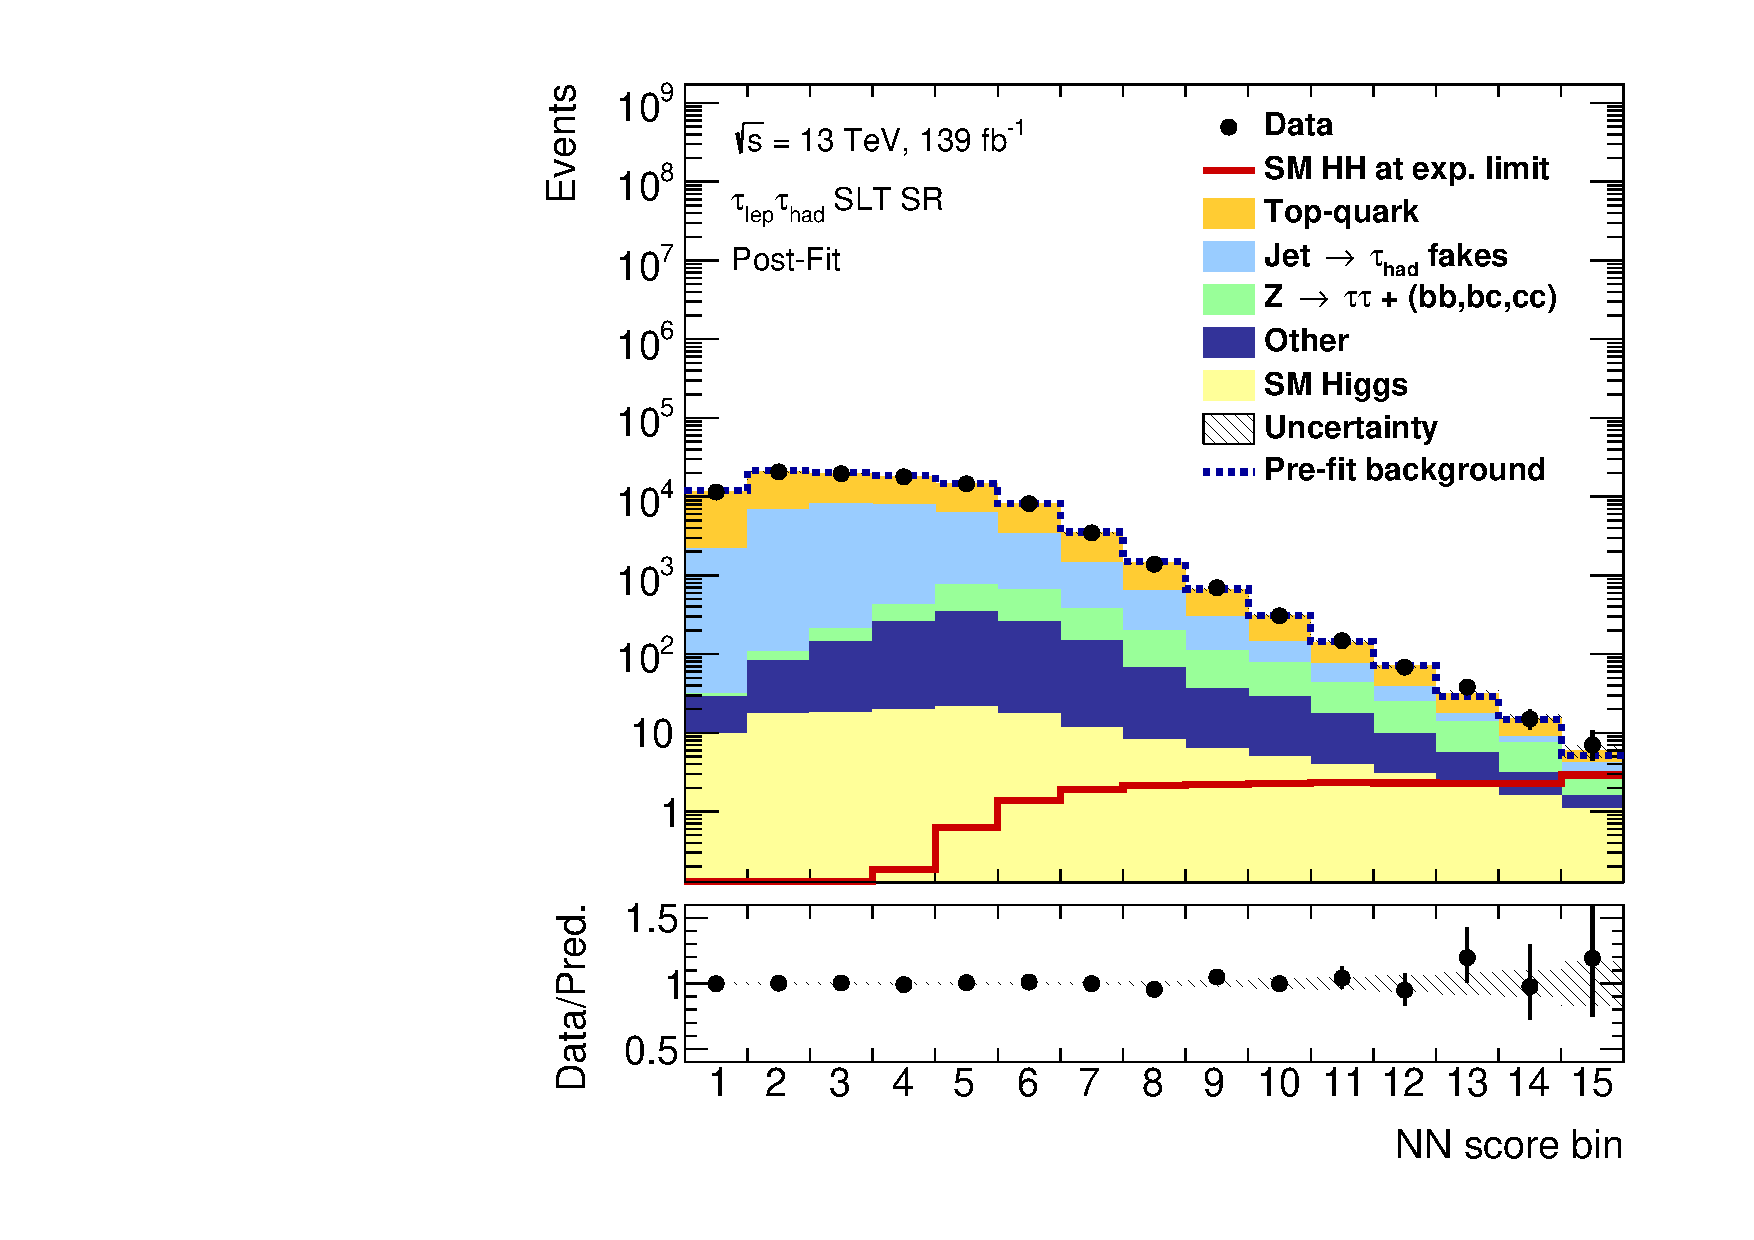
\includegraphics[width=\textwidth]{results_nonres/postfit/Region_BMin0_incJet1_distNN_J2_DSM_T2_SpcTauLH_Y2015_LTT0_L1_GlobalFit_conditionnal_mu0log}

    \subcaption{\lephad SLT channel}
  \end{subfigure}\hfill%
  \begin{subfigure}{0.495\textwidth}
    \centering

    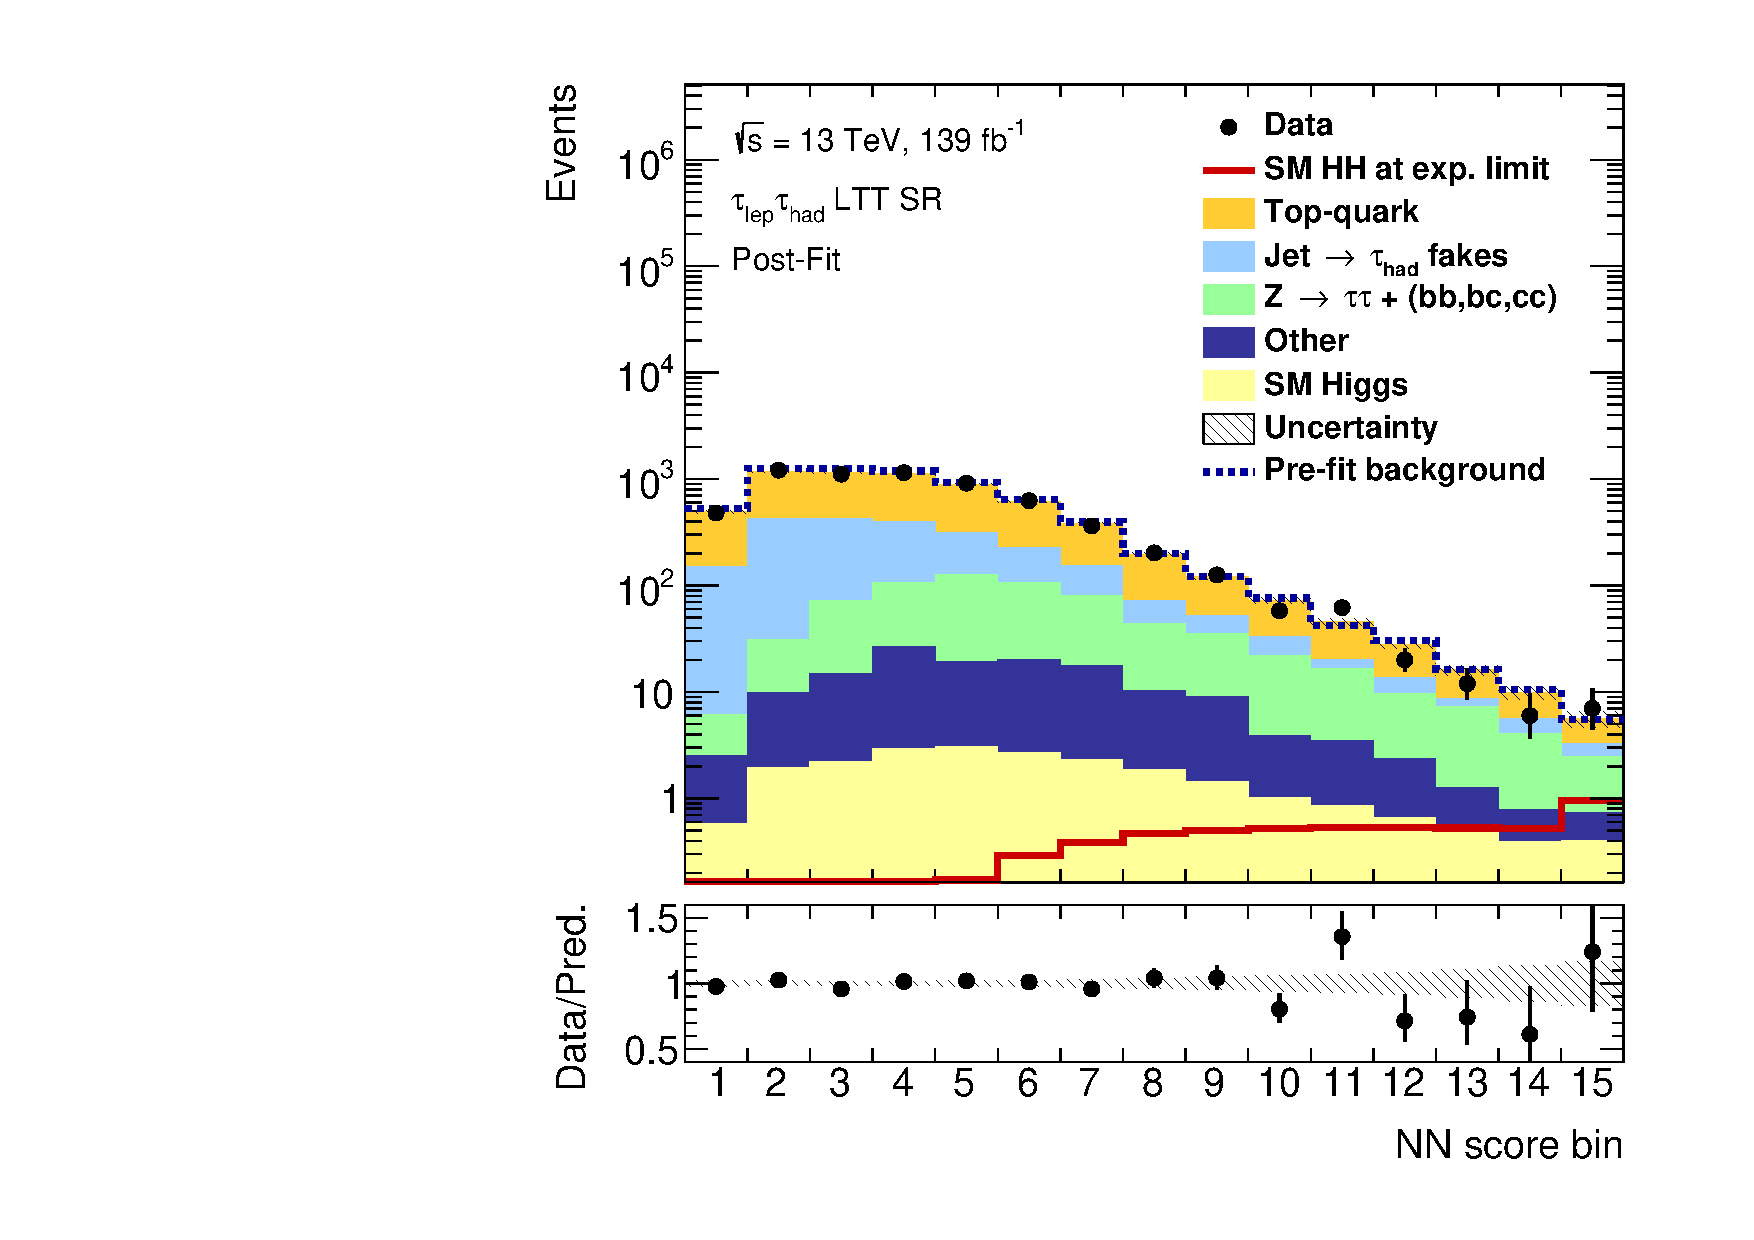
\includegraphics[width=\textwidth]{results_nonres/postfit/Region_BMin0_incJet1_distNN_J2_DSM_T2_SpcTauLH_Y2015_LTT1_L1_GlobalFit_conditionnal_mu0log}

    \subcaption{\lephad LTT channel}
  \end{subfigure}

  \vspace{0.5em}

  \begin{subfigure}{0.495\textwidth}
    \centering

    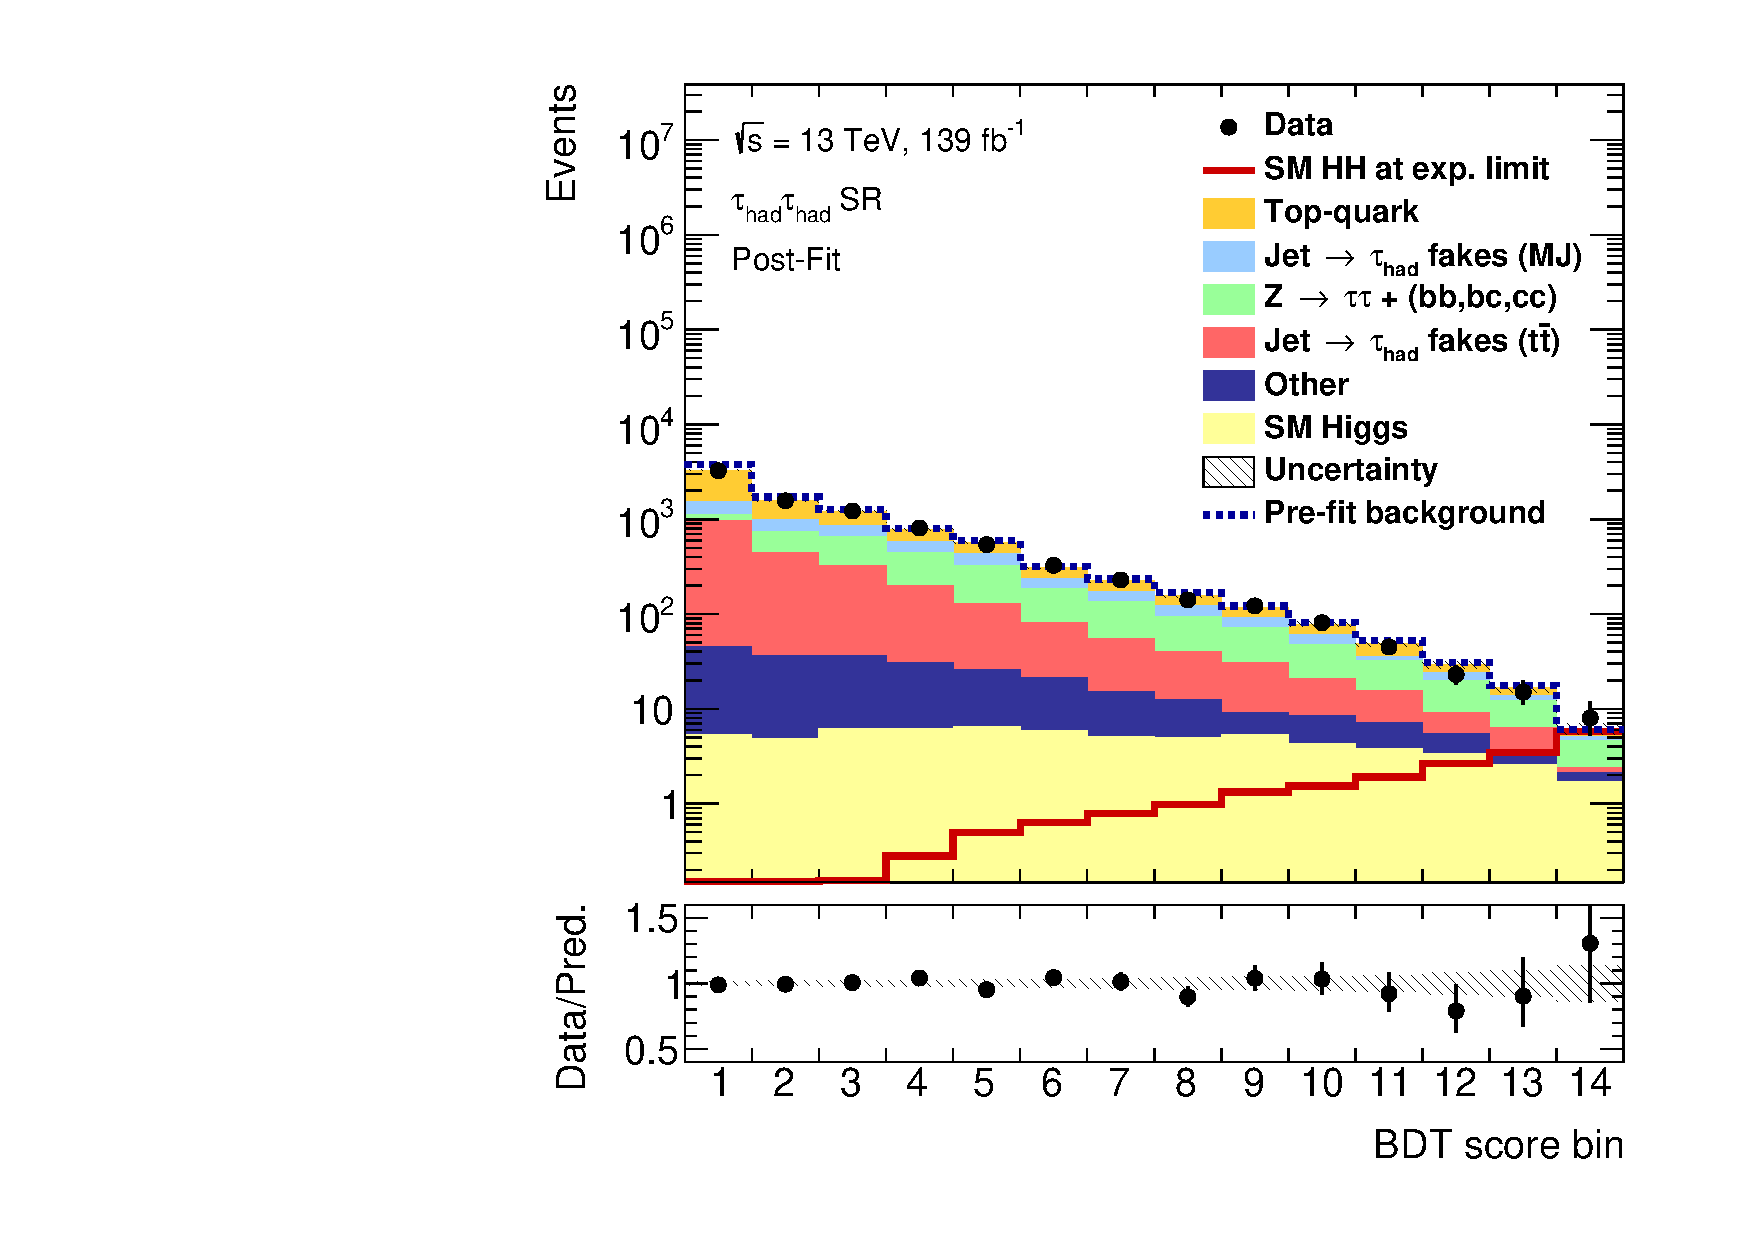
\includegraphics[width=\textwidth]{results_nonres/postfit/Region_BMin0_incJet1_distSMBDT_J2_Y2015_DLLOS_T2_SpcTauHH_L0_GlobalFit_conditionnal_mu0log}

    \subcaption{\hadhad channel}
  \end{subfigure}

  \caption{Distribution of the MVA discriminants used to extract the
    non-resonant SM \HH signal in the \lephad SLT (a), \lephad LTT (b), and
    \hadhad (c) channel after the background-only fit of all signal and control
    regions. The signal overlay is scaled to the expected upper limit on the
    signal strength of $3.9$ from the combination of all channels. The
    \faketauhadvis background in the \hadhad channel is shown separately for
    \faketauhadvis from multi-jet (MJ) and \ttbar.}%
  \label{fig:mvascores_postfit}
\end{figure}

\begin{table}[htbp]
  \centering

  \caption{Expected event yields per physics process in the three signal regions
    (a) and in the two most signal-like bins of the MVA discriminants (b) after
    the background-only fit to the observed data in all regions. The category
    ``other backgrounds'' combines minor contributions from
    $Z \to \tautau + (bl,cl,ll)$, $Z \to e^{+}e^{-}$, $Z \to \mu^{+}\mu^{-}$,
    \Wjets, diboson and $\ttbar V$. The expected SM \HH signal yield is shown
    with $\mu = 1$ and nuisance parameters at their best-fit value except for
    nuisance parameters only affecting the SM \HH signal which are kept at their
    pre-fit values.}

  \begin{subtable}{\textwidth}
    \centering
    \subcaption{Expected event yields in the signal regions}%
    \label{tab:postfit_yields_smhh}

    \begin{tabular}{l
  @{\hskip 20pt}
  S[table-format=4.2(3)]
  @{\hskip 20pt}
  S[table-format=5.1(4)]
  @{\hskip 20pt}
  S[table-format=4.2(3)]}
  \toprule
  & \multicolumn{3}{c}{Signal region event yield} \\
  \cmidrule{2-4}
  Process                              & {\hadhad}    & {\lephad SLT} & {\lephad LTT} \\
  \midrule
  SM \HH (ggF + VBF)                   & 5.16 +- 0.84 & 5.9 +- 1.0    & 1.42 +- 0.24 \\
  \midrule
  Top-quark                            & 3250 +- 160  & 61000 +- 1400 & 4040 +- 200 \\
  $Z \to \tautau + \text{HF}$          & 1550 +- 160  & 1620 +- 130   & 529 +- 57 \\
  Single Higgs boson                   & 66 +- 13     & 148 +- 18     & 23.0 +- 4.3 \\
  Jet $\to \faketauhadvis$ (combined)  & {--}         & 34300 +- 1500 & 1640 +- 170 \\
  Jet $\to \faketauhadvis$ (multi-jet) & 1270 +- 130  & {--}          & {--} \\
  Jet $\to \faketauhadvis$ (\ttbar)    & 2080 +- 200  & {--}          & {--} \\
  Other backgrounds                    & 196 +- 33    & 1308 +- 86    & 121 +- 14 \\
  \midrule
  Total background                     & 8414 +- 90   & 98430 +- 390  & 6357 +- 79 \\
  \midrule
  Observed data                        & 8380         & 98456         & 6351 \\
  \bottomrule
\end{tabular}

%%% Local Variables:
%%% mode: latex
%%% TeX-master: "../phd_thesis"
%%% End:

  \end{subtable}

  \vspace{10pt}

  \begin{subtable}{\textwidth}
    \centering
    \subcaption{Expected event yields in the two most signal-like bins
      of the BDT (\hadhad) and NN (\lephad) discriminants}%
    \label{tab:postfit_yields_smhh_signallike}

    \begin{tabular}{l
  @{\hskip 20pt}
  S[table-format=2.2(3)]
  @{\hskip 20pt}
  S[table-format=2.2(3)]
  @{\hskip 20pt}
  S[table-format=2.3(4)]}
  \toprule
  & \multicolumn{3}{c}{Signal region event yield (signal-like bins)} \\
  \cmidrule{2-4}
  Process                              & {\hadhad}    & {\lephad SLT} & {\lephad LTT} \\
  \midrule
  SM \HH (\ggF + VBF)                   & 2.37 +- 0.39 & 1.34 +- 0.23  & 0.381 +- 0.066 \\
  \midrule
  Top quark                            & 3.80 +- 0.64 & 8.2 +- 1.8    & 6.55 +- 0.89 \\
  $Z \to \tautau + (bb,bc,cc)$         & 8.3 +- 1.2   & 6.0 +- 1.0    & 5.02 +- 0.88 \\
  Single Higgs boson                   & 4.3 +- 1.1   & 2.71 +- 0.51  & 0.79 +- 0.2 \\
  Jet $\to \faketauhadvis$ (combined)  & {--}         & 2.35 +- 0.56  & 2.36 +- 0.84 \\
  Jet $\to \faketauhadvis$ (multi-jet) & 1.94 +- 0.51 & {--}          & {--} \\
  Jet $\to \faketauhadvis$ (\ttbar)    & 2.87 +- 0.46 & {--}          & {--} \\
  Other backgrounds                    & 1.54 +- 0.38 & 1.98 +- 0.24  & 0.72 +- 0.11 \\
  \midrule
  Total background                     & 22.8 +- 1.9  & 21.2 +- 2.1   & 15.4 +- 1.7 \\
  \midrule
  Observed data                        & 23           & 22            & 13 \\
  \bottomrule
\end{tabular}

%%% Local Variables:
%%% mode: latex
%%% TeX-master: "../phd_thesis"
%%% End:

  \end{subtable}

  %%%%%%%%%%%%%%%%%%%%%%%%%%%%%%%%%%%%%%%%%%%%%%%%%%%
  % self.setBkgOthers = {"Zhf", "Zlf", "Zttlf",     %
  %                            "W", "Wtt", "Wjets", %
  %                            "diboson",           %
  %                            "DY", "DYtt",        %
  %                            "ttW", "ttZ"}        %
  %%%%%%%%%%%%%%%%%%%%%%%%%%%%%%%%%%%%%%%%%%%%%%%%%%%

  \todo[inline]{It looks like the error propagation effectively
    symmetrises the error (HH should be asymmetric).}

  \todo[inline]{Have this pre-fit in appendix?}
\end{table}

The choice of analysis strategy of using multivariate discriminants to extract
the signal of interest from loosely preselected events limits the conclusions
that can be drawn regarding the background processes that are relevant to the
signal extraction process. Therefore, \Cref{tab:postfit_yields_smhh_signallike}
lists the expected event yields for the two most signal-like bins of the MVA
discriminants, illustrating the background composition in a phase space
comparable to the one occupied by the signal process.

% Top quark: 3(ttbar):1(stop)
The dominant background in the two most signal-like bins of the SM \HH BDT in
the \hadhad channel is the production of \ZHF with an expectation of about 8
events. The contribution of top quark, single Higgs boson, and \faketauhadvis
backgrounds is similar with an expectation of about 4 events for each
process. The signal efficiency of selecting the two most signal-like bins is
close to \SI{50}{\percent} with respect to the signal yield after pre-selection,
yielding the largest signal-to-background ratio of any individual channel in
this search.

% Top quark (SLT): 1(ttbar):1(stop)
% Top quark (LTT): 5(ttbar):1(stop)
In the \lephad channels the dominant backgrounds in the signal-like bins are
originating from the production of top quarks and \ZHF. Compared to the \hadhad
channel, top quark backgrounds are more abundant\footnote{The targeted
  $\ell + \tauhad$ final state does not distinguish between prompt production of
  electrons / muons and non-prompt production via leptonic \taulepton decays,
  thus both $W \to \taulep \nu_{\tau}$ and $W \to \ell \nu_{\ell}$ ($\ell = e$
  or $\mu$) are considered as \taulepvis candidates. Backgrounds from \ttbar or
  $tW$ production would be about seven times more abundant in the \lephad
  channel compared to the \hadhad channel based on $W$ boson and \taulepton
  branching ratios (taken from Ref.~\cite{pdg2020}) prior to the event
  reconstruction, and disregarding \faketauhadvis contributions.}  with a large
contribution of about \SI{50}{\percent} from single top production in the SLT
channel (ca.\ \SI{15}{\percent} in LTT). The selection of the two most
signal-like bins yields smaller signal efficiencies while having background
rates that are comparable between the three channels. This is due to the
abundance of top quark backgrounds and the larger difficulty of reconstructing
the $H \to \tautau$ candidate in \lephad decay modes, degrading the resolution
of the $\tautau$ and \HH mass reconstruction.

The modelling of MVA input variables in the \hadhad channel can be inspected
in~\Cref{fig:postfit_mva_inputs}, which shows the variables after the
background-only fit of the MVA discriminants to observed data, combining all
channels of the analysis. The post-fit background model describes the observed
data well with minor discrepancies in the angular observables. For example at
low values of \dRtautau the background model tends to overestimate the observed
data by about \SI{10}{\percent} which is not fully covered by uncertainties.

\begin{figure}[htbp]
  \centering

  \begin{subfigure}{0.46\textwidth}
    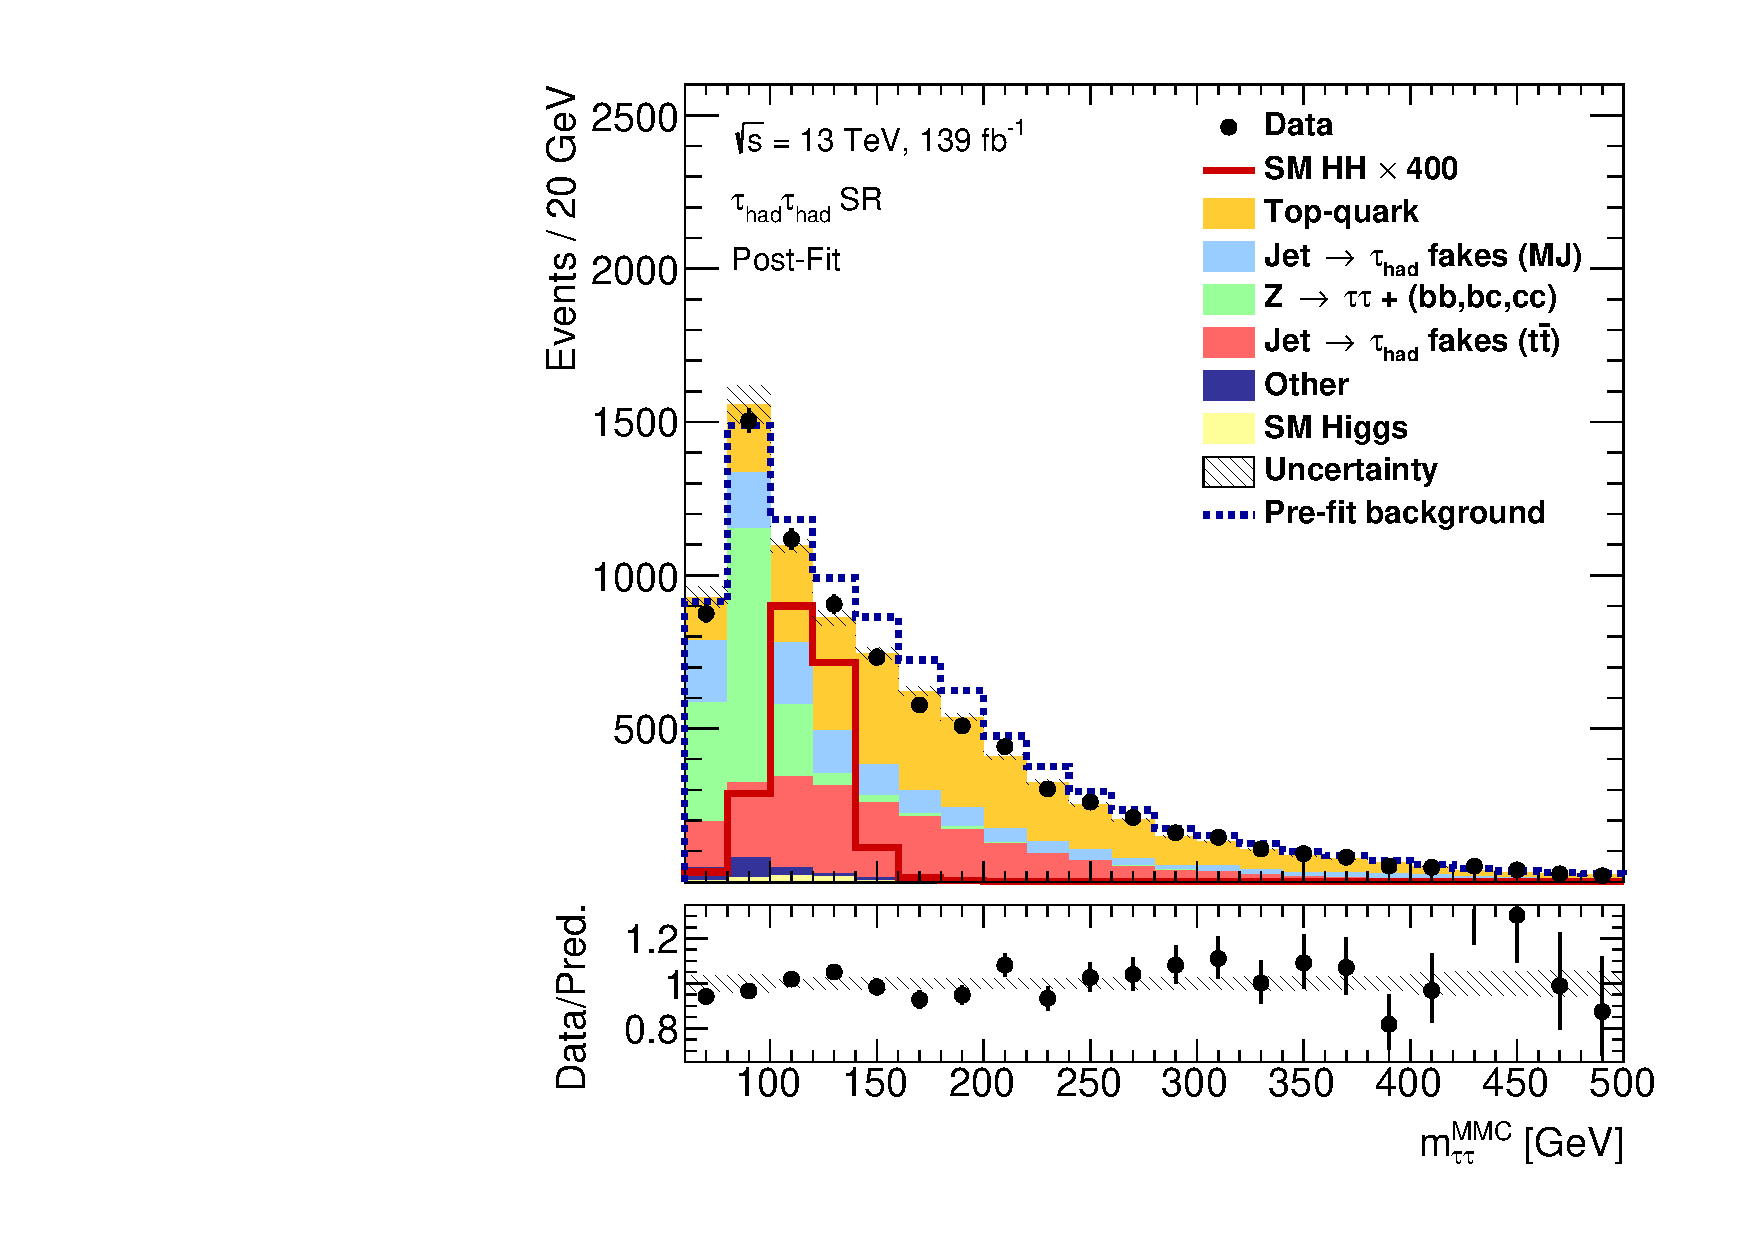
\includegraphics[width=\textwidth]{results_nonres/postfit_mvainputs/Region_BMin0_incJet1_distmMMC_J2_Y2015_DLLOS_T2_SpcTauHH_L0_GlobalFit_conditionnal_mu0}
  \end{subfigure}\hfill%
  \begin{subfigure}{0.46\textwidth}
    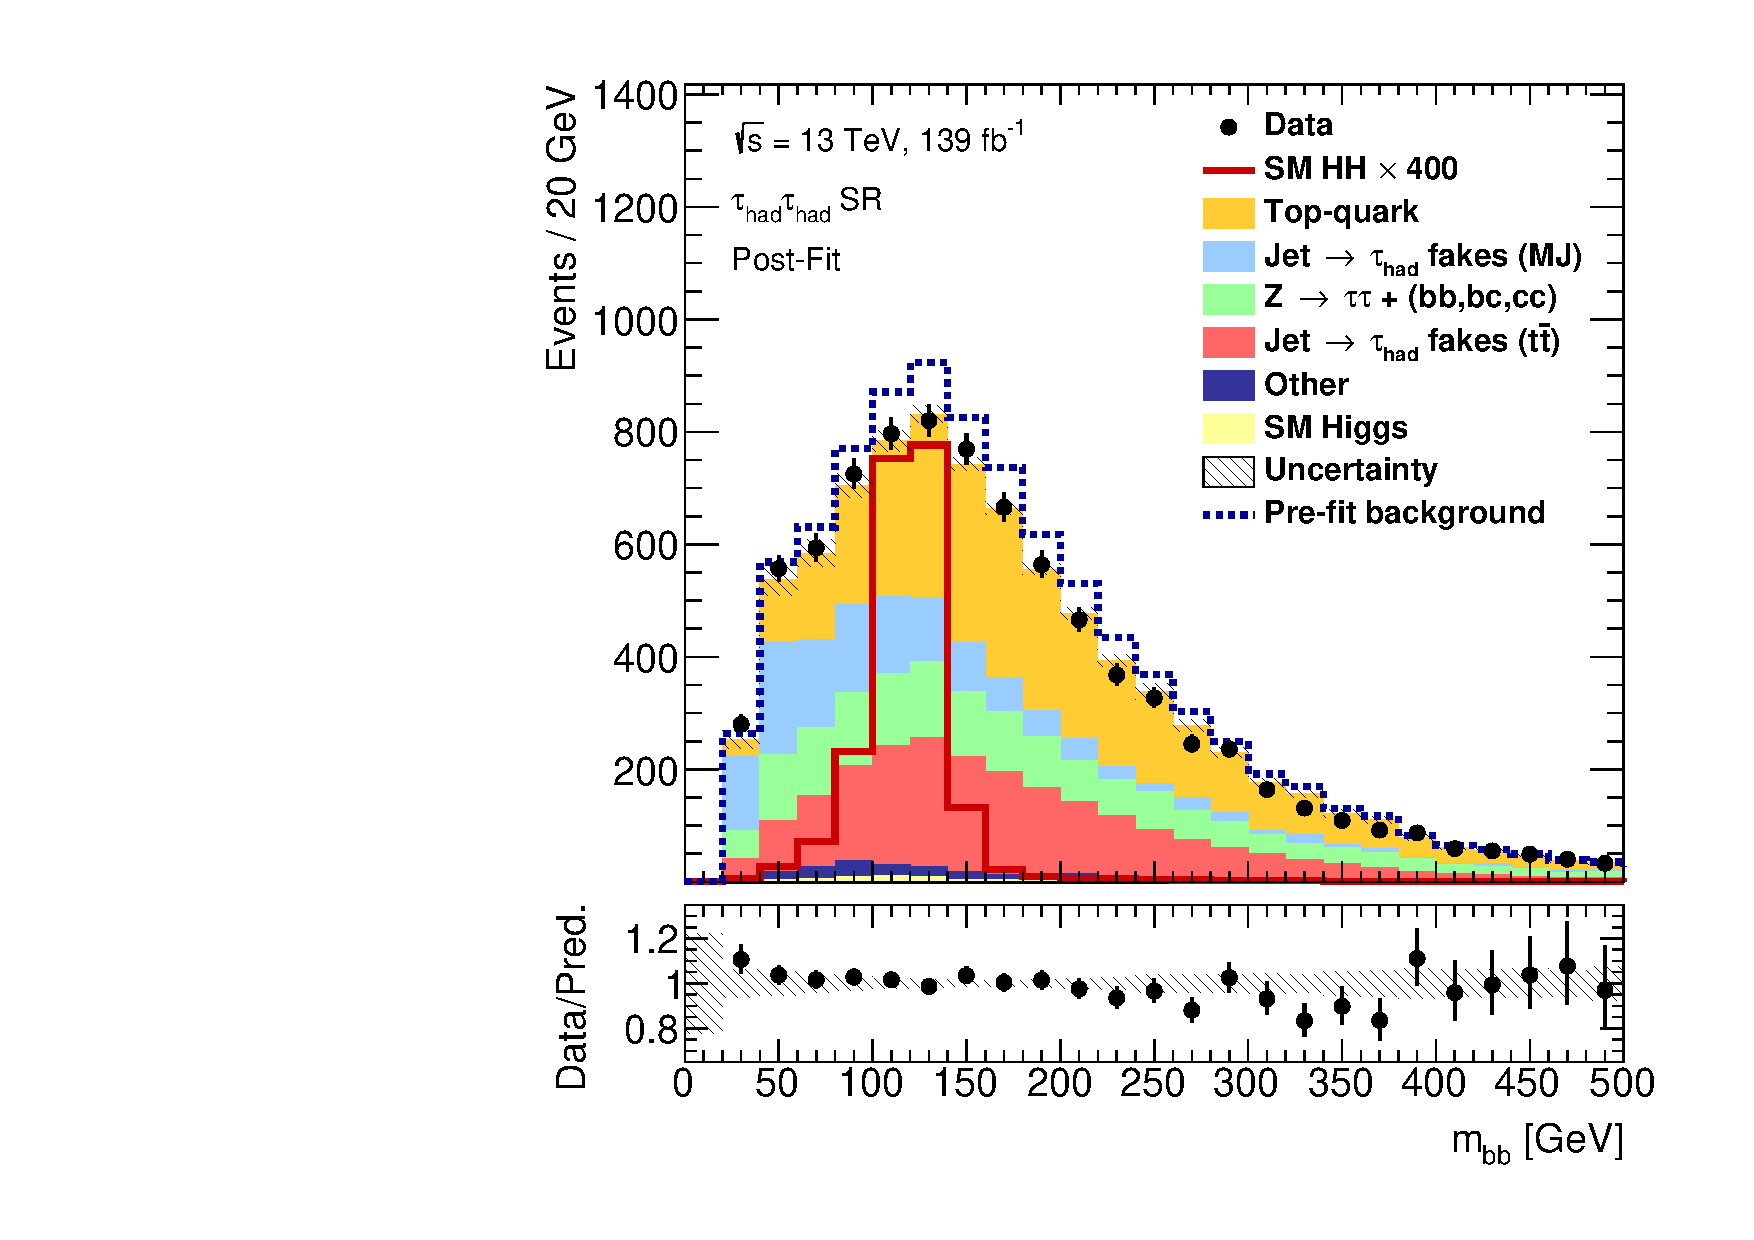
\includegraphics[width=\textwidth]{results_nonres/postfit_mvainputs/Region_BMin0_incJet1_distmBB_J2_Y2015_DLLOS_T2_SpcTauHH_L0_GlobalFit_conditionnal_mu0}
  \end{subfigure}

  \begin{subfigure}{0.46\textwidth}
    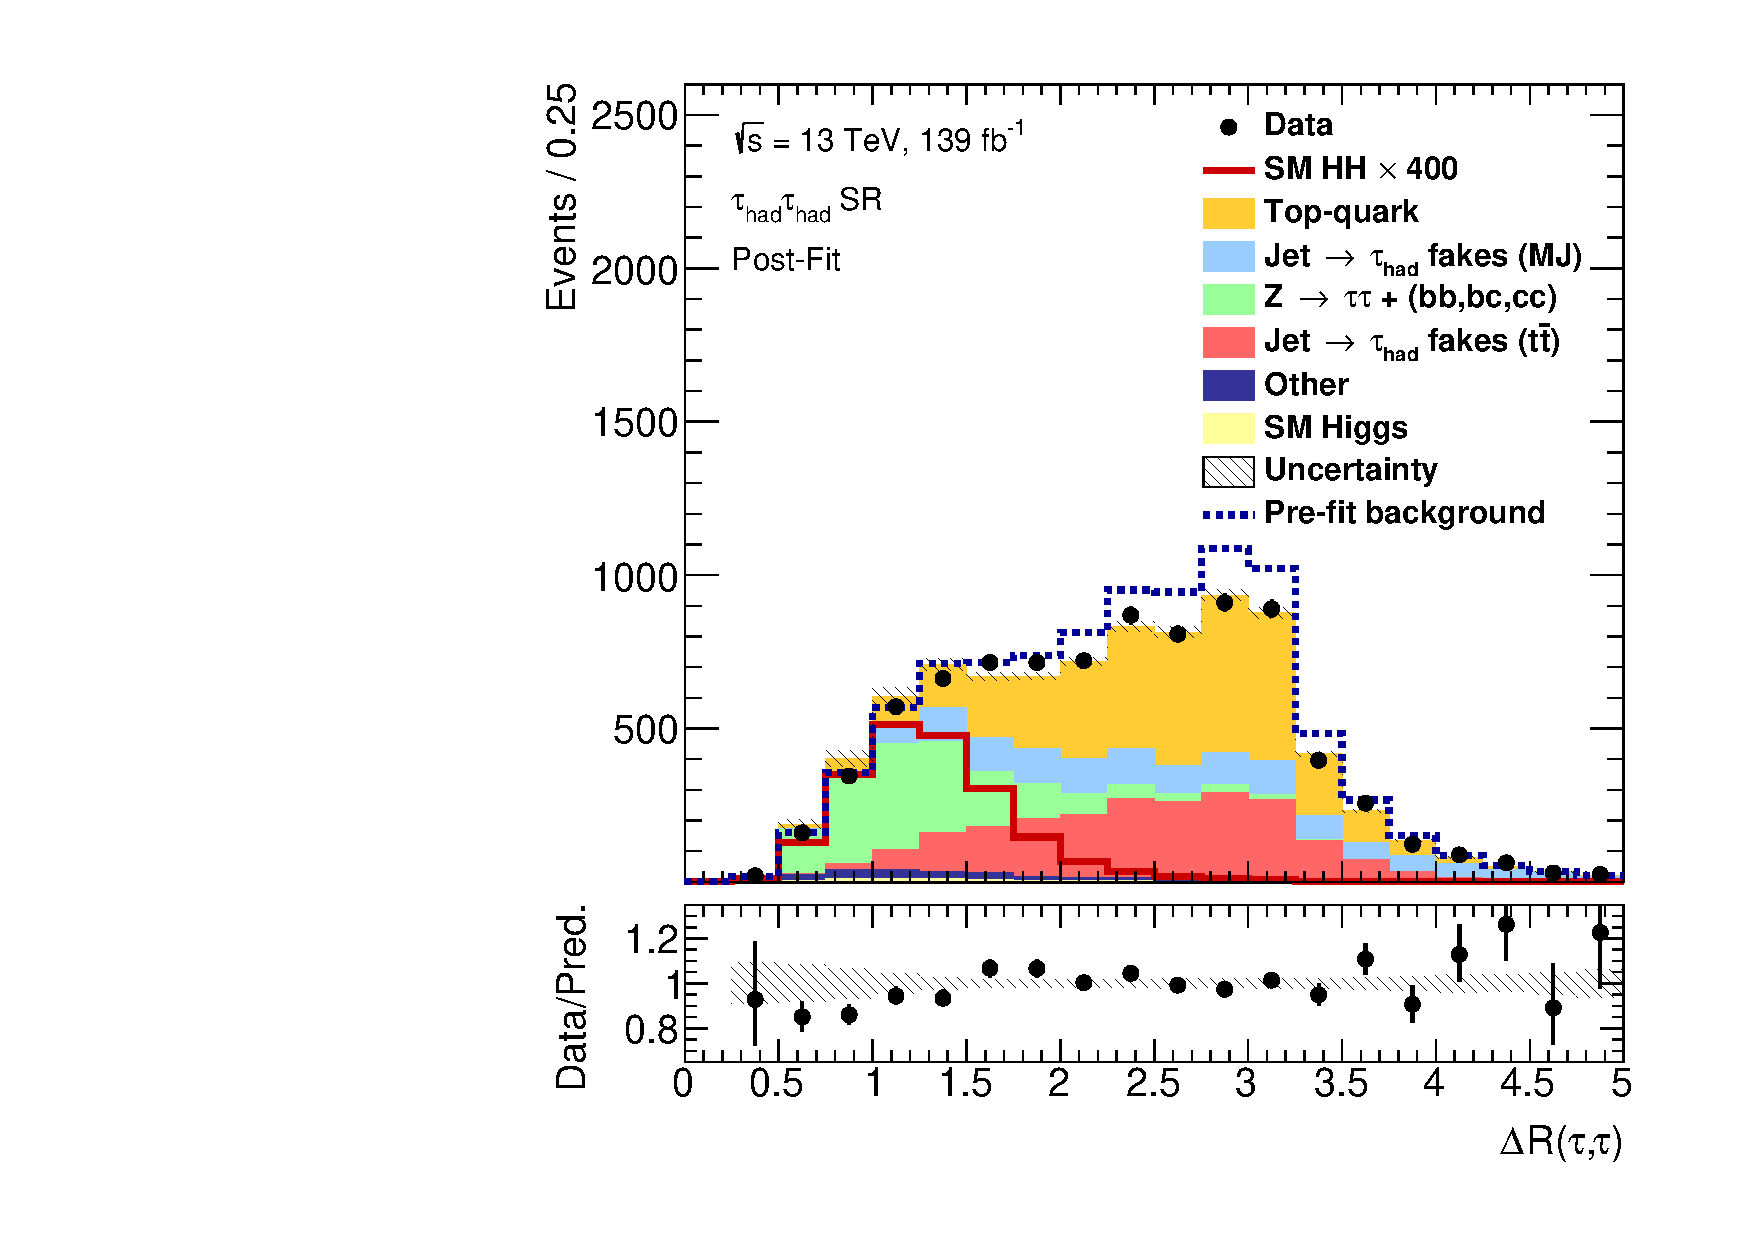
\includegraphics[width=\textwidth]{results_nonres/postfit_mvainputs/Region_BMin0_incJet1_distdRTauTau_J2_Y2015_DLLOS_T2_SpcTauHH_L0_GlobalFit_conditionnal_mu0}
  \end{subfigure}\hfill%
  \begin{subfigure}{0.46\textwidth}
    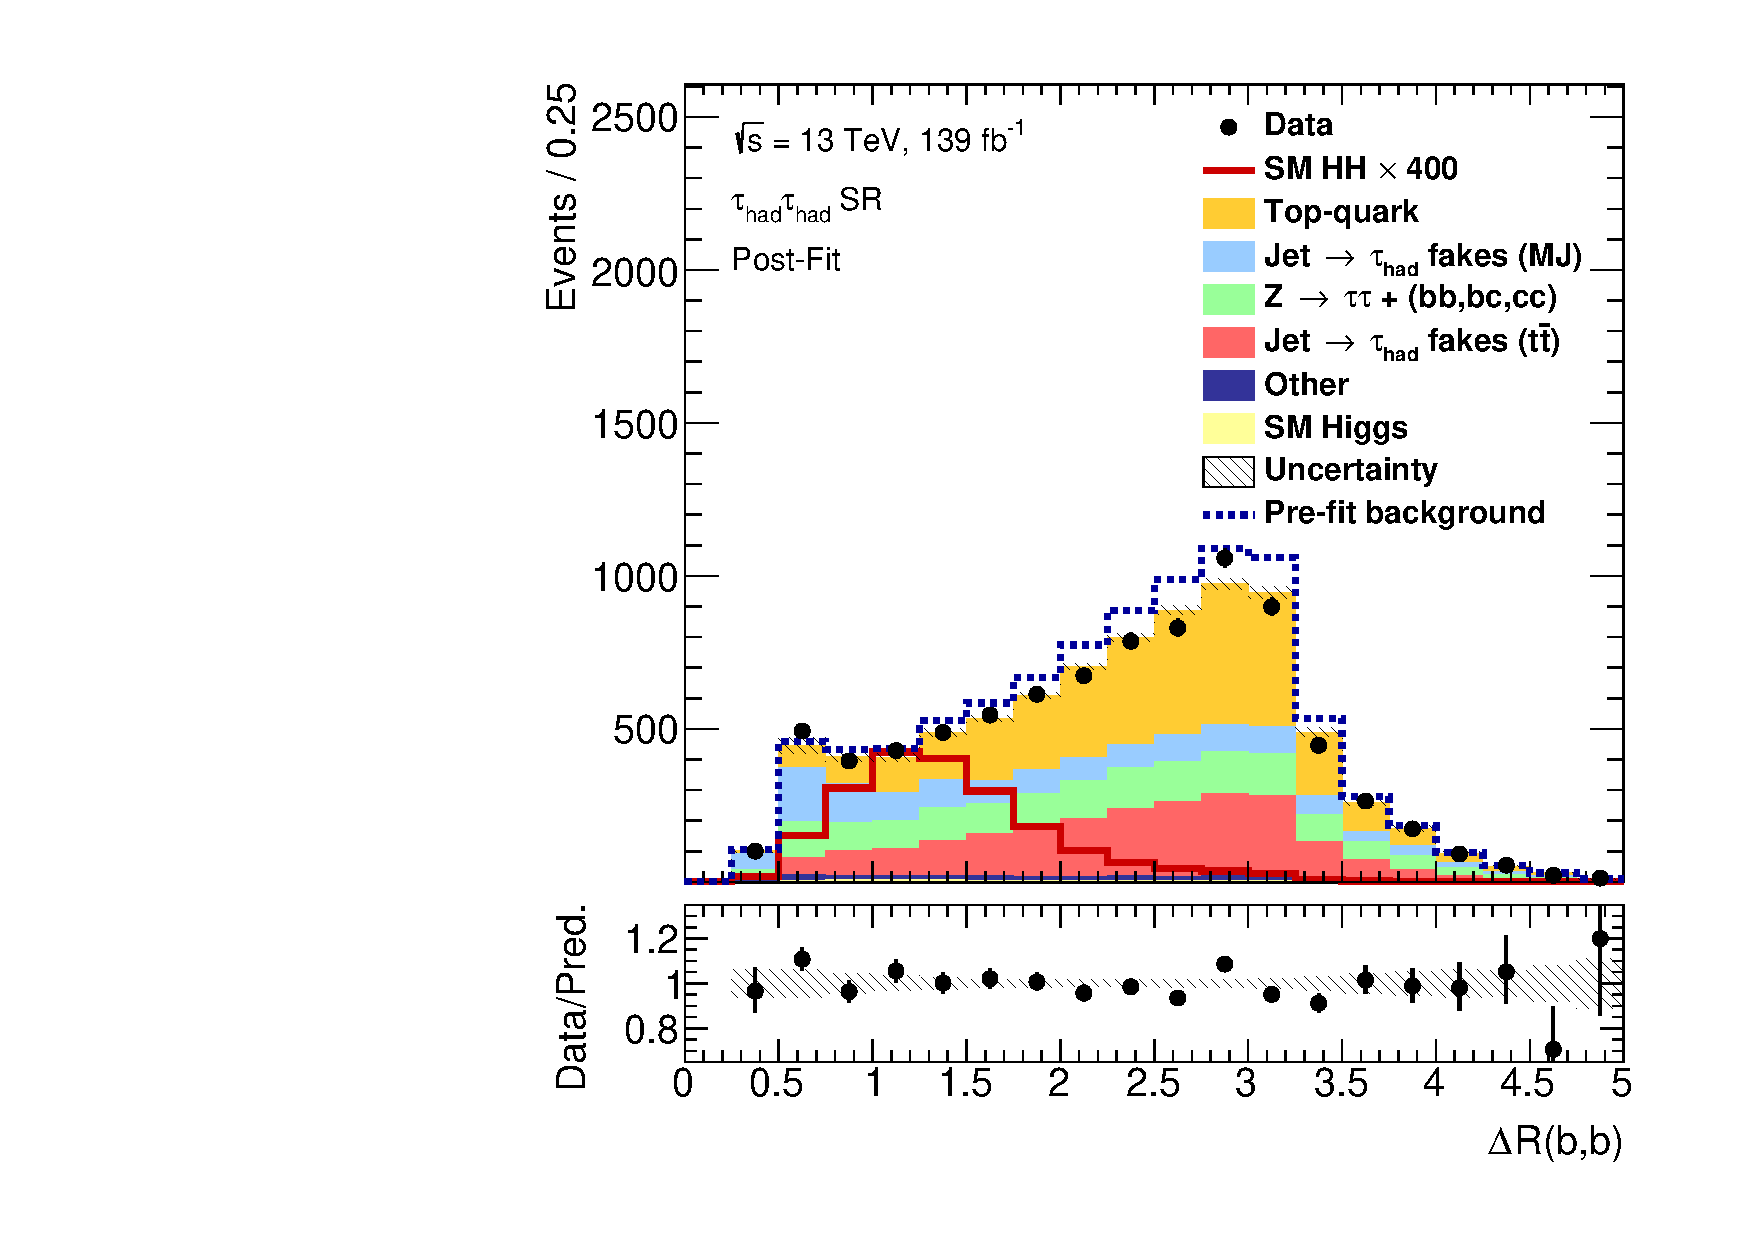
\includegraphics[width=\textwidth]{results_nonres/postfit_mvainputs/Region_BMin0_incJet1_distdRBB_J2_Y2015_DLLOS_T2_SpcTauHH_L0_GlobalFit_conditionnal_mu0}
  \end{subfigure}

  \begin{subfigure}{0.46\textwidth}
    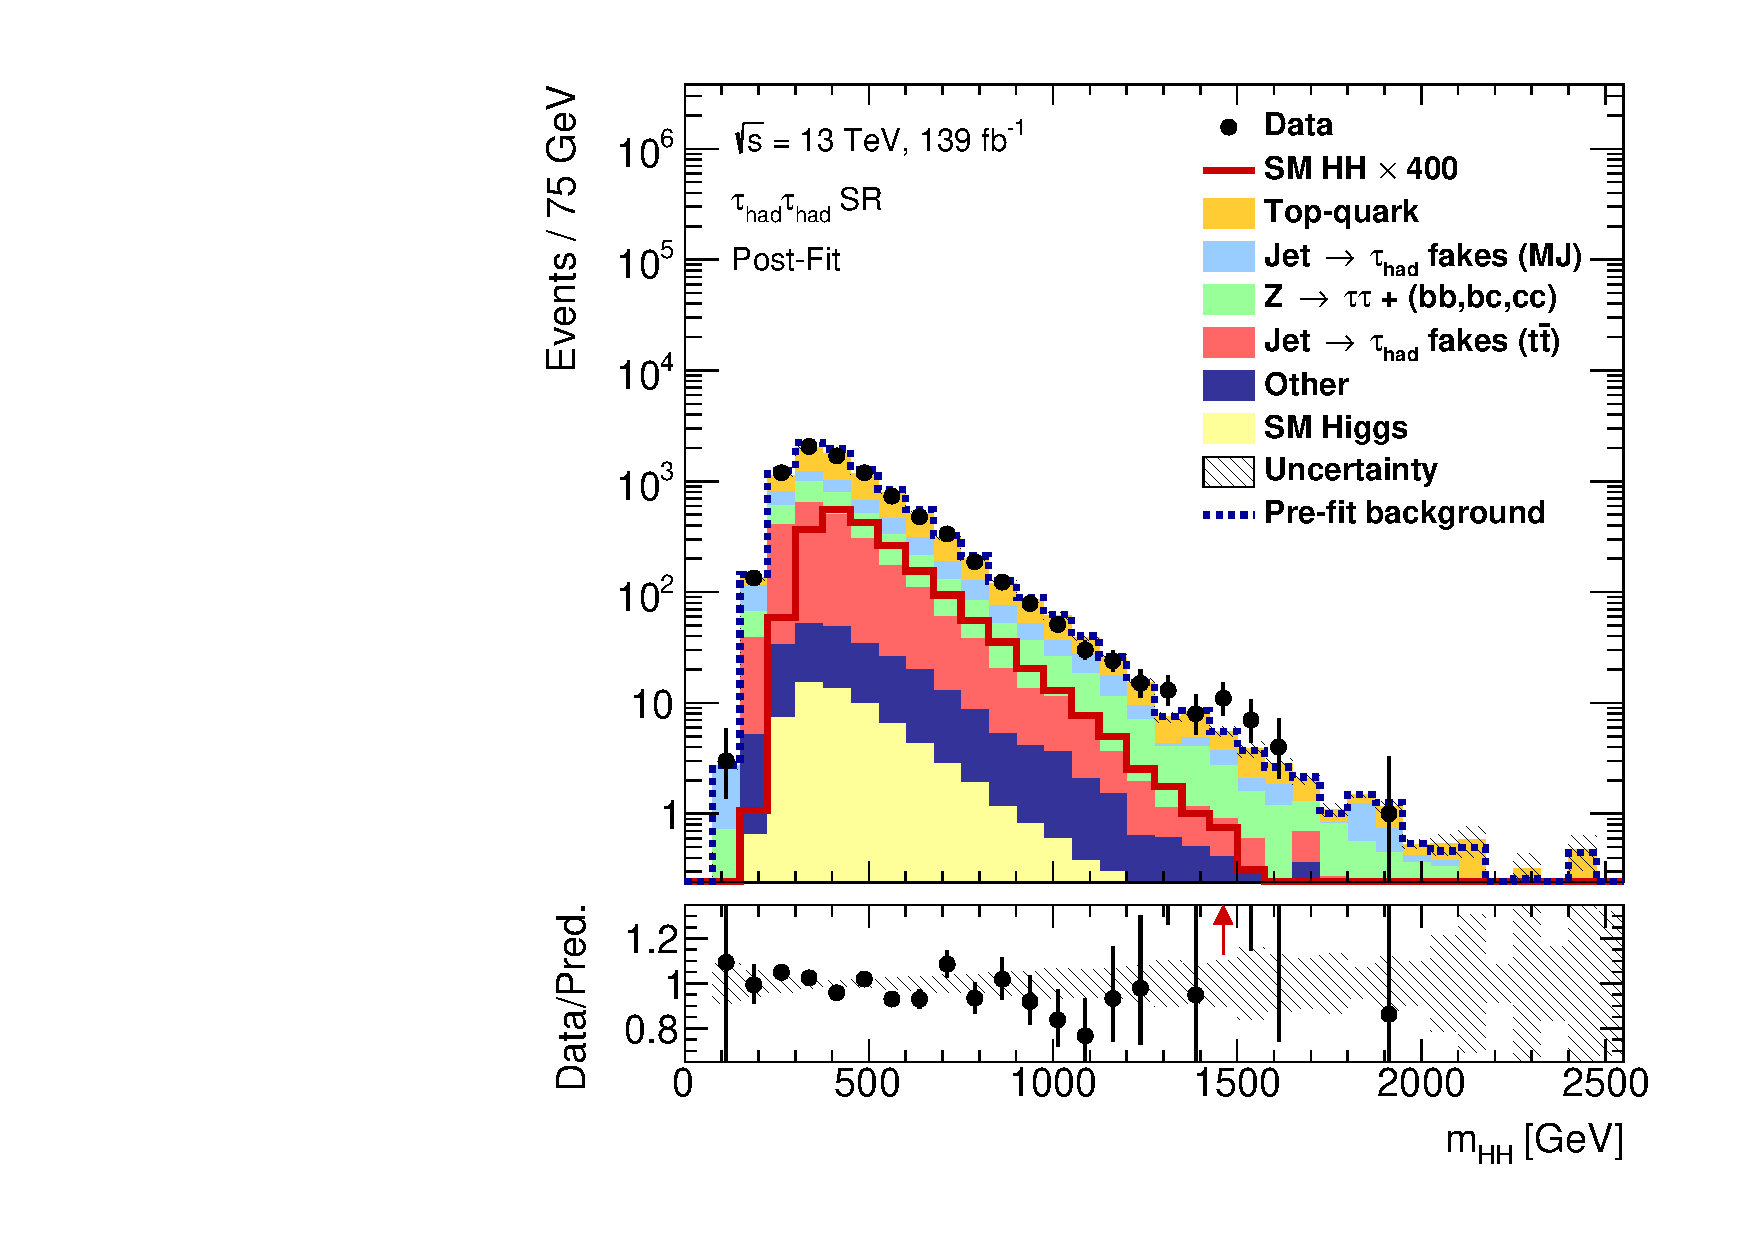
\includegraphics[width=\textwidth]{results_nonres/postfit_mvainputs/Region_BMin0_incJet1_distmHH_J2_Y2015_DLLOS_T2_SpcTauHH_L0_GlobalFit_conditionnal_mu0log}
  \end{subfigure}

  \caption{Distributions of the BDT input variables in the \hadhad signal region
    after the background-only fit of MVA scores and \mll in signal and control
    regions to the observed data. The expected SM $\HH$ signal is overlayed with
    a normalisation corresponding to $\mu = 400$.}
  \label{fig:postfit_mva_inputs}
\end{figure}

A post hoc analysis of the mismodelling observed at low \dRtautau is performed
by examining the dependency of the measured \ZHF normalisation factor as a
function of the transverse momentum of the $Z$ boson by performing a simplified
normalisation measurement in the control region in bins of~$\pT(Z)$
reconstructed from the lepton transverse momenta.\todo{Sentence way too
  long. Rewrite.} This cross-check shows a trend of decreasing \ZHF
normalisation factors with increasing $\pT(Z)$ which can lead to differences of
about \SIrange{5}{10}{\percent} at typical values of $\pT(Z)$ after the \hadhad
pre-selection (approx.\ $\SI{100}{\GeV} < \pT(Z) < \SI{200}{\GeV}$) when
comparing to the $\pT(Z)$-inclusive normalisation factor. Due to the
anticorrelation between $\pT(Z)$ and \dRtautau, this effect can be further
enhanced in regions of low \dRtautau. The acceptance uncertainties on the \ZHF
background, which are derived purely based on simulation, might not fully
account for the effect as it is observed in control region data. In future
analyses it could be beneficial to control for such differential effects when
performing auxiliary measurements of the \ZHF background.\todo{Put a plot in
  appendix?}

% q0 (obs): 0.357911
% sig (obs): 0.598257
% pval (obs): 0.274834

% SM (Asimov mu = 1)
% Median significance: 0.667530
% Median pValue: 0.252217
After visually inspecting the goodness of fit between the background-only model
and the observed data, a formal comparison of the competing hypotheses is
performed. The background-only hypothesis is tested against the alternative that
includes a SM \HH signal with non-negative signal strength using a likelihood
ratio test. The test yields an observed $p_0$-value of \SI{27}{\percent} and
thus the background-only hypothesis cannot be rejected.
% (expected $p_0$-value of \SI{25.2}{\percent} from the $\mu = 1$
% Asimov dataset)
The signal strength obtained from the unconditional fit is
$\hat{\mu} = 0.9\,\numpmerr{+1.8}{-1.5}$ for the combination of all
channels,\footnote{The best-fit signal strength of the fit combining \hadhad
  channel and CR is $\hat{\mu} = 0.7\,\numpmerr{+1.9}{-1.6}$ and for \lephad
  channels and CR, $\hat{\mu} = 1.9\,\numpmerr{+3.7}{-3.2}$.}  which is
compatible with the signal strength in the SM but also with the absence of Higgs
boson pair production.

The dominant uncertainties affecting the measurement of the SM \HH signal
strength are summarised in~\Cref{tab:breakdown_nonres} for the combination of
all channels. The measurement is mainly limited by the statistical uncertainty
originating from the small number of events observed at high values of the MVA
discriminants, explaining about $\frac{2}{3}$ of the variance on
\muhat. Systematic uncertainties play a sub-leading role explaining the
remaining third of the total variance on \muhat. The largest sources of
systematic uncertainty are originating from the modelling of the SM backgrounds
and the statistical precision of the background estimate.

\begin{table}[htbp]
  \centering

  \caption{Decomposition of the variance of $\hat{\mu}$ by uncertainty category
    for the maximum likelihood fit to the observed data in all regions. The
    fraction of the variance on $\hat{\mu}$ from a category is approximated
    using
    $(\Delta\hat{\mu}^2_{\text{tot}} - \Delta\hat{\mu}^2_{\text{w/o cat}}) /
    \Delta \hat{\mu}^2_{\text{tot}}$, where $\Delta\hat{\mu}^2_{\text{tot}}$ is
    the estimate of the total variance of the MLE of $\mu$ and
    $\Delta\hat{\mu}^2_{\text{w/o cat}}$ its variance after fixing the nuisance
    parameters of a category to their best-fit value. The variance of
    $\hat{\mu}$ from data statistical uncertainties is determined directly from
    the model with all nuisance parameters fixed to their best-fit values. The
    fractions of subcategories do not necessarily sum to the fraction of the
    parent category due to correlations between nuisance parameters.}

  % Estimated on non-resonant mu workspace
%
% Fractional impact of nuisance parameter sets, quadratically substracted from total.
% DataStat                     : + 0.649570732823647 / - 0.666811562391472 +- 0.657514352093487
% FullSyst                     : + 0.350429267176353 / - 0.333188437608528 +- 0.34240352840741
% All normalizations           : + 0.00256462411687674 / - 0.000629420848733356 +- 0.00150751388445714
% All but normalizations       : + 0.349881073822931 / - 0.332721677350132 +- 0.341893417327329
% Jets MET                     : + 0.00611881491094716 / - 0.00531445193052364 +- 0.00573985723146677
% BTag                         : + 0.00273018206308313 / - 0.00251352205815197 +- 0.00262889128845151
% Electron Muon                : + 0.00147658980045641 / - 0.000764053590433247 +- 0.0011182187740484
% Tau                          : + 0.00557804691013822 / - 0.00126289813038191 +- 0.0032018485963158
% Pileup reweighting           : + 6.42848069842953e-05 / - 0.000110024034672235 +- 8.39149975446109e-05
% Fake estimation              : + 0.0073527804179163 / - 0.00585172181539581 +- 0.00663745433087985
% Luminosity                   : + 0.00149085233805505 / - 0.000167571652278191 +- 0.000715242667614943
% Top Modelling                : + 0.0604793187664376 / - 0.0562464434201449 +- 0.0585030684775916
% Ztautau+HF Modelling         : + 0.00845814093617601 / - 0.0102153499042302 +- 0.00925002791617588
% Single Higgs Modelling       : + 0.0617151711880666 / - 0.107540079213718 +- 0.0813319338742543
% Signal Modelling             : + 0.0941027334483326 / - 0.00501948112092907 +- 0.0390780989113785
% Other backgrounds            : + 0.000775646139682544 / - 0.00124168478503861 +- 0.000977564478036541
% MC stat                      : + 0.0590496581302566 / - 0.10019920077973 +- 0.0767316565018313
% Instrumental (Chris)         : + 0.0168480040103595 / - 0.0109929390836323 +- 0.0139860056583981
% Signal modelling (Chris)     : + 0.0941027334483326 / - 0.00501948112092907 +- 0.0390780989113785
% Background modelling (Chris) : + 0.162826849351099 / - 0.208956381988409 +- 0.183441723017023

\begin{tabular}{lS[table-format=2.0, table-space-text-pre=\textless]}
  \toprule
         & {Explained fraction} \\
  Source & {of variance on $\hat{\mu}$} \\
  \midrule
  \textbf{Data statistical uncertainty} & 66\,\si{\percent} \\  %81\,\si{\percent} \\
  \textbf{Systematic uncertainties} & 34\,\si{\percent} \\  %58\,\si{\percent} \\
  \hspace{0.8em} Instrumental uncertainties & 1\,\si{\percent} \\  %11\,\si{\percent} \\
  \hspace{0.8em} Signal modelling uncertainties & 4\,\si{\percent} \\
  \hspace{0.8em} Background statistical uncertainties & 8\,\si{\percent} \\  %28\,\si{\percent} \\
  \hspace{0.8em} Background modelling uncertainties & 18\,\si{\percent} \\  %42\,\si{\percent} \\
  \midrule
  \hspace{1.6em} -- \hspace{0.2em} Top-quark (incl.\ free normalisation) & 6\,\si{\percent} \\
  \hspace{1.6em} -- \hspace{0.2em} \ZHF (incl.\ free normalisation) & 1\,\si{\percent} \\
  \hspace{1.6em} -- \hspace{0.2em} SM Higgs boson & 8\,\si{\percent} \\
  \hspace{1.6em} -- \hspace{0.2em} Fake-\tauhadvis & {\textless } 1\,\si{\percent} \\
  \hspace{1.6em} -- \hspace{0.2em} Other & {\textless } 1\,\si{\percent} \\
  \bottomrule
\end{tabular}

% {$( \Delta \mu_{\text{tot}}^2 - \Delta \mu_{\text{categ.}}^2  ) / \Delta \mu_{\text{tot}}^2$} \\

%%% Local Variables:
%%% mode: latex
%%% TeX-master: "../phd_thesis"
%%% End:


  \label{tab:breakdown_nonres}
\end{table}

The effect of uncertainties on \muhat is examined on the level of individual
nuisance parameters in~\Cref{fig:nonres_np_rankings} separately for the
combination of all channels and for fits of the \hadhad and \lephad channels
individually. A ranking of the 15 nuisance parameters with the largest impact on
the signal strength estimation is shown, including the MLE of the nuisance
parameters and their \SI{68}{\percent} confidence intervals from the
unconditional fit to observed data.

\begin{sidewaysfigure}[p]
  \centering

  \begin{subfigure}{0.32\textwidth}
    \centering
    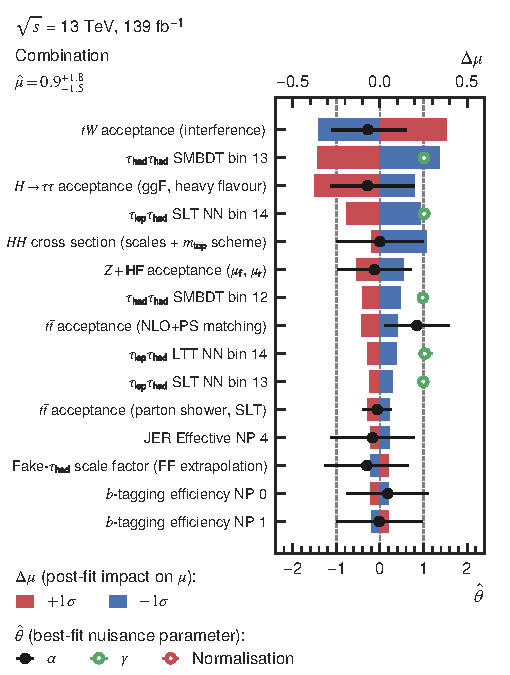
\includegraphics[width=\textwidth]{results_nonres/rankings/ranking_nonres_combined}
    \subcaption{Combination of all channels}
  \end{subfigure}\hfill%
  \begin{subfigure}{0.32\textwidth}
    \centering
    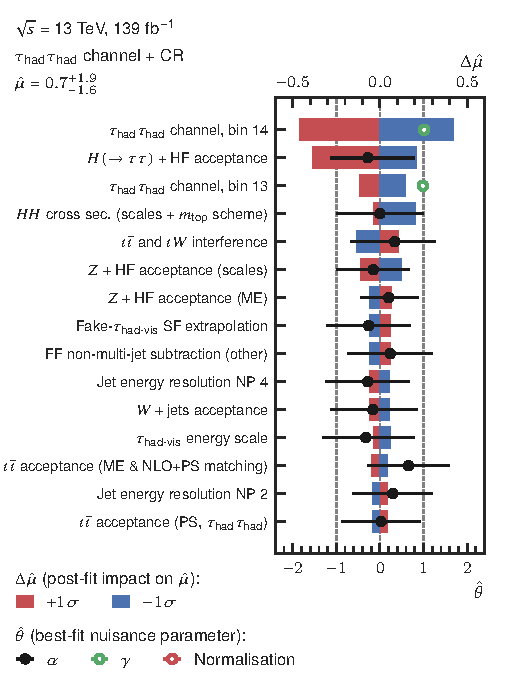
\includegraphics[width=\textwidth]{results_nonres/rankings/ranking_nonres_hadhad}
    \subcaption{\hadhad channel and \ZHF CR}%
    \label{fig:nonres_np_ranking_hadhad}
  \end{subfigure}\hfill%
  \begin{subfigure}{0.32\textwidth}
    \centering
    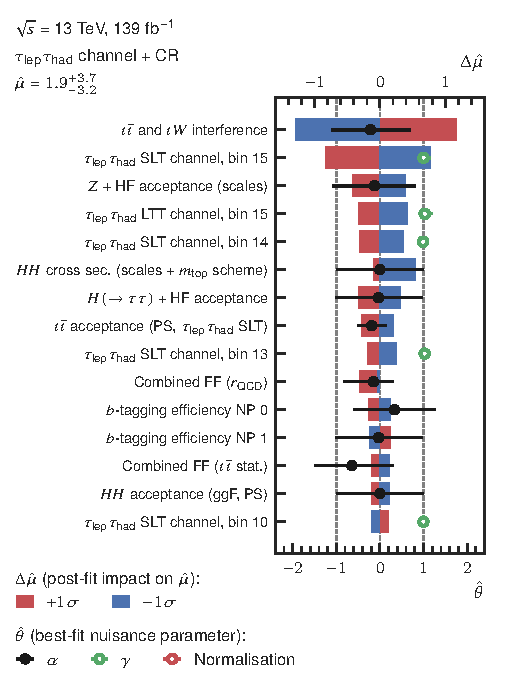
\includegraphics[width=\textwidth]{results_nonres/rankings/ranking_nonres_lephad}
    \subcaption{\lephad channels (SLT \& LTT) and \ZHF CR}
  \end{subfigure}

  \caption{Ranking of the post-fit impact of nuisance parameters on $\mu$ as
    measured by the change in the estimated signal strength ($\Delta \mu$) when
    performing the fit after fixing a nuisance parameter~$\theta$ to
    $\hat{\theta} \pm \Delta \hat{\theta}$, where $\hat{\theta}$ is the MLE and
    $\Delta \hat{\theta}$ the post-fit uncertainty on the nuisance
    parameter. The impact on $\mu$ is shown on the top axis in descending order
    of the mean $|\Delta \mu|$ of the $+\Delta \hat{\theta}$ and
    $-\Delta \hat{\theta}$ variation. The bottom axis shows the MLE of the
    nuisance parameters including their post-fit uncertainty, with marker
    colours indicating the type of nuisance parameter: NP with Gaussian
    constraint ($\alpha$ / black markers), NP with Poisson constraint related to
    the statistical precision of the background estimate ($\gamma$ / green
    markers), and unconstrained normalisation factors (red markers). NP rankings
    and their MLE are obtained from fits of the signal-plus-background model to
    the observed data in all regions (a), in the \hadhad signal region and the
    \ZHF CR (b), in the \lephad signal regions and the \ZHF CR (c).}%
  \label{fig:nonres_np_rankings}
  \todo[inline]{The uncertainties are obtained from the likelihood profile - asymmetric.}
\end{sidewaysfigure}

The 15 highest ranked nuisance parameters show good compatibility with their
values prior to the fit. For few nuisance parameters the fit provides more
stringent constraints than suggested by their prior measurement, which is
consistent with the results obtained from fits to Asimov datasets.

The largest NP constraint observed in the \hadhad channel fit is from the \ZHF
acceptance uncertainty determined from MC-to-MC comparison of \SHERPA and
\MGNLOPY. The uncertainty associated with this NP is expected to be
conservative, since it arises from a comparison of the nominal event generation
at NLO with a prediction lower order of the perturbative expansion (LO).

In the \lephad channel, large constraints are observed on the nuisance parameter
associated to the uncertainty on $r_{\text{QCD}}$ and the \ttbar acceptance
uncertainty from the comparison of parton shower programs. The uncertainty on
$r_{\text{QCD}}$ is derived to be conservative, varying the assumed fraction of
\faketauhadvis originating from multi-jet processes in the anti-\tauhadvis
control region between 0 and \SI{100}{\percent}, explaining the large
constraints on this parameter. The constraints on the \ttbar acceptance
uncertainty based on the parton shower comparison stems from the \lephad SLT
channel which has high purity of top quark backgrounds. Since the constraint is
large, this uncertainty source is de-correlated between channels to avoid
underestimating the acceptance uncertainty in other channels based on the
measurement in the \lephad SLT channel\todo{Should mention this earlier?}.

A few features of the ranking of nuisance parameters / nuisance parameter
categories, as previously presented in \Cref{tab:breakdown_nonres} and
\Cref{fig:nonres_np_rankings}, are highlighted in the following:
\begin{itemize}
\item Statistical uncertainties on the background prediction have a large impact
  when comparing to other systematic uncertainties. These uncertainties arise
  from the finite number of simulated events used for the background predictions
  and the number of control region events used to perform the data-driven
  \faketauhadvis background estimates.

  The distinct features of Higgs boson pair production in the SM allow to
  separate the targeted signal well from most background processes when
  employing multivariate techniques. Therefore, simulation-based background
  predictions, while generally produced with integrated luminosities exceeding
  that of the collected data,\footnote{The data statistical uncertainties, not
    the statistical precision of the background prediction, are the primary
    limitation for the signal extraction as can be seen
    in~\Cref{tab:breakdown_nonres}.} do not populate the region of high MVA
  scores densely, leading to non-negligible statistical uncertainties on the
  background predictions in the most signal-like bins.

  Additionally, the data-driven estimate of the multi-jet background in the
  \hadhad channel includes large subtractions of non-multi-jet events in the
  control region, further degrading the statistical precision of the background
  estimate. As a result, in the \hadhad-only fit the associated nuisance
  parameter has the largest impact of any single NP on the extracted signal
  strength (cf.\ $\gamma$ NP for SMBDT bin 13
  in~\Cref{fig:nonres_np_ranking_hadhad}).

\item The $tW$ acceptance uncertainty derived from comparing simulated events
  with different treatment of the $tW$ and \ttbar interference is the NP with
  the largest impact on \muhat for both the combined and the \lephad-only
  fit. It primarily originates from the \lephad SLT channel where the
  uncertainty on $tW$ can reach up to \SI{80}{\percent} at high NN
  score. Moreover, single top production constitutes about \SI{50}{\percent} of
  the top background at high NN score in the \lephad SLT channel, resulting in a
  large impact of this NP on the signal extraction. This uncertainty has less
  impact in the \hadhad and \lephad LTT channel due to the $tW$ fraction and the
  uncertainty itself being smaller\todo{Technically the LTT uncertainty is about
    the same}.

\item The uncertainty on the acceptance of $gg \to H \to \tautau$ production in
  association with quarks of heavy flavour has a large impact on \muhat. The
  most signal-like bins of the BDT discriminant used in the \hadhad channel
  select a considerable number of single Higgs boson events of which ca.\ X are
  from \ggF leading to large uncertainties (since 100\% is assigned).
\end{itemize}

\todo[inline]{Discussion: Impact of data statistical uncertainties is about the
  same -> Speaks for improvements in CP and the analysis. Instrumental decreased
  in full Run~2. Huge improvements in calibration measurements.} The effect of
uncertainties is similar to the previous Run~2
analysis~\cite{HIGG-2016-16-witherratum} using a partial dataset of $pp$
collisions at $\sqrt{s} = \SI{13}{\TeV}$ with \SI{36.1}{\per\femto\barn}
integrated luminosity.

In the absence of statistical evidence for SM \HH production, upper limits are
set on its signal strength and cross section using the \CLs method at
\SI{95}{\percent} confidence level (cf.\ \Cref{sec:hypotesting}). The exclusion
limits are summarised in~\Cref{tab:limits_non_resonant} separately for the
\lephad and \hadhad channels, and for the combination of all channels.

\begin{table}[htbp]
  \centering

  \caption{Expected and observed upper limits on the the cross section of Higgs
    boson pair production via \ggF and VBF, $\sigma(pp \to HH)$, and the SM \HH
    ($gg$F+VBF) signal strength at \SI{95}{\percent} confidence level using the
    \CLs method. The expected limits are obtained under the assumption of
    $\mu = 0$. Uncertainties on the SM prediction of $\sigma(pp \to \HH)$ are
    not considered when setting limits on the cross section directly.}%
  \label{tab:limits_non_resonant}

  % Workspaces: comb_2022_01_29
  % ==================
% Channel: combined
% Upper limit on mu:
%         Obs.     -2sigma     -1sigma        Exp.     +1sigma     +2sigma
%     4.700596    2.082483    2.795737    3.879976    5.399804    7.238819

% Upper limit on xsec [fb]:
%         Obs.     -2sigma     -1sigma        Exp.     +1sigma     +2sigma
%     136.6652     61.5679     82.6550    114.7102    159.6434    214.0133

% ==================
% ==================
% Channel: hadhad
% Upper limit on mu:
%         Obs.     -2sigma     -1sigma        Exp.     +1sigma     +2sigma
%     4.951880    2.371052    3.183142    4.417624    6.148054    8.241901

% Upper limit on xsec [fb]:
%         Obs.     -2sigma     -1sigma        Exp.     +1sigma     +2sigma
%     145.1928     70.4159     94.5334    131.1952    182.5858    244.7692

% ==================
% ==================
% Channel: lephad
% Upper limit on mu:
%         Obs.     -2sigma     -1sigma        Exp.     +1sigma     +2sigma
%     9.679448    4.205958    5.646506    7.836325   10.905898   14.620128

% Upper limit on xsec [fb]:
%         Obs.     -2sigma     -1sigma        Exp.     +1sigma     +2sigma
%     281.6663    124.3330    166.9173    231.6509    322.3910    432.1879

% ==================
\begin{tabular}{
  lc
  S[table-format=3.1, round-mode=figures, round-precision=2]
  S[table-format=3.1, round-mode=figures, round-precision=2]
  S[table-format=3.1, round-mode=figures, round-precision=2]
  S[table-format=3.1, round-mode=figures, round-precision=2]
  S[table-format=3.1, round-mode=figures, round-precision=2]
  S[table-format=3.1, round-mode=figures, round-precision=2]
  }
  \toprule
  && {Observed} & {$-2\sigma$} & {$-1\sigma$} & {Expected} & {$+1\sigma$} & {$+2\sigma$} \\
  \midrule
  \multirow{2}{*}{\lephad channel} & {$\xsecggfvbf \, / \, \si{\femto\barn}$} & 281.6663 & 124.3330 & 166.9173 & 231.6509 & 322.3910 & 432.1879 \\
                                   & {$\mu$} & 9.679448 & 4.205958 & 5.646506 & 7.836325 & 10.905898 & 14.620128 \\
  \midrule
  \multirow{2}{*}{\hadhad channel} & {$\xsecggfvbf \, / \, \si{\femto\barn}$} & 145.1928 & 70.4159 & 94.5334 & 131.1952 & 182.5858 & 244.7692 \\
                                   & {$\mu$} & 4.951880 & 2.371052 & 3.183142 & 4.417624 & 6.148054 & 8.241901 \\
  \midrule
  \multirow{2}{*}{Combination}     & {$\xsecggfvbf \, / \, \si{\femto\barn}$} & 136.6652 & 61.5679 & 82.6550 & 114.7102 & 159.6434 & 214.0133 \\
                                   & {$\mu$} & 4.700596 & 2.082483 & 2.795737 & 3.879976 & 5.399804 & 7.238819 \\
  \bottomrule
\end{tabular}

%%% Local Variables:
%%% mode: latex
%%% TeX-master: "../phd_thesis"
%%% End:

\end{table}

The observed upper limit on the SM \HH signal strength is \num{4.7} with an
expectation of \num{3.9} for the combination of all channels.  The exclusion is
largely driven by the high sensitivity of the \hadhad channel to the SM \HH
production, providing observed (expected) exclusion limits on $\mu$ of \num{5.0}
(\num{4.4}). Further discussion and interpretation of these results will follow
in~\Cref{sec:result_discussion}.


\subsection{Results of the Search for Resonant Production of $HH$}
\label{sec:results_res}

The search for resonant production of Higgs boson pairs via scalar resonances is
interpreted in terms of the cross section of $pp \to X \to HH$. The
interpretation is analogous to the approach taken for the search for
non-resonant SM \HH production, replacing the BDT / NN discriminants with PNN
discriminants evaluated at the $\mX$ hypothesis of interest. Moreover, the
absence of SM Higgs boson pair production is assumed for this interpretation.

The PNN discriminants in the signal region of the \hadhad channel are shown for
four exemplary mass points in~\Cref{fig:resonant_mva_postfit} after the fit of
the background-only model to the observed data in all analysis channels.
Additionally, \Cref{tab:yields_postfit_resonant} depicts the expected number of
events after the fit in a signal-like region of the PNN discriminant. Figures of
the PNN discriminants for the \lephad SLT and LTT channels are documented
in~\Cref{sec:app_additional_figures}.

\begin{figure}[htbp]
  \centering

  \begin{subfigure}{0.495\textwidth}
    \centering

    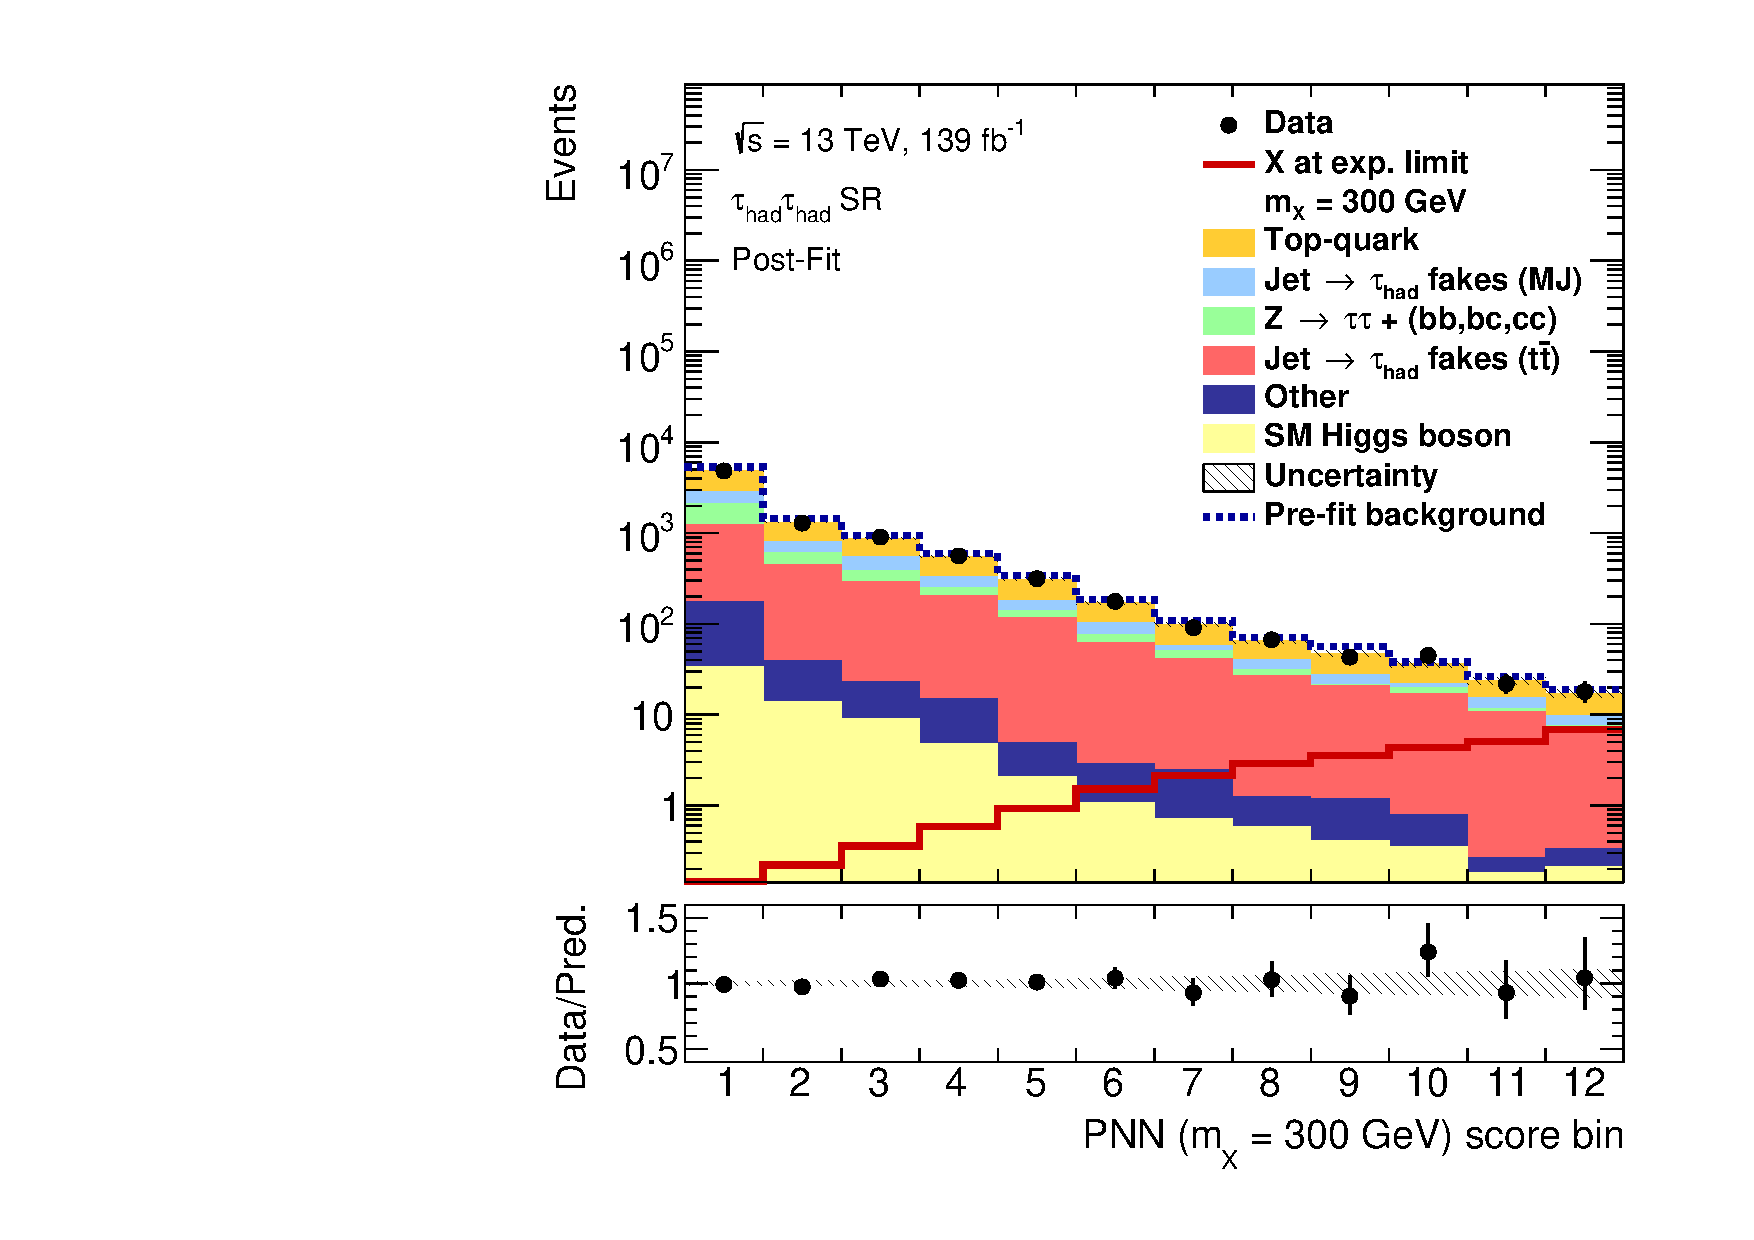
\includegraphics[width=\textwidth]{results_res/postfit/Region_BMin0_incJet1_distPNN300_J2_Y2015_DLLOS_T2_SpcTauHH_L0_GlobalFit_conditionnal_mu0log}
    \subcaption{$\mX = \SI{300}{\GeV}$}
  \end{subfigure}\hfill%
  \begin{subfigure}{0.495\textwidth}
    \centering

    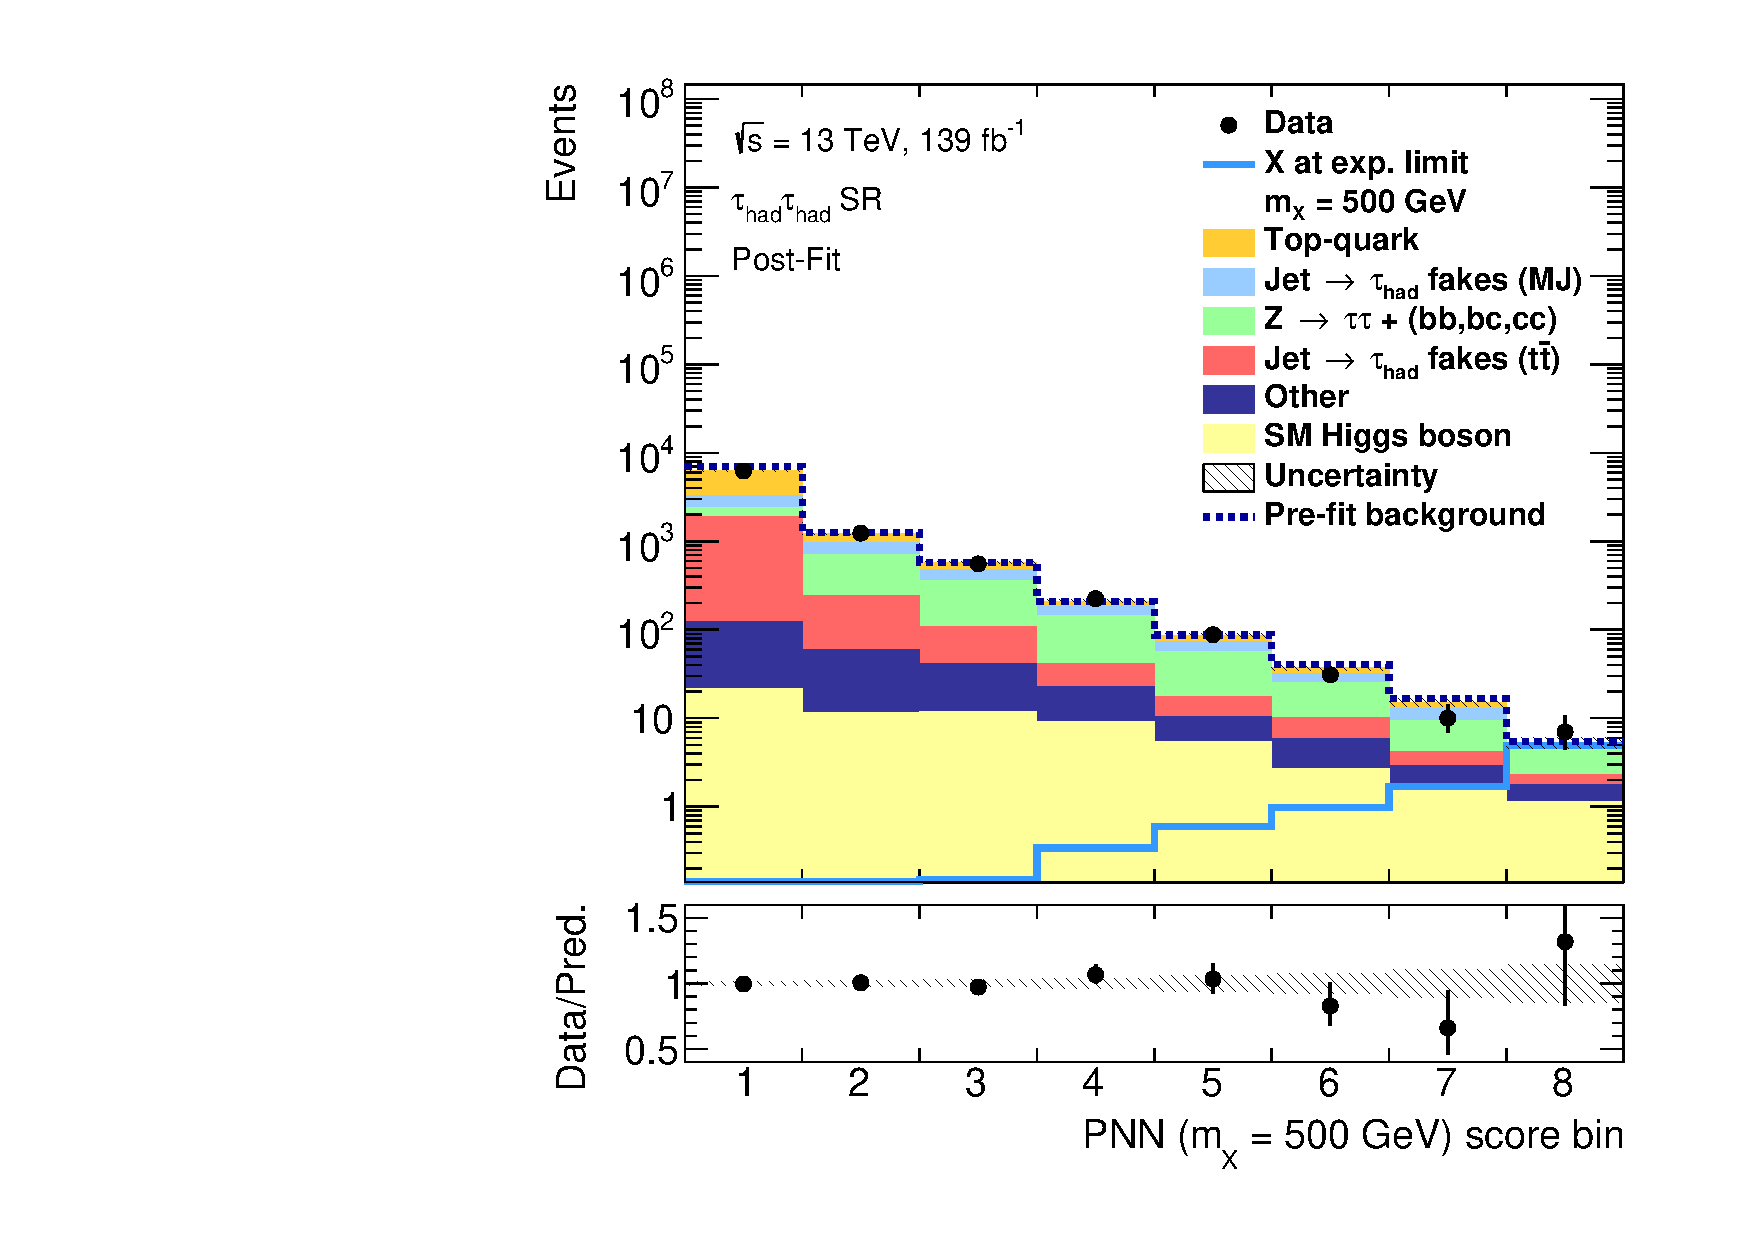
\includegraphics[width=\textwidth]{results_res/postfit/Region_BMin0_incJet1_distPNN500_J2_Y2015_DLLOS_T2_SpcTauHH_L0_GlobalFit_conditionnal_mu0log}
    \subcaption{$\mX = \SI{500}{\GeV}$}
  \end{subfigure}

  \begin{subfigure}{0.495\textwidth}
    \centering

    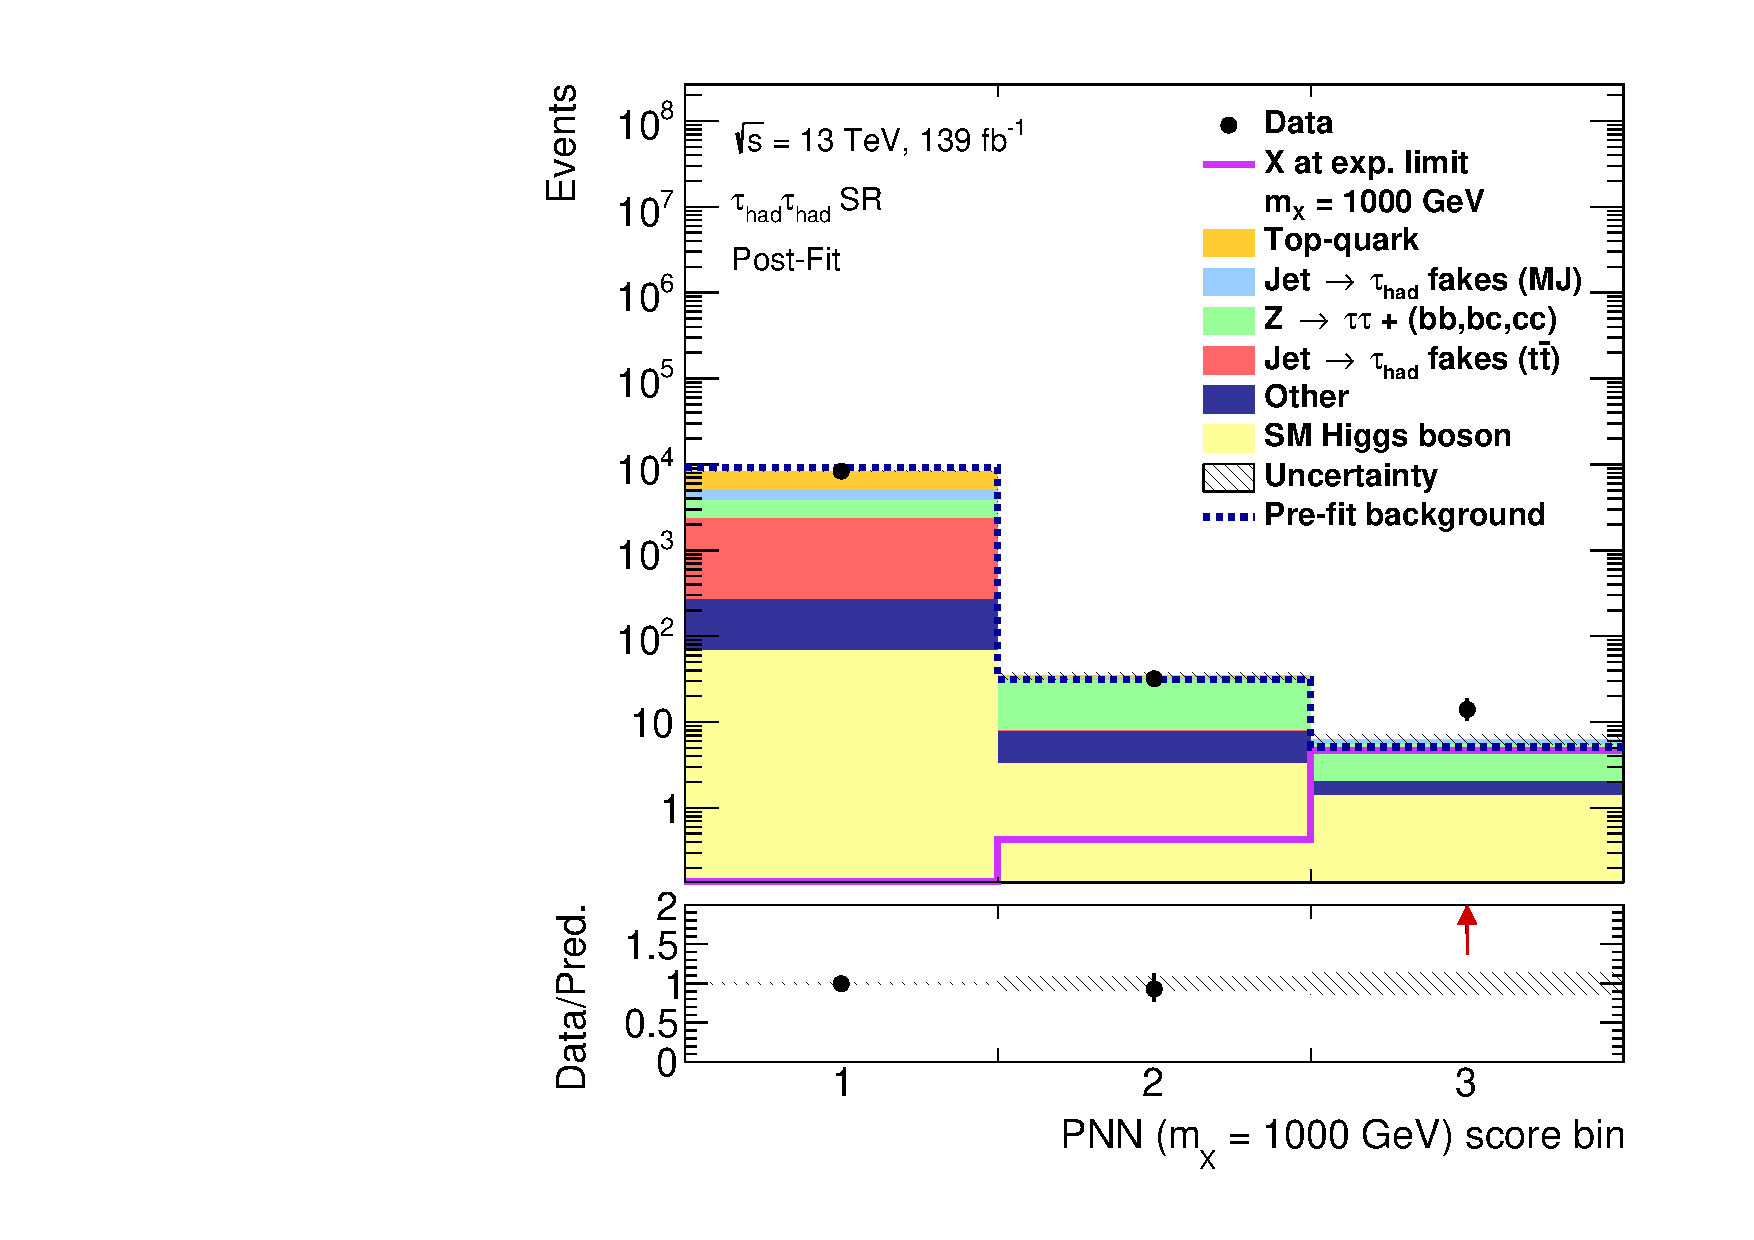
\includegraphics[width=\textwidth]{results_res/postfit/Region_BMin0_incJet1_distPNN1000_J2_Y2015_DLLOS_T2_SpcTauHH_L0_GlobalFit_conditionnal_mu0log}
    \subcaption{$\mX = \SI{1000}{\GeV}$}%
    \label{fig:pnn1000_postfit}
  \end{subfigure}\hfill%
  \begin{subfigure}{0.495\textwidth}
    \centering

    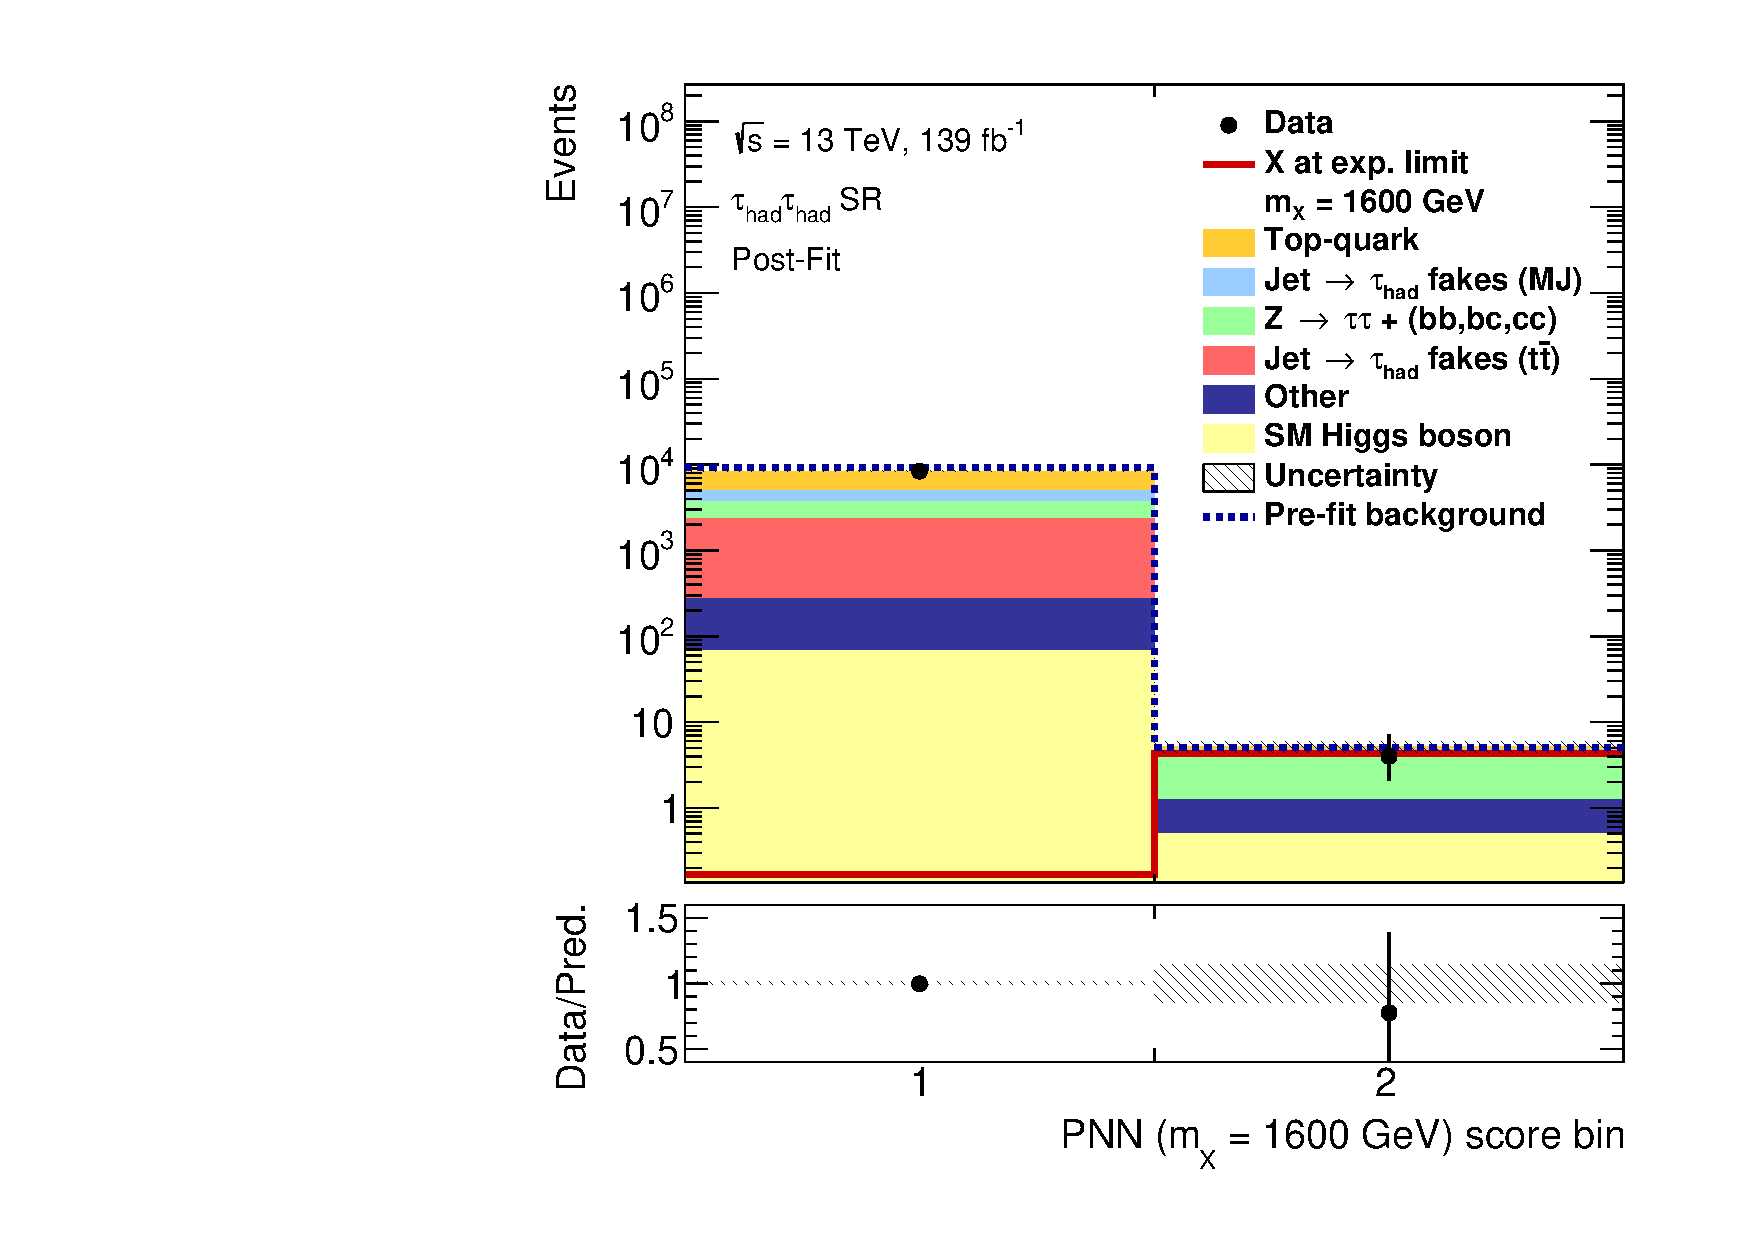
\includegraphics[width=\textwidth]{results_res/postfit/Region_BMin0_incJet1_distPNN1600_J2_Y2015_DLLOS_T2_SpcTauHH_L0_GlobalFit_conditionnal_mu0log}
    \subcaption{$\mX = \SI{1600}{\GeV}$}
  \end{subfigure}

  \caption{Distribution of the PNN discriminant in the \hadhad channel after the
    maximum likelihood fit of the background-only model in all signal and
    control regions. The distributions are shown for four different parameter
    values of the parameterised neural network ranging from \SI{300}{\GeV} to
    \SI{1600}{\GeV}. The signal overlay is scaled to the expected upper limit
    on~$\sigma(pp \to X \to HH)$ for the resonance mass considered.}%
  \label{fig:resonant_mva_postfit}
\end{figure}


\begin{table}[htbp]
  \centering

  \caption{Expected number of events per physics process in the \hadhad signal
    region for signal-like bins of the PNN discriminant after the
    background-only fit to observed data in all regions. The two most
    signal-like bins are shown for $\mX = \SI{300}{\GeV}$ and
    \SI{500}{\GeV}. $\dagger$: The large discrimination power of the PNN for
    large \mX leads to a small number of bins for the statistical interpretation
    due to the choice of re-binning algorithm. Therefore, the expected number of
    events is shown only for the most signal-like bin for
    $\mX = \SI{1000}{\GeV}$ and \SI{1600}{\GeV}.}%
  \label{tab:yields_postfit_resonant}

  \resizebox{\textwidth}{!}{%
    \begin{tabular}{lc
  %@{\hskip 12pt}
  S[table-format=3.2(2)]
  @{\hskip 12pt}
  S[table-format=3.2(2)]
  @{\hskip 12pt}
  S[table-format=3.2(2)]
  @{\hskip 12pt}
  S[table-format=3.2(2)]
  }
  \toprule
  && \multicolumn{4}{c}{Event yield in the most signal-like bin(s)} \\
  \cmidrule{2-6}
  Process                              & $\mX$ & {\SI{300}{\GeV}} & {\SI{500}{\GeV}} & {\SI{1000}{\GeV} ($\dagger$)} & {\SI{1600}{\GeV}  ($\dagger$)} \\
  \midrule
  $X \to HH$ ($\sigma = \SI{1}{\pico\barn}$)
                                       && 18.2 +- 2.9    & 156 +- 16    & 379 +- 38      & 139 +- 28      \\
  \midrule
  Top quark                            && 15.6 +- 2.0    & 2.70 +- 0.44 & 0.12 +- 0.03   & 0.37 +- 0.05   \\
  $Z \to \tautau + (bb,bc,cc)$         && 1.38 +- 0.26   & 7.7 +- 1.1   & 3.50 +- 0.65   & 3.12 +- 0.54   \\
  Single Higgs boson                   && 0.40 +- 0.07   & 2.91 +- 0.61 & 1.40 +- 0.42   & 0.5 +- 0.27    \\
  Jet $\to \faketauhadvis$ (multi-jet) && 5.89 +- 0.92   & 3.48 +- 0.64 & 0.63 +- 0.12   & 0.42 +- 0.07   \\
  Jet $\to \faketauhadvis$ (\ttbar)    && 17.4 +- 2.3    & 1.89 +- 0.28 & 0              & 0              \\
  Other backgrounds                    && 0.21 +- 0.03   & 1.75 +- 0.34 & 0.65 +- 0.13   & 0.74 +- 0.15   \\
  \midrule
  Total background                     && 40.9 +- 3.1    & 20.4 +- 1.9  & 6.29 +- 0.88   & 5.15 +- 0.74   \\
  \midrule
  Observed data                        && 40             & 17           & 14             & 4              \\
  \bottomrule
\end{tabular}

%%% Local Variables:
%%% mode: latex
%%% TeX-master: "../phd_thesis"
%%% End:

  }
\end{table}

The backgrounds relevant to the signal extraction change when considering signal
hypothesis of different \mX. For the search of scalar resonances at low mass,
the dominant background are top quark production and backgrounds with jets being
misidentified as \tauhadvis. These background processes become less relevant as
larger \mX are considered, with the production of \Zjets becoming the dominant
contribution at intermediate masses.

The comparison of the PNN distributions after the background-only fit with the
observed data show decent agreement with exception of the PNN discriminant for
resonances with $\mX = \SI{1000}{\GeV}$ shown in~\Cref{fig:pnn1000_postfit}. In
the most signal-like bin of the corresponding PNN distribution 14 events are
observed, while the background-only model predicts a total of \num{6.29 +- 0.88}
events. This represents a large excess in the number of observed events over the
expectation.

% Pvalues
% Comb: 0.0012948798248544335
% Hadhad: 0.00233581755310297
% Lephad: 0.1208430826663971
%
% Significances
% Comb: 3.0126516970870054
% Hadhad: 2.828844777446568
% Lephad: 1.1707826205098675
The background-only and the signal-plus-background models are compared using a
likelihood ratio test separately for all considered signal hypotheses. The
combination of all analysis channels yields an excess at $\mX = \SI{1000}{\GeV}$
with an observed $p$-value of $\num{1.3e-3}$ and is therefore significant at a
level of $\num{3.0}\,\sigma$.\footnote{By convention in HEP the discovery
  significance is expressed in terms of $\sigma$ given by $\Phi^{-1}(1 - p)$,
  where $\Phi^{-1}$ is the inverse cumulative distribution function (quantile
  function) of the Standard Normal distribution and $p$ the $p$-value of the
  test.} The excess is localised in the \hadhad channel with a significance of
$\num{2.8}\,\sigma$ when performing the test by only including the \hadhad
signal region and the \ZHF control region. The $p$-values and significances for
all considered signal hypotheses are shown in \Cref{fig:local_pvalues}
separately for the \lephad and \hadhad channels and their combination. All
significances quoted thus far do not account for multiple hypothesis testing and
are therefore referred to as local significances. The effect of multiple testing
is discussed in \Cref{sec:global_significance}.

\begin{figure}[htbp]
  \centering

  % Workspaces: comb_2022_01_29
  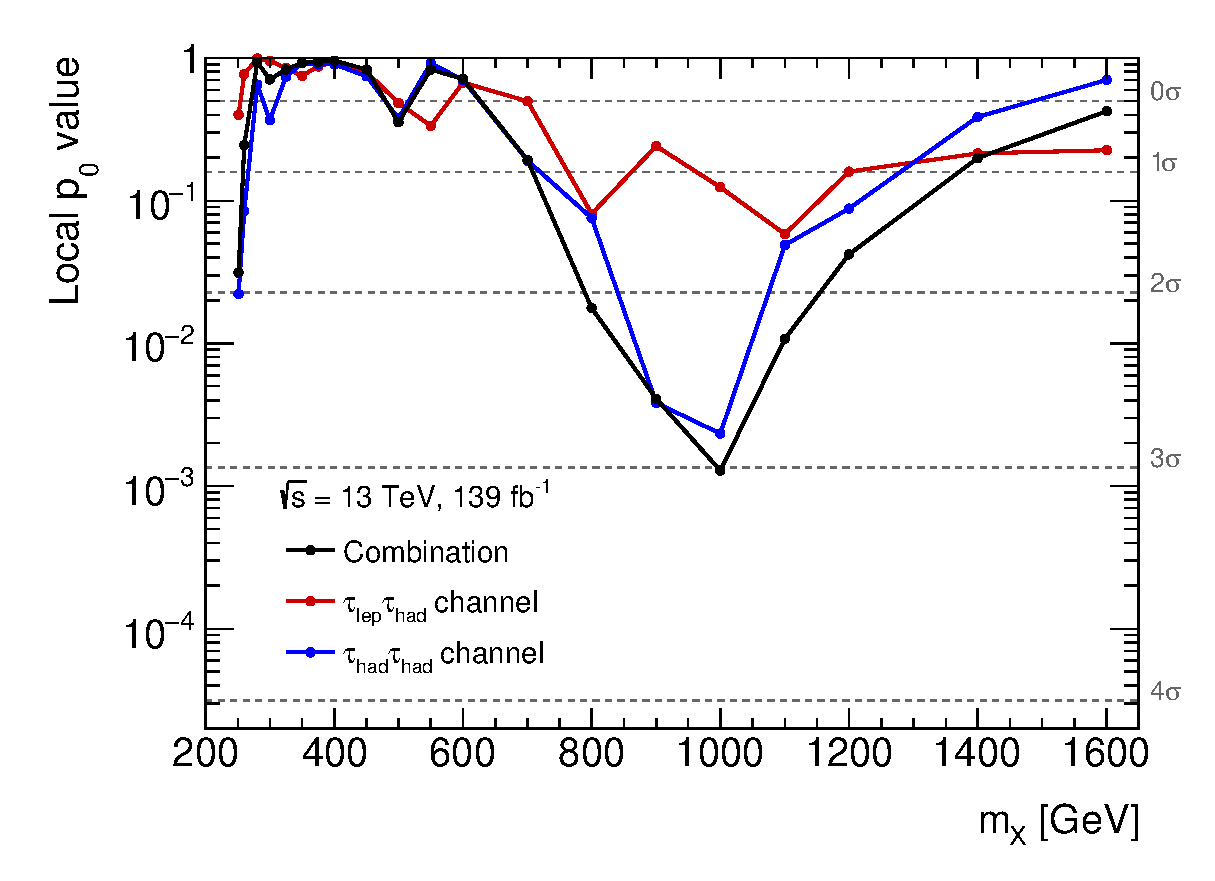
\includegraphics[width=0.65\textwidth]{results_res/resonant_comb_pvalues}

  \caption{Observed local $p$-values for the comparison of the background-only
    and the signal-plus-background model as a function of the mass of the scalar
    resonance. The asymptotic approximation of the sampling distribution of the
    discovery test statistic under the background-only model is used.}%
  \label{fig:local_pvalues}

  % Dashed lines indiciate the equivalent right-tailed probabilities in
  % terms of standard deviations of a centered Normal distribution,
  % formally given by the condition $p_0 = \mathbb{P}(Z > n \sigma)$
  % for~$Z \sim \mathcal{N}(0, \sigma^2)$ and $n = 0, 1, \dots, 4$.
  \todo[inline]{Discuss what's going on at 251? At around 400?}
\end{figure}

% Discuss the width of the excess
A broad excess can be observed in~\Cref{fig:local_pvalues} with tests of
resonances at masses in the range of \SIrange{800}{1200}{\GeV} being significant
at the $2\,\sigma$ level. At mass scales of \SI{1}{\TeV} a broad significance
response is expected for a true signal contribution due to the degradation in
absolute resolution of the \HH system mass and the lack of specificity of the
PNN discriminants in distinguishing between different signal hypotheses as
previously discussed in \Cref{sec:mva_pnn}. This effect is further illustrated
in \Cref{fig:local_pvalues_injected} where the observed local significances are
compared to the expectation after injecting signals at their best-fit signal
strengths. The width of significance response of the observed excess is similar
to the expectation obtained from these injection tests.

\begin{figure}[htbp]
  \centering

  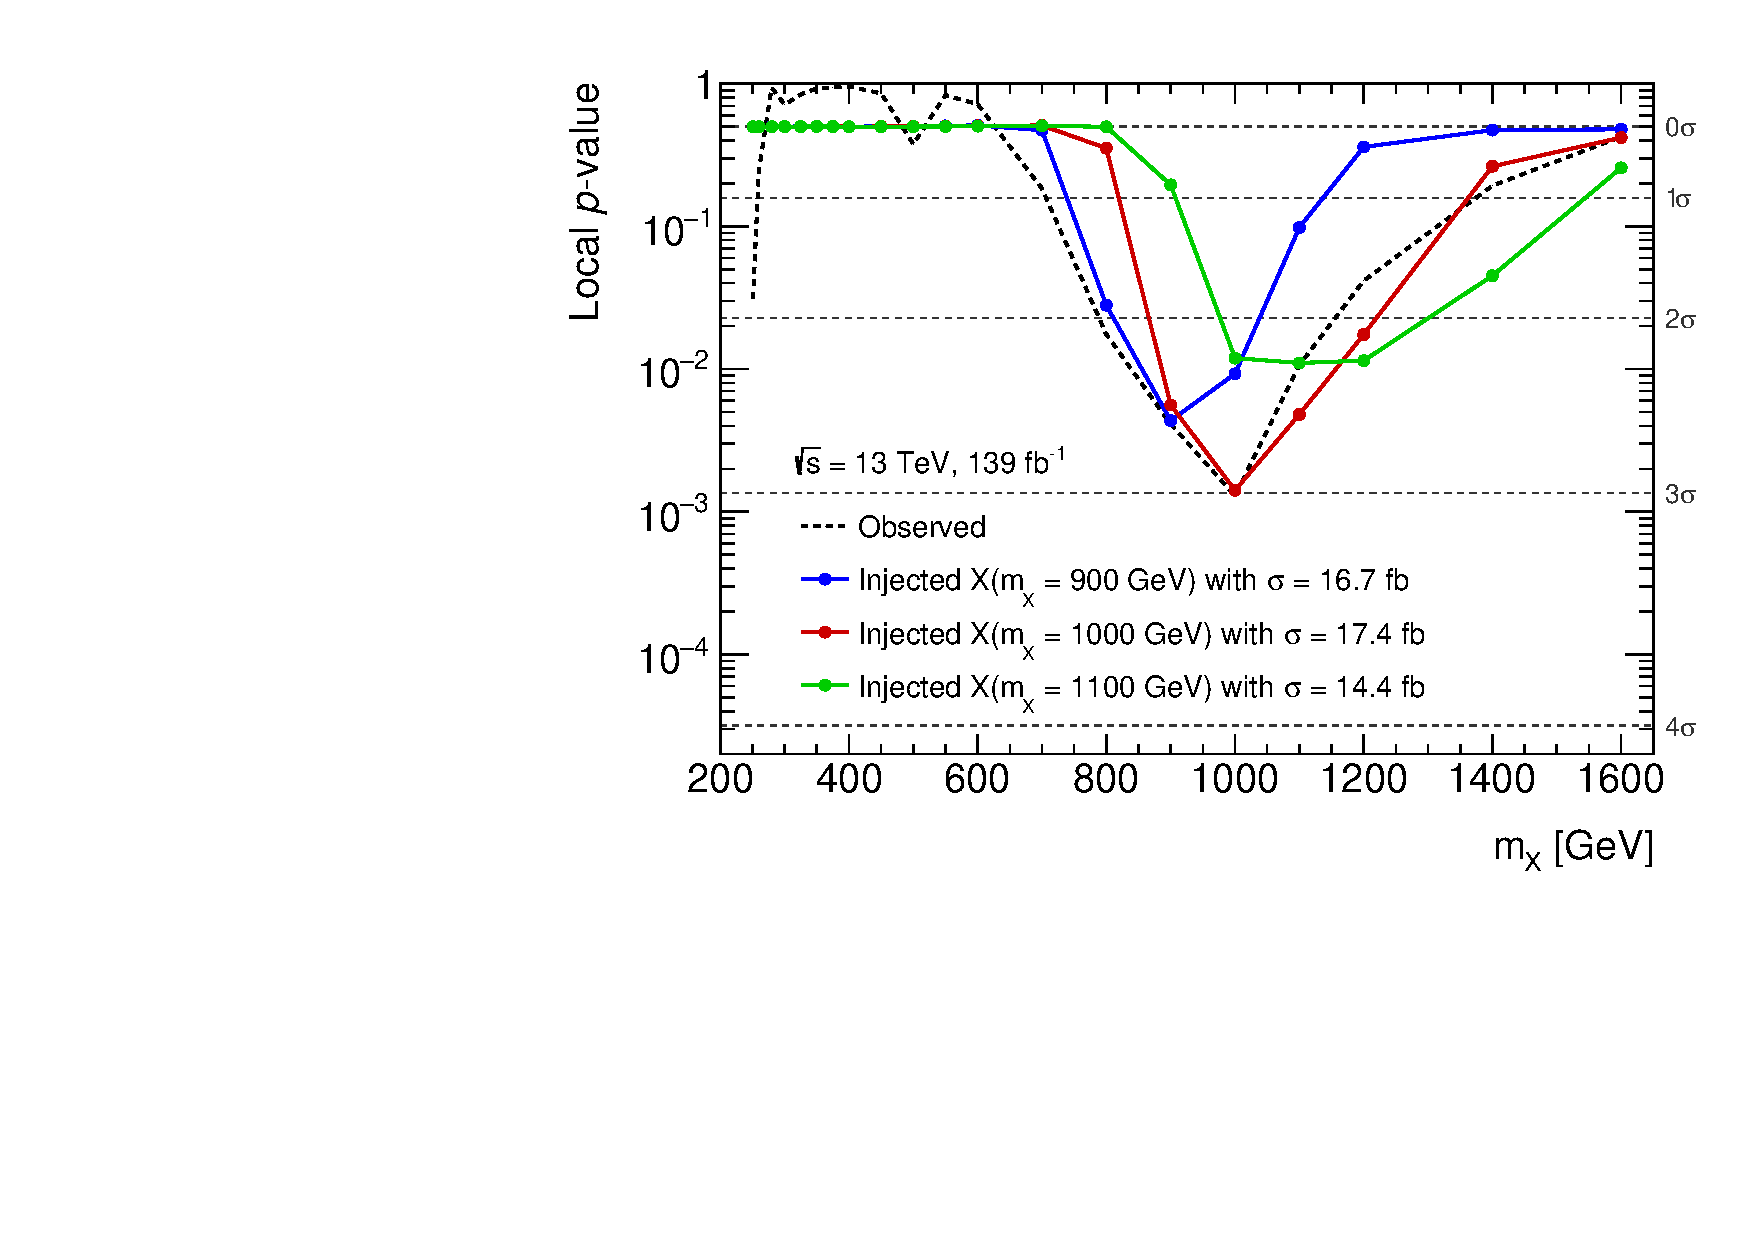
\includegraphics[width=0.65\textwidth]{results_res/injection}

  \caption{Expected local $p$-values from hypothesis tests performed on Asimov
    datasets with injected signals with \mX of 900, 1000, and
    \SI[group-minimum-digits=5]{1100}{\GeV}. The injected signals are normalised
    to their best-fit signal strength from the unconditional fit to observed
    data in all channels.  Signals are injected in all signal regions and the
    expected $p$-value resulting from the statistical interpretation of the
    combination of all channels is shown. Additionally, the observed $p$-values
    from the combination of all analysis channels (dashed line) are included for
    comparison.}
  \label{fig:local_pvalues_injected}
\end{figure}

The best-fit cross section of $pp \to X(\mX = \SI{1000}{\GeV}) \to HH$ obtained
from the fit of the PNN discriminants for $\mX = \SI{1000}{\GeV}$ to observed
data in all analysis channels is~\SIpmerr{17.4}{+7.5}{-6.5}{\femto\barn}. The
compatibility of the cross section measurement in the \hadhad and \lephad
channels is compared under the assumption of negligible correlation between the
measurements in both channels\footnote{The measurement is limited by the
  statistical precision of the number of observed events which are uncorrelated
  due to both channels being orthogonal.} yielding a significance of about
$1\sigma$. Therefore, the measurements in both channels, while some tension is
observed, are compatible. Further discussion of the nature of this excess will
be given in \Cref{sec:global_significance,sec:result_discussion}.

Upper limits are set on $\sigma(pp \to X \to \HH)$ as a function of the mass of
the scalar resonance, \mX, using the \CLs method at \SI{95}{\percent} confidence
level. The observed and expected exclusion limits on the cross section are shown
in \Cref{fig:res_upper_limits}. Scalar resonances produced with a cross sections
ranging from \SIrange{20}{900}{\femto\barn} depending on \mX are excluded given
the data observed in all analysis channels. The expected and observed limits are
additionally tabulated in~\Cref{app:limit_tables} for all \mX and separately for
the combination of all channels, \lephad-only, and \hadhad-only.

\begin{figure}[htbp]
  \centering

  % Workspaces: comb_2022_01_29
  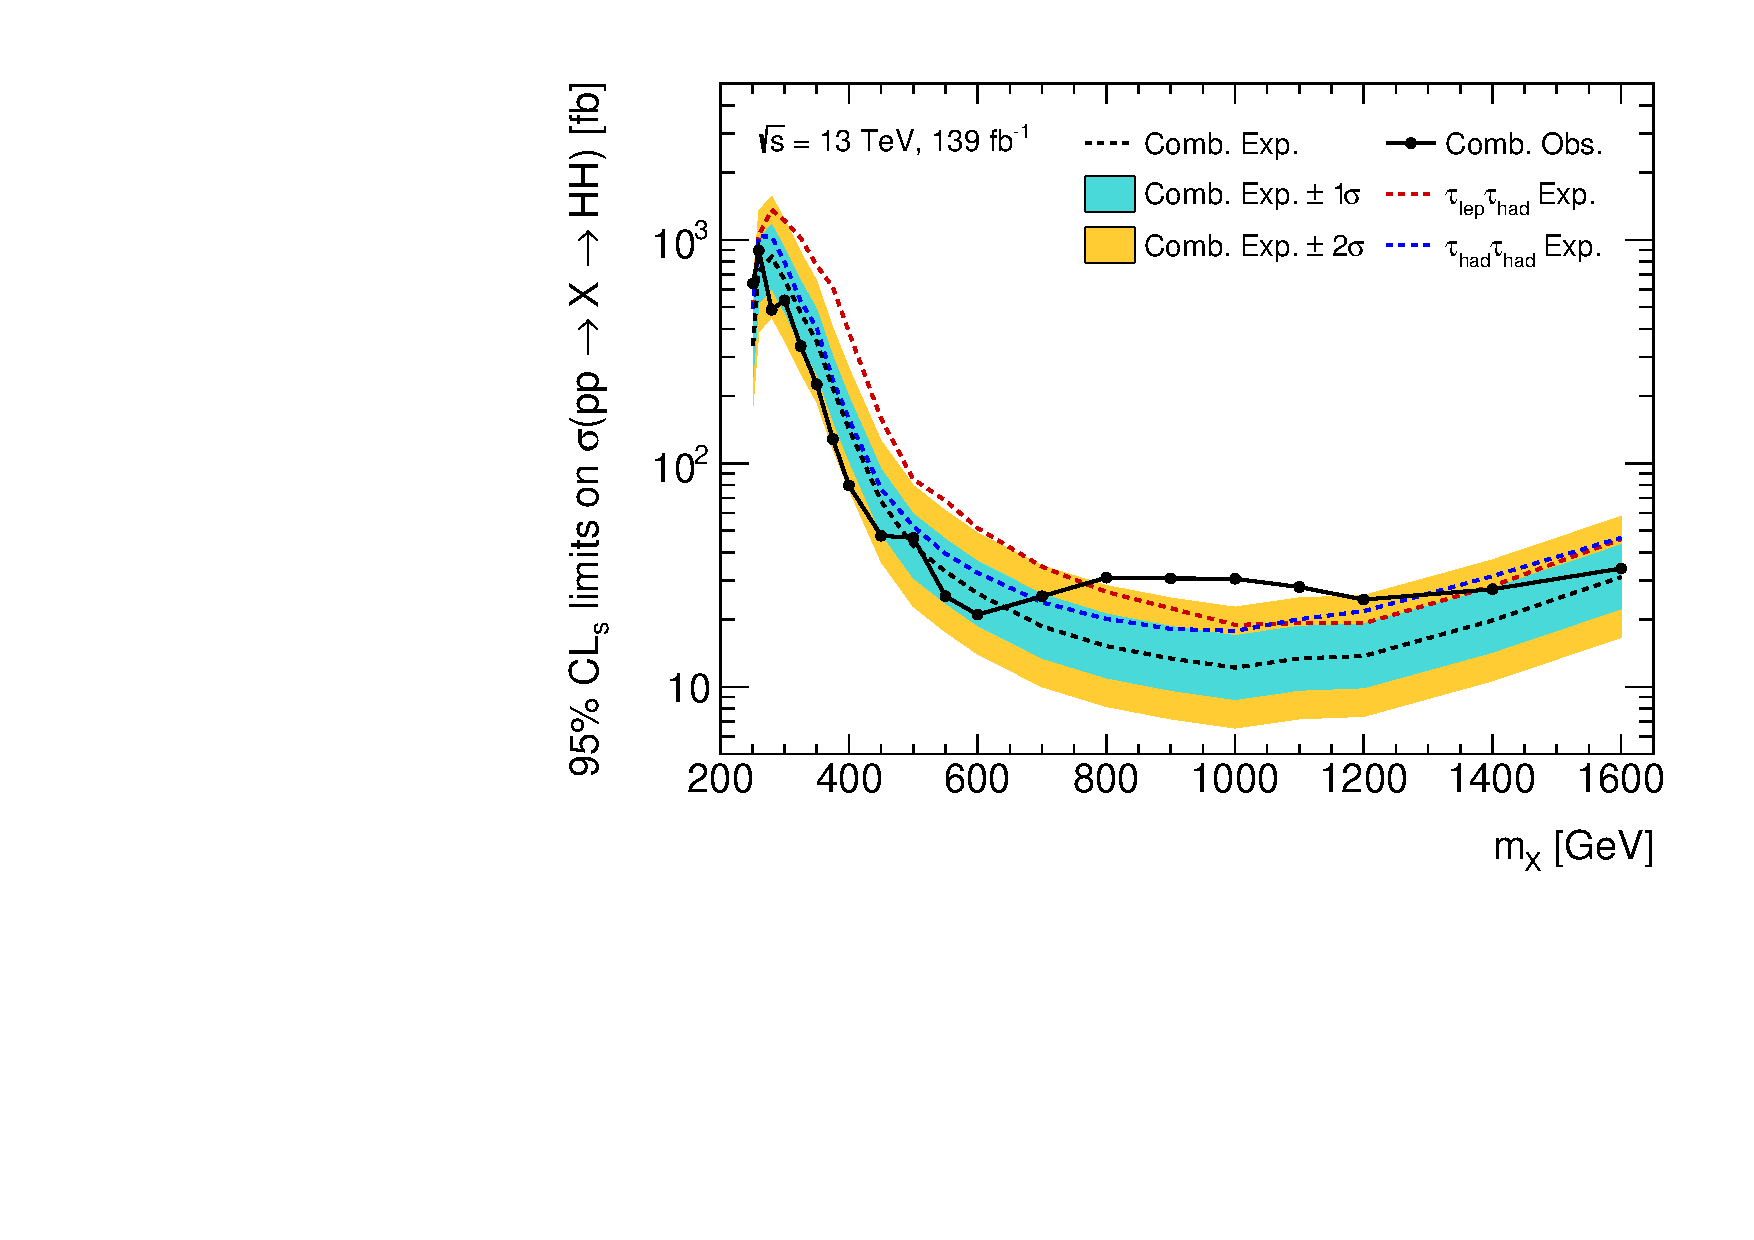
\includegraphics[width=0.65\textwidth]{results_res/resonant_upper_limits}

  \caption{Upper limits on $\sigma(pp \to X \to \HH)$ when considering different
    masses, \mX, of the scalar resonance. The exclusion limits are obtained
    using the asymptotic \CLs method at \SI{95}{\percent} confidence level. The
    expected upper limits obtained from tests of the \lephad and \hadhad channel
    only (incl.\ the control region) are overlayed to illustrate the sensitivity
    of individual channels.}%
  \label{fig:res_upper_limits}
\end{figure}

The upper limits on the cross section decrease quickly with increasing \mX in
the mass range from ca.\ \SIrange{300}{500}{\GeV}. This is a consequence of the
large positive slope in signal acceptance with respect to the mass of the scalar
resonance (cf.~\Cref{fig:signal_acceptance_resonant}) and the increasingly
distinct signature of the signal aiding in the discrimination between the signal
and background processes. Particularly the ability to distinguish the signal
from the top background, which has large contributions for
$\mX \lesssim \SI{500}{\GeV}$\todo{Yield tables for lephad would be nice},
increases quickly as larger resonance masses are considered. The signal
acceptance reaches a maximum at $\mX = \SI{1000}{\GeV}$ after which
reconstruction effects starts to degrade the acceptance due to the inability to
resolve the constituents of the $H \to \tautau$ and $H \to \bbbar$
candidates. This leads to a broad plateau of the upper limit and a degradation
of the exclusion limits at the upper end of the considered mass range.

The importance of individual analysis channels to the expected exclusion limit
varies as different resonance masses are considered. Except for the smallest \mX
considered, where the signal acceptance of the \hadhad channel is heavily
limited by the \tauhadvis-triggers, the \hadhad channel gives the most stringent
limits in the range of low to intermediate \mX due to the comparatively large
and irreducible top quark background in the \lephad channels. For hypotheses of
signal masses of about \SI{1000}{\GeV} and larger, the upper limits of both
channels start to converge since \Zjets production becomes the dominant
background in the most signal-like PNN bins at high \mX and the acceptance of
$Z \to \tautau + \text{jets}$ in both channels being similar\todo{Cross check
  this}.

The search for resonant production of Higgs boson pairs via scalar resonances is
primarily limited by the data statistical uncertainty particularly for
intermediate to high \mX. This is illustrated in~\Cref{tab:breakdown_res} where
the variance on the best-fit cross section from the unconditional
fit\footnote{The excess for $\mX = \SI{1000}{\GeV}$ induces shifts in the
  (observed) variance breakdown depicted in~\Cref{tab:breakdown_res}, slightly
  inflating data statistical uncertainties while suppressing the impact of most
  systematic uncertainties (the exception being signal modelling uncertainties)
  compared to the
  expectation. In~\Cref{app:breakdown_table}~\Cref{tab:breakdown_res_exp_mu0}
  the decomposition is performed for the expectation of
  $\sigma(pp \to X \to HH) = 0$ for comparison.}, $\hat{\sigma}$, is decomposed
into categories of uncertainties for four exemplary signal mass hypotheses.

\begin{table}[htbp]
  \centering

  \caption{Decomposition of the variance on $\hat{\sigma}$, the maximum
    likelihood estimate of the cross section $\sigma(pp \to X\to HH)$, by
    uncertainty category for the fit to observed data in all regions. The
    decomposition is determined analogously to~\Cref{tab:breakdown_nonres},
    separately for four exemplary signal mass hypotheses. The fractions of
    subcategories do not necessarily sum to the fraction of the parent category
    due to correlations between nuisance parameters.}%
  \label{tab:breakdown_res}

  % Observed breakdown
  \begin{tabular}{
  l
  S[table-format=2.0, table-space-text-pre=\textless, table-column-width=1.6cm]
  S[table-format=2.0, table-space-text-pre=\textless, table-column-width=1.6cm]
  S[table-format=2.0, table-space-text-pre=\textless, table-column-width=1.6cm]
  S[table-format=2.0, table-space-text-pre=\textless, table-column-width=1.6cm]
  }
  \toprule
         & \multicolumn{4}{c}{Explained fraction of variance on $\hat{\sigma}$}\\
         %& \multicolumn{4}{c}{of variance on $\hat{\mu}$}\\
  \cmidrule{2-5}
  Source & {$\SI{300}{\GeV}$} & {$\SI{500}{\GeV}$} & {$\SI{1000}{\GeV}$} & {$\SI{1600}{\GeV}$} \\
  \midrule
  \textbf{Data statistical uncertainty}
         & 58\,\si{\percent} & 81\,\si{\percent} & 86\,\si{\percent} & 82\,\si{\percent} \\
  \textbf{Systematic uncertainties}
         & 42\,\si{\percent} & 19\,\si{\percent} & 14\,\si{\percent} & 18\,\si{\percent} \\
  \hspace{0.8em} Instrumental uncertainties
         & 10\,\si{\percent} & 1\,\si{\percent} & 2\,\si{\percent} & {\textless} 1\,\si{\percent}\\
  \hspace{0.8em} Signal modelling uncertainties
         & 2\,\si{\percent}  & 1\,\si{\percent} & 2\,\si{\percent} & 3\,\si{\percent} \\
  \hspace{0.8em} Background statistical uncertainties
         & 19\,\si{\percent} & 11\,\si{\percent} & 3\,\si{\percent} & 11\,\si{\percent} \\
  \hspace{0.8em} Background modelling uncertainties
         & 14\,\si{\percent} & 6\,\si{\percent} & 7\,\si{\percent} & 4\,\si{\percent} \\
  \midrule
  \hspace{1.6em} -- \hspace{0.2em} Top-quark (incl.\ free normalisation)
         & 3\,\si{\percent} & 2\,\si{\percent} & 1\,\si{\percent} & {\textless} 1\,\si{\percent} \\
  \hspace{1.6em} -- \hspace{0.2em} \ZHF (incl.\ free normalisation)
         & 4\,\si{\percent} & 1\,\si{\percent} & 2\,\si{\percent} & 1\,\si{\percent} \\
  \hspace{1.6em} -- \hspace{0.2em} SM Higgs boson
         & {\textless} 1\,\si{\percent} & 2\,\si{\percent} & 2\,\si{\percent} & 2\,\si{\percent} \\
  \hspace{1.6em} -- \hspace{0.2em} Fake-\tauhadvis
         & 4\,\si{\percent} & {\textless} 1\,\si{\percent} & 1\,\si{\percent} & {\textless} 1\,\si{\percent} \\
  \hspace{1.6em} -- \hspace{0.2em} Other
         & {\textless} 1\,\si{\percent} & {\textless} 1\,\si{\percent} & {\textless} 1\,\si{\percent} & {\textless} 1\,\si{\percent} \\
  \bottomrule
\end{tabular}

%%% Local Variables:
%%% mode: latex
%%% TeX-master: "../phd_thesis"
%%% End:


  % Expected breakdown for Asimov with mu = 0
  % \begin{tabular}{
  l
  S[table-format=2.0, table-space-text-pre=\textless, table-column-width=1.6cm]
  S[table-format=2.0, table-space-text-pre=\textless, table-column-width=1.6cm]
  S[table-format=2.0, table-space-text-pre=\textless, table-column-width=1.6cm]
  S[table-format=2.0, table-space-text-pre=\textless, table-column-width=1.6cm]
  }
  \toprule
         & \multicolumn{4}{c}{Explained fraction of variance on $\hat{\sigma}$}\\
         %& \multicolumn{4}{c}{of variance on $\hat{\mu}$}\\
  \cmidrule{2-5}
  Source & {$\SI{300}{\GeV}$} & {$\SI{500}{\GeV}$} & {$\SI{1000}{\GeV}$} & {$\SI{1600}{\GeV}$} \\
  \midrule
  \textbf{Data statistical uncertainty}
         & 59\,\si{\percent} & 81\,\si{\percent} & 82\,\si{\percent} & 82\,\si{\percent} \\
  \textbf{Systematic uncertainties}
         & 41\,\si{\percent} & 19\,\si{\percent} & 18\,\si{\percent} & 17\,\si{\percent} \\
  \hspace{0.8em} Instrumental uncertainties
         & 10\,\si{\percent} & 1\,\si{\percent} & 1\,\si{\percent} & {\textless} 1\,\si{\percent}\\
  \hspace{0.8em} Signal modelling uncertainties
         & 1\,\si{\percent}  & 1\,\si{\percent} & {\textless} 1\,\si{\percent} & 3\,\si{\percent} \\
  \hspace{0.8em} Background statistical uncertainties
         & 18\,\si{\percent} & 11\,\si{\percent} & 7\,\si{\percent} & 9\,\si{\percent} \\
  \hspace{0.8em} Background modelling uncertainties
         & 12\,\si{\percent} & 7\,\si{\percent} & 10\,\si{\percent} & 5\,\si{\percent} \\
  \midrule
  \hspace{1.6em} -- \hspace{0.2em} Top-quark (incl.\ free normalisation)
         & 3\,\si{\percent} & 2\,\si{\percent} & 1\,\si{\percent} & {\textless} 1\,\si{\percent} \\
  \hspace{1.6em} -- \hspace{0.2em} \ZHF (incl.\ free normalisation)
         & 3\,\si{\percent} & 1\,\si{\percent} & 3\,\si{\percent} & 2\,\si{\percent} \\
  \hspace{1.6em} -- \hspace{0.2em} SM Higgs boson
         & {\textless} 1\,\si{\percent} & 2\,\si{\percent} & 3\,\si{\percent} & 2\,\si{\percent} \\
  \hspace{1.6em} -- \hspace{0.2em} Fake-\tauhadvis
         & 4\,\si{\percent} & {\textless} 1\,\si{\percent} & 1\,\si{\percent} & 1\,\si{\percent} \\
  \hspace{1.6em} -- \hspace{0.2em} Other
         & {\textless} 1\,\si{\percent} & {\textless} 1\,\si{\percent} & {\textless} 1\,\si{\percent} & {\textless} 1\,\si{\percent} \\
  \bottomrule
\end{tabular}

%%% Local Variables:
%%% mode: latex
%%% TeX-master: "../phd_thesis"
%%% End:

\end{table}

Systematic uncertainties have a sizeable effect on the total variance of
$\hat{\sigma}$ only for searches of scalar resonances with low
mass. Instrumental uncertainties, most significantly uncertainties affecting
jets / \pTmissAbs and \tauhadvis, have the largest impact on the search when the
final state objects constituting the Higgs boson candidates are produced with
low transverse momenta, which is typically the case for signals with small
\mX. Similarly, \faketauhadvis backgrounds and uncertainties related to their
data-driven estimation, which are partially included in the background
statistical uncertainties due to the finite number events in the control regions
(and non-multi-jet subtraction in the case of the \hadhad channel), play a more
significant role at low \mX.


\todo[inline]{Ranking plots: Selected masses combined only?}

\todo[inline]{Table of lephad yields?}

\subsection{Estimation of the Global Significance for the Excess at
  $\mX = \SI{1000}{\GeV}$}%
\label{sec:global_significance}

\todo[inline]{Note that this focuses on the combination of all
  channels.}

In the search for resonant Higgs boson pair production multiple hypothesis tests
are performed that probe for 20 different \mX of the scalar resonance. The
previously quoted significance of $3.0\,\sigma$ of the test at
$\mX = \SI{1000}{\GeV}$ does not account for the effect of multiple hypothesis
testing and was therefore referred to as the local significance. Under the
background-only hypothesis, any of the 20 tests could yield a statistically
significant result by chance, possibly leading to a false
discovery.\footnote{This concept is usually referred to as the look-elsewhere
  effect in HEP.}

Formally, the effect of multiple testing can be accounted for by considering the
probability to make one or more false discoveries (type II errors) when
considering an entire family of hypothesis tests.
% and the associated critical thresholds on the test statistics.
This probability, which is referred to as the family-wise error rate (FWER), can
be controlled by setting the critical thresholds of the tests
appropriately. When accounting for the effect of multiple testing in searches
for new physics, all hypothesis tests are usually treated equally resulting in
the same thresholds being applied in all tests. By convention in HEP, the
critical thresholds are not adjusted explicitly to control the FWER but rather
the FWER corresponding to the threshold equal to the observed test statistic of
the most significant test is given directly. In this case the FWER is
\begin{align*}
  \pglobal = \text{FWER}(\zmaxlocal)
  = \mathbb{P}(\Zmaxlocal > \zmaxlocal \vert H_0)\,\text{,}
\end{align*}\todo{Define directly via the probability to observe an excess larger than the observed one.}
where \zmaxlocal is the observed maximum of the local significance and
\Zmaxlocal the random variable describing the maximum local significance under
the background-only hypothesis ($H_0$). In both cases the maximum is taken over
the family of hypothesis tests considered in the statistical interpretation.

\todo[inline]{Say that in all cases we assume the background-only hypothesis
  unless otherwise noted.}

This formulation %of the FWER
is equivalent to the $p$-value of a hypothesis test that employs the maximum
local significance over a family of tests as the test statistic and observing
$\Zmaxlocal = \zmaxlocal$, and is thus called the global $p$-value or \pglobal
for brevity. This global $p$-value is subsequently translated into the global
significance, analogously to the treatment of local $p$-values and
significances, according to
\begin{align*}
  z_{\text{global}} = \Phi^{-1}(1 - \pglobal) \,\text{,}
\end{align*}
where $\Phi^{-1}$ is the quantile function of the Standard Normal distribution.

In practice the global significance can be determined using simulation provided
a probabilistic model of $H_0$ is available. A number of $N$ toy experiments can
be drawn from $H_0$, subsequently performing the set of hypothesis tests on all
experiments and noting, separately for every toy experiment, the maximum local
significance over all tests, \zmaxlocal. The global $p$-value is then estimated
as the fraction of toy experiments with \zmaxlocal exceeding the observed value
\begin{align*}
  \pglobal \approx \frac{ \text{Number of toys with } \zmaxlocal > z_{\text{local, obs}}^{\text{max}} }
                        { N } \,\text{,}
  %= \mathbb{E} ( \mathbf{1}_{[z, \infty)}(\zmaxlocal) \vert H_0 )
  %\approx \frac{1}{N} \sum_{i = 1}^N \mathbf{1}_{[z, \infty)}\left( \zmaxlocal_{, i} \right)
\end{align*}
where $z_{\text{local, obs}}^{\text{max}}$ refers to the observed maximum local
significance in data. Other methods for calculating global significances exist,
see for example Ref.~\cite{Gross:2010qma}, that generally also rely on the
ability of drawing toy experiments from $H_0$.

The primary difficulty in estimating the global significance of the excess at
$\mX = \SI{1000}{\GeV}$ lies in the generation of toy experiments from the
background-only hypothesis. While the likelihood functions used for the
statistical interpretation contain a model of the binned PNN discriminants,
these models only provide a description of a single discriminant at a time, not
accounting for dependencies between observables of different discriminants. The
estimation of the global significance, however, requires a background model
jointly describing all binned discriminants used in the search, which is not
readily available.

The need for such a joint model was already indicated by the large width of the
significance response in the signal injection tests for large \mX
(cf.~\Cref{fig:local_pvalues_injected}) which is caused by a partial overlap of
signal events in the most signal-like bins of PNN discriminants for adjacent
mass points. This overlap is expected to extend to background events and thus
will have an effect on the global significance estimation which has to be
quantified.

A substitute background model is constructed, accounting for correlations
between all observables entering the statistical interpretation, that can be
used to generate toy experiments for the global significance estimation. This
model should closely approximate the marginal models contained in the likelihood
functions (i.e.\ the model of a single binned PNN discriminant) such that the
statistical analysis can proceed using the same likelihood functions without
incurring large biases due to a mismatch between models.

The model is constructed assuming the pre-fit expectation for all backgrounds,
except for the normalisation factors of the \ttbar and \ZHF backgrounds, which
are set to approximate post-fit values of 0.97 and 1.35, respectively. Two major
classes of random variables need to be considered when generating toy
experiments:
\begin{enumerate}
\item Random variables describing the observed number of events in a given bin,
  usually referred to as \emph{observables}.

\item Random variables describing the central value of auxiliary measurements
  that provide the description of systematic uncertainties. These are referred
  to as \emph{global observables}.
\end{enumerate}

\emph{Observables} are expected to be partially correlated due to the overlap of
events between pairs of bins of different PNN discriminants. Their treatment
will be discussed in the following section.

\emph{Global observables} need to be further subdivided into two cases. First,
the global observables related to the auxiliary measurement encoding the
statistical uncertainty on the background
estimate %(due to the finite number of simulated events and events in
% the control region)
according to the Barlow-Beeston method. Second, all other global observables
describing experimental and theory uncertainties. The latter are assumed to be
fully correlated for all hypothesis tests performed in this search, while the
former are also partially correlated due to an overlap of simulated / control
region events between bins. The treatment of global observables will be
discussed in a later section.

The generation of random variates for observables, and global observables
related to the Barlow-Beeston method can proceed independently for all analysis
channels due to their orthogonality. Standard procedures are used in the control
region to generate these random variates since the contribution of this region
to the likelihood functions is identical for all tests.

%Driven by data statistics. But MC background statistical uncertainties
%are non-negligible.

\subsubsection{Generation of Toy Observables}

For the generation of random toy observables, the correlation between
observables based on the overlap of bins needs to be quantified. Let $A$ and $B$
be observables corresponding to a pair of bins which are marginally distributed
according to Poisson distributions. The dependence between $A$ and $B$ is given
by the overlap in the kinematic region (phase space) selected by both bins. The
phase space selected by either bin can be partitioned into three parts with
associated observables $X_i$:
\begin{itemize}
\item The phase space selected by bin A but not B with observable $X_1$.
\item The phase space selected by bin A and B with observable $X_2$.
\item The phase space selected by bin B but not A with observable $X_3$.
\end{itemize}
Due to the partitioning of the phase space, the observables $X_i$ are i.i.d.\
$\pois(\lambda_i)$ with rate parameters $\lambda_i$ for $i = 1, 2, 3$. The
observables $A$ and $B$ can thus be written as
\begin{align*}
  A &= X_1 + X_2 \sim \pois(\lambda_1 + \lambda_2) \\
  B &= X_2 + X_3 \sim \pois(\lambda_2 + \lambda_3)
\end{align*}
and the Pearson correlation coefficient between $A$ and $B$ can be determined
as\footnote{$\cov(A,B) = \cov(X_1 + X_2, X_2 + X_3) = \cov(X_2, X_2) = \var(X_2)
  = \lambda_2$ from the independence of $X_1$, $X_2$, and $X_3$.}
\begin{align*}
  \rho_{AB} = \frac{\cov(A, B)}{\sqrt{\var(A)\var(B)}}
  = \frac{\lambda_2}{\sqrt{(\lambda_1 + \lambda_2) \cdot (\lambda_2 + \lambda_3)}} \,\text{,}
\end{align*}
which reflects the intuition that the overlap in selected phase space, described
by the rate $\lambda_2$, induces a correlation between both observables. In the
following, the model described by $A$ and $B$ will be referred to as the
bivariate Poisson model.

An approximation of the correlation coefficient for all pair-wise combinations
of bins in an analysis channel can be obtained by replacing the rate parameters
$\lambda_i$ by the rates from the background estimate. Submatrices of the
correlation matrix obtained in the \hadhad channel are shown
in~\Cref{fig:correlation_matrix_observables}. A total of 144 bins from the
\hadhad channel enter the statistical interpretation leading to a matrix of
dimension $144 \times 144$. Similar matrices are obtained in the \lephad SLT and
LTT signal regions with dimension $193 \times 193$ and $182 \times 182$,
respectively.

\begin{figure}[htbp]
  \centering

  \begin{subfigure}{\textwidth}
    \centering

    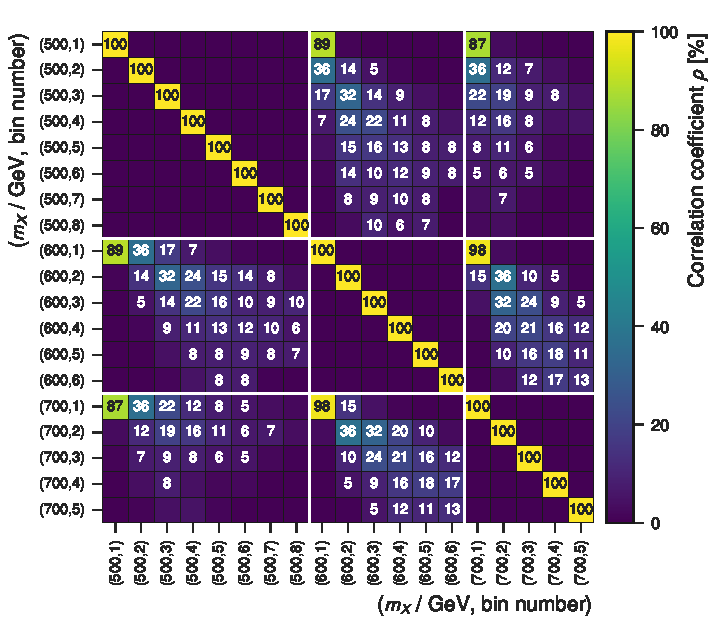
\includegraphics[scale=0.8]{global_significance/observable_correlations/corr_hadhad_medium}
    \subcaption{Submatrix for observables of
      $\mX = 500, 600, 700\,\si{\GeV}$ discriminants}%
    \label{fig:correlation_matrix_observables_medium}
  \end{subfigure}

  \begin{subfigure}{\textwidth}
    \centering

    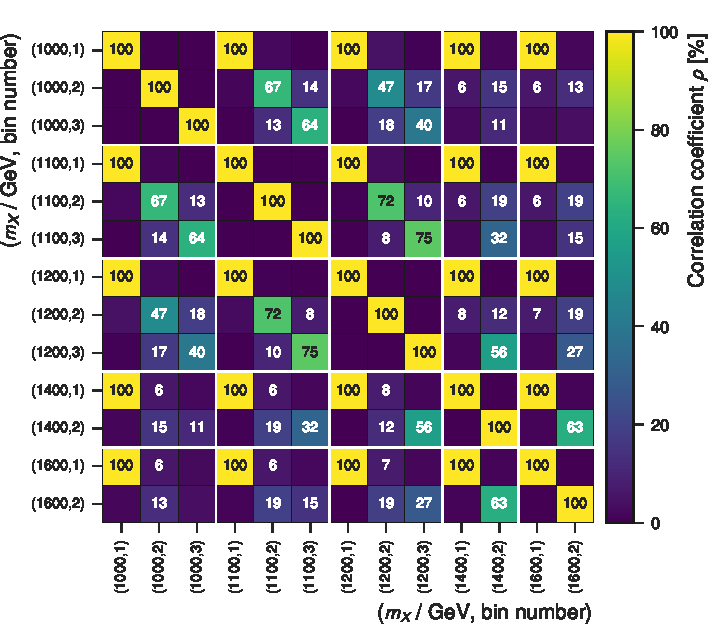
\includegraphics[scale=0.8]{global_significance/observable_correlations/corr_hadhad_high}
    \subcaption{Submatrix for observables of
      $\mX = 1000, 1100, 1200, 1400, 1600\,\si{\GeV}$ discriminants}%
    \label{fig:correlation_matrix_observables_high}
  \end{subfigure}

  \caption{Estimate of the correlation matrix between observables of \hadhad
    channel. Two submatrices of the full matrix ($144 \times 144$) are
    shown. Bins are enumerated in ascending order of the signal probability
    according to the PNN discriminants (i.e.\ bins numbered with 1 contain the
    most background-like events for a given classification problem).  Cells are
    annotated if the correlation coefficient is larger than or equal to
    \SI{5}{\percent}. Off-diagonal elements with a correlation coefficient of
    \SI{100}{\percent} are due to rounding only.}%
  \label{fig:correlation_matrix_observables}
\end{figure}

\Cref{fig:correlation_matrix_observables_medium} shows estimated correlation
coefficients between observables of discriminants used to select signals from
resonances in the intermediate mass range in the \hadhad channel. This
correlation matrix has some noteworthy features:
\begin{itemize}
\item Off-diagonal elements of submatrices describing the correlation of
  observables belonging to the same PNN discriminant are zero due to bins being
  disjoint by construction.

\item The most background-like bins (i.e.\ bins enumerated with 1) have
  correlation coefficients of about \SI{90}{\percent} or larger. This is due to
  the presence of events that are easily rejected by the PNN discriminants,
  which predominately populate the first bins. A correlation in such bins is
  expected, independent of the targeted \mX, due events being selected that are
  kinematically incompatible with resonant Higgs boson pair production. An
  example for such events are the ones where both \mMMC and \mBB are far from
  \mH.

\item The observables of the most signal-like bins are expected to have little
  correlation for the three PNN discriminants targeting the intermediate mass
  range considered in~\Cref{fig:correlation_matrix_observables_medium}.
  % The signal extraction procedure has sufficient mass
  % resolution to distinguish between signal hypotheses in the
  % intermediate mass range.
\end{itemize}

The expected correlation between observables of the high \mX discriminants are
shown in~\Cref{fig:correlation_matrix_observables_high} for the \hadhad
channel. As previously noted, the signal extraction method is unable to separate
the signatures of signal-like events at high \mX. This is reflected in the
correlation coefficient of the observables for the most signal-like bins of
adjacent mass points reaching values of up to \SI{75}{\percent}. The correlation
matrices estimated for the \lephad SLT and LTT channels yield similar
results\todo{Put in appendix?}.

Considering these dependencies between observables, the toy generation for the
purpose of estimating the global significance needs to fulfil certain
requirements. First, the model needs to accurately reproduce the marginal
distributions of the observables, i.e.\ Poisson distributions with rates given
by the background estimate, such that the distribution of the discovery test
statistic for individual tests at fixed \mX can be reproduced. Second, it needs
to model the dependence structure between observables to account for the overlap
of phase space selected by the bins entering the statistical interpretation.

A multivariate extension of the bivariate Poisson distribution would fulfil
these requirements, however, such a model becomes intractable due to the large
number of observables considered, and in particular due to the presence of
negatively weighted events used for the background estimate.\footnote{In the
  absence of negatively weighted events, toy experiments could be generated
  using pseudo-data generated by drawing a random weight from $\pois(w_i)$ for
  every event with weight $w_i$ used for the background estimate. Subsequently,
  the set of pseudo-data can be used to determine the values of all
  observables. Conceptually, this approach has some parallels to resampling
  techniques like the Bootstrap
  method~\cite{10.1214/aos/1176344552,efron1994introduction}.} Instead, a model
based on the mathematical framework provided by Sklar's
theorem~\cite{Sklar1959FonctionsDR} is adopted, allowing to factorise the
marginal distributions from the dependency structure of the observables.

Sklar's theorem states~\cite{nelsen} that any $n$-dimensional joint distribution
function $H$ can be decomposed into its marginal distribution functions
$F_1, \dots, F_n$ and an $n$-dimensional copula $\mathcal{C}$. The copula
$\mathcal{C}$ is an $n$-dimensional distribution function,
$\mathcal{C}: [0, 1]^n \rightarrow [0, 1]$, with uniform marginal densities that
describes the dependencies between random variables.\footnote{The copula is
  uniquely identifiable for continuous marginals, however, this is not the case
  for discrete marginal distributions.} The joint distribution can thus be
expressed as
\begin{align*}
  H(x_1, \dots, x_n) = \mathcal{C}(F_1(x_1), \dots, F_n(x_n))
\end{align*}
according to the theorem.

For the task of generating toy experiments, the only missing piece is the
functional form of the copula since the marginal distributions are assumed to be
known from the nominal background prediction. The Poisson distribution can be
approximated by a Normal distribution provided the expected rate is not too
small, suggesting that the copula describing the dependence structure of a
multivariate Normal distribution might be applicable as an approximation. This
copula, referred to as the Gaussian copula, can be derived using the inversion
method described in Ref.~\cite{nelsen} and is given by
\begin{align}
  \label{eq:gaussian_copula}
  \mathcal{C}_{\myvec{R}}(u_1, \dots, u_n) = \Phi_{\myvec{R}}(\Phi^{-1}(u_1), \dots, \Phi^{-1}(u_n))
\end{align}
where $\Phi_{\myvec{R}}$ is the CDF of the multivariate Normal distribution with
zero mean and covariance equal to the correlation matrix~$\myvec{R}$, and
$\Phi^{-1}$ is the quantile function of the univariate Standard Normal
distribution. Similar approaches of modelling multivariate count data using
copulas have been explored in Refs.~\cite{10.1002/wics.1398}\todo{Add more
  references}.

The parameters $\myvec{R}$ of the Gaussian copula are estimated using the
correlation matrices derived with the bivariate Poisson model previously shown
in~\Cref{fig:correlation_matrix_observables}. The modelling assumptions are
investigated empirically in two dimensions using comparisons of simulated
results for the bivariate Poisson model and the copula-based model. The
dependence of two observables $A$ and $B$ is illustrated in
\Cref{fig:copula_model_comparison} for both models in terms of the conditional
mean and variance of $B$ given the observation $A = a$. This comparison is
performed, instead of a direct comparison of joint distribution functions, to
better illustrate the subtle differences between both models. The comparison
yields the following findings:
\begin{itemize}
\item The conditional mean of $B$ given $A = a$ agrees well between models even
  when considering bin pairs with the lowest rates $\lambda_i$ relevant for the
  analysis. This agreement is not unexpected since the Pearson correlation
  coefficient used to define the model is linked to the slope of the regression
  line that predicts $\mathrm{E}(B \vert A = a)$.

\item The conditional variance of $B$ given $A = a$ illustrates that both models
  are not equivalent, however. For bin pairs with small expected rates
  $\lambda_i$, the variance of the distribution of $B$ for fixed $A = a$ differs
  by up \SI{15}{\percent} to between both models. These deviations are assumed
  to be negligible compared to the linear trend that is properly captured by the
  model.

\item In the case of disjoint or fully overlapping\footnote{The case of fully
    overlapping bins requires special treatment since the correlation matrix
    would be singular.} bins (not shown in the figure) the bivariate Poisson
  model and copula-based model are identical.
\end{itemize}

\begin{figure}[htbp]
  \centering

  \begin{subfigure}{\textwidth}
    \centering
    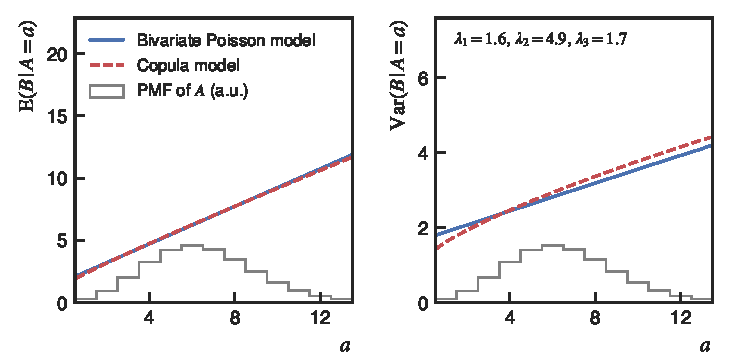
\includegraphics[scale=0.9]{global_significance/model_comparison/comparison_example_1}
    \subcaption{Most signal-like bins of the $\mX = \SI{1100}{\GeV}$
      and $\mX = \SI{1200}{\GeV}$ discriminants
      ($\rho = \SI{75}{\percent}$).}
  \end{subfigure}

  \begin{subfigure}{\textwidth}
    \centering
    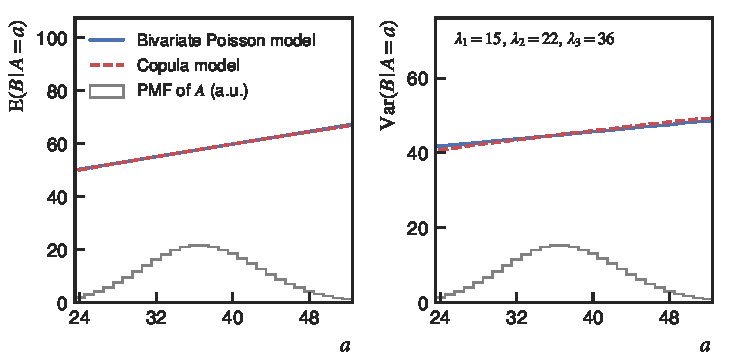
\includegraphics[scale=0.9]{global_significance/model_comparison/comparison_example_3}
    \subcaption{Second bin of the $\mX = \SI{1000}{\GeV}$ and second
      bin of the $\mX = \SI{1200}{\GeV}$ discriminant
      ($\rho = \SI{47}{\percent}$).}
  \end{subfigure}

  \begin{subfigure}{\textwidth}
    \centering
    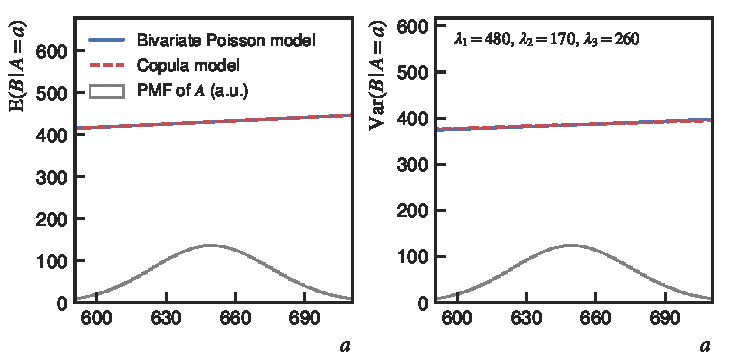
\includegraphics[scale=0.9]{global_significance/model_comparison/comparison_example_4}
    \subcaption{Third bin of the $\mX = \SI{500}{\GeV}$ and second bin
      of the $\mX = \SI{600}{\GeV}$ discriminant
      ($\rho = \SI{32}{\percent}$).}
  \end{subfigure}

  \caption{Comparison of the bivariate Poisson model and the copula model with a
    Gaussian copula specified by
    $\rho = \lambda_2 / \sqrt{(\lambda_1 + \lambda_2) \cdot (\lambda_2 +
      \lambda_3)}$ and marginal distributions given by
    $A \sim \pois(\lambda_1 + \lambda_2)$ and
    $B \sim \pois(\lambda_2 + \lambda_3)$. The conditional mean (left panels)
    and variance (right panels) of $B$ given the observation $A = a$ is shown to
    illustrate the dependence of both random variables. Three different
    scenarios are shown varying in the expected rates $\lambda_i$ and in the
    correlation coefficients $\rho$ between $A$ and $B$. The scenarios are
    chosen from bin pairs for the \hadhad channel discriminants.  The
    probability mass function (PMF) of $A$ is overlayed in arbitrary units
    (a.u.).}%
  \label{fig:copula_model_comparison}
\end{figure}

With these simplifying modelling assumptions, observables can be randomly
generated using the multivariate copula-based model. The following algorithm
allows to draw the vector of random variates $\myvec{x} = (x_1, \dots, x_n)$
from the joint distribution described by the Gaussian copula and marginal
distributions:
\begin{enumerate}
\item Draw a vector of random variates, $\myvec{u} = (u_1, \dots, u_n)$, from
  the distribution described by $\mathcal{C}_{\myvec{R}}$.

  The vector $\myvec{u}$ is obtained by generating random variates
  $\myvec{n} = (n_1, \dots, n_n)$ from the centred multivariate Normal
  distribution with covariance matrix equal to $\myvec{R}$, followed by an
  element-wise application of the univariate Standard Normal CDF to $\myvec{n}$,
  i.e.\ $u_i = \Phi(n_i)$ for every $i = 1, \dots, n$. This procedure follows
  directly from the form of the Gaussian copula in~\Cref{eq:gaussian_copula}.

  In practice, the matrices $\myvec{R}$ that are considered here are singular
  due to multicollinearity between observables. This arises from 19 implicit
  constraints due to the requirement that the sum of observables is the same for
  all 20 discriminants in a given analysis channel, thus leading to 19 vanishing
  eigenvalues of $\myvec{R}$. Therefore, multivariate Normal random variates are
  generated in a lower dimensional space that removes the collinearity, followed
  by a back-transformation to the $n$-dimensional space. The required
  transformations are provided by singular value decomposition of $\myvec{R}$.

\item Obtain $\myvec{x}$ by evaluating the quantile functions of the $n$
  marginal distributions at the values of $\myvec{u}$ from the previous step
  such that $x_i = F_{i}^{-1}(u_i)$ for $i = 1, \dots, n$. The marginal
  distribution functions are given by Poisson distributions with expected rates
  corresponding to the background prediction in a given bin.
\end{enumerate}
The multivariate count data generated with this method was inspected by
generating large samples of size $\mathcal{O}(10^6)$ showing agreement in terms
of the expected marginal distributions of the observables and closely
reproducing the pair-wise correlation coefficients estimated with the bivariate
Poisson model. A graphical illustration of the generation procedure is given
in~\Cref{app:graphical_illustration_copula_model}.


\subsubsection{Generation of Toy Global Observables}%
\label{sec:toys_global_observables}

Global observables have to be fluctuated when estimating the global significance
with toy experiments. This section will focus on the generation of the global
observables related to the Barlow-Beeston method, previously described in
\Cref{sec:barlow_beeston}, that is used to include statistical uncertainties on
the predicted background rates in the likelihood function. Due to the
statistical nature of these uncertainties they cannot be neglected when
estimating the global significances, particularly since these uncertainties have
a large impact on the POI.

Global observables related to all other systematic uncertainties are randomly
assigned given their constraint terms in the likelihood function and assumed to
be fully correlated between all tests. A detailed discussion of these is omitted
since standard procedures are used.

Regarding global observables associated to the Barlow-Beeston method, similar
considerations can be made as for the observables discussed in the previous
section. The phase space selected by pairs of bins can partially overlap,
leading to dependencies between the background rate predictions (from simulation
and CR data) between bins. The random generation of these (global) observables
is simplified, however, since resampling methods can be used.

The sample of simulated and control region events used to predict the background
rates in all bins of the discriminants can be resampled using non-parametric
Bootstrap methods~\cite{10.1214/aos/1176344552,efron1994introduction} to obtain
replicas of the sample that capture the statistical uncertainties and
correlations between background rate predictions. Every event in the original
sample is assigned a random bootstrap weight $w_i^{\text{b}}$ drawn from
$\pois(\lambda = 1)$ serving as an approximation to the regular non-parametric
Bootstrap~\cite{google:poisson,ATL-PHYS-PUB-2021-011}. The resulting bootstrap
replica provides new rate estimates for all bins given
by~$\sum_{i} w_{i}^{\text{b}} w_i$, where $w_i$ is the nominal event weight,
$w_i^{\text{b}}$ the bootstrap weight, and the sum goes over all events falling
into bin $b$ of channel $c$. These rate estimates can be translated into the
observed effective number of events $m_{cb}$ (global observables of the
Barlow-Beeston method) using
\begin{align*}
  m_{cb} = \frac{1}{s_{cb}} \sum_{i} w_{i}^{\text{b}} \, w_i
\end{align*}
with the scaling factor given by $s_{cb} = \sum_i w_i^2 / \sum_i w_i$, and sums
going over all events falling into bin $b$ of channel $c$. This relationship
follows from the scaled Poisson approximation employed by the Barlow-Beeston
method introduced in~\Cref{sec:barlow_beeston}. Multiple toy experiments are
generated by repeating the Bootstrap procedure.

In~\Cref{fig:comparison_bootstrap_poisson} the distributions of two exemplary
global observables in the \hadhad channel are shown and compared with the
distribution used to define the auxiliary measurement in the likelihood
function. In general, both are not expected to agree perfectly due to the
approximations used by the Barlow-Beeston method, however, both approaches agree
well for scenarios relevant to this analysis. Even in the case depicted
in~\Cref{fig:comparison_bootstrap_poisson_lowest_tau}, which corresponds to the
bin with the smallest effective number of events of the \hadhad channel (in part
due to large fraction of negatively weighted events), the agreement between both
methods is sufficient.

\begin{figure}[htbp]
  \centering

  \begin{subfigure}{0.485\textwidth}
    \centering

    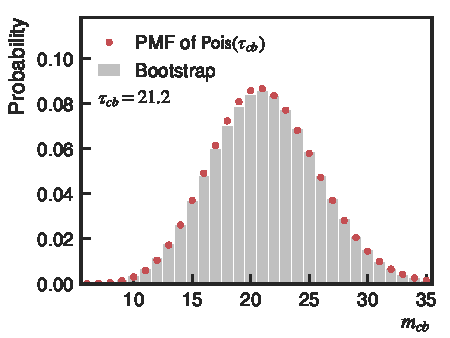
\includegraphics[width=0.98\textwidth]{global_significance/gamma_globs/gamma_obs_251}
    \subcaption{Most signal-like bin of the $\mX = \SI{251}{\GeV}$
      discriminant in the \hadhad-channel.}%
    \label{fig:comparison_bootstrap_poisson_lowest_tau}
  \end{subfigure}\hfill%
  \begin{subfigure}{0.485\textwidth}
    \centering

    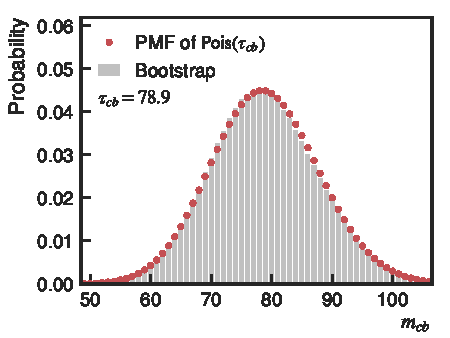
\includegraphics[width=0.98\textwidth]{global_significance/gamma_globs/gamma_obs_1000}
    \subcaption{Most signal-like bin of the $\mX = \SI{1000}{\GeV}$
      discriminant in the \hadhad-channel.}
  \end{subfigure}

  \caption{Comparison of marginal distributions of global observables from the
    Barlow-Beeston method. The red markers show the Poisson distribution used to
    define the constraints on the $\gamma_{cb}$ nuisance parameters
    ($\gamma_{cb} = 1$ is assumed) in the likelihood function. The grey
    histogram shows the distribution of the global observable following the
    Bootstrap approach that accounts for correlations of $m_{cb}$ between
    bins. Statistical uncertainties on the Bootstrap histogram are negligible.}
  \label{fig:comparison_bootstrap_poisson}
\end{figure}


\subsubsection{Global Significance Determination}

In the following the determination of the global significance is discussed using
toy experiments drawn from the background-only model introduced in the previous
sections. The likelihood functions used to perform the discovery tests are
structurally identical to the ones used to obtain the primary results (cf.\
\Cref{sec:statistical_analysis}) only replacing the values of observables and
global observables with the ones drawn from the model.

Before proceeding with the estimation of the global significance, the validity
of the asymptotic approximation used to determine the local significances from
the observed values of the $q_0$ test statistic (i.e.\
$z_{\text{local}} = \sqrt{q_0}$) is examined. For this purpose separate sets of
toy experiments are generated using standard toy generation methods. Standard
methods can be used because the modelling of dependencies between tests is not
required when determining the sampling distribution of the test statistic at the
level of an individual hypothesis test. The quality of the approximation is
investigated, separately for all 20 hypothesis tests, using \num{100000} toy
experiments per test such that the region close to the threshold of interest of
$q_0 \approx 9$ ($z_{\text{local}} \approx 3$) is well populated. A
representative example for the test of the $\mX = \SI{1000}{\GeV}$ signal
hypothesis is shown in~\Cref{fig:q0_samplingdist}. The figure depicts a
comparison of the $q_0$ sampling distributions under the background-only
hypothesis and the resulting relationship between the observed value of $q_0$
and the local significance.

\begin{figure}[htbp]
  \centering

  \begin{subfigure}{0.485\textwidth}
    \centering

    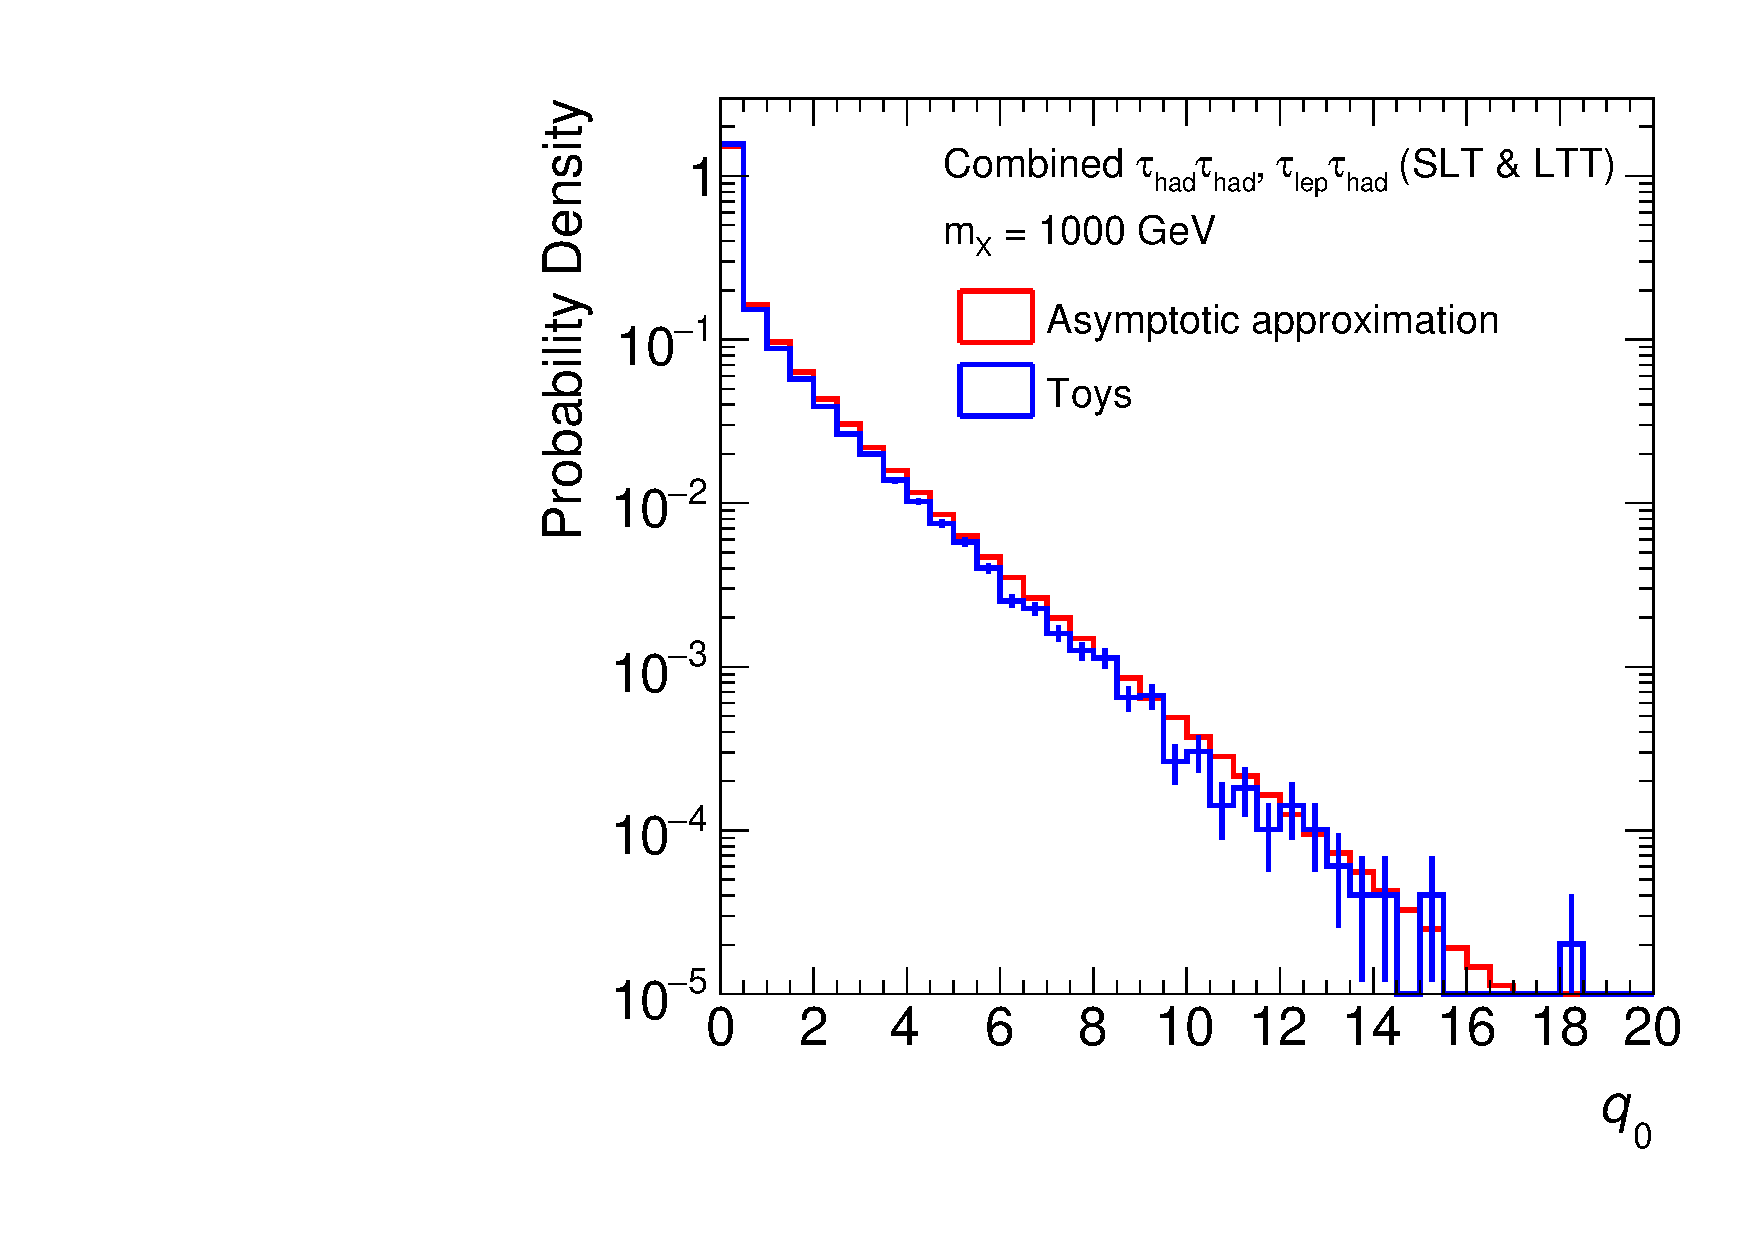
\includegraphics[width=0.98\textwidth]{global_significance/local_sig_toys/q0_1000}
    \subcaption{}
  \end{subfigure}\hfill%
  \begin{subfigure}{0.485\textwidth}
    \centering
    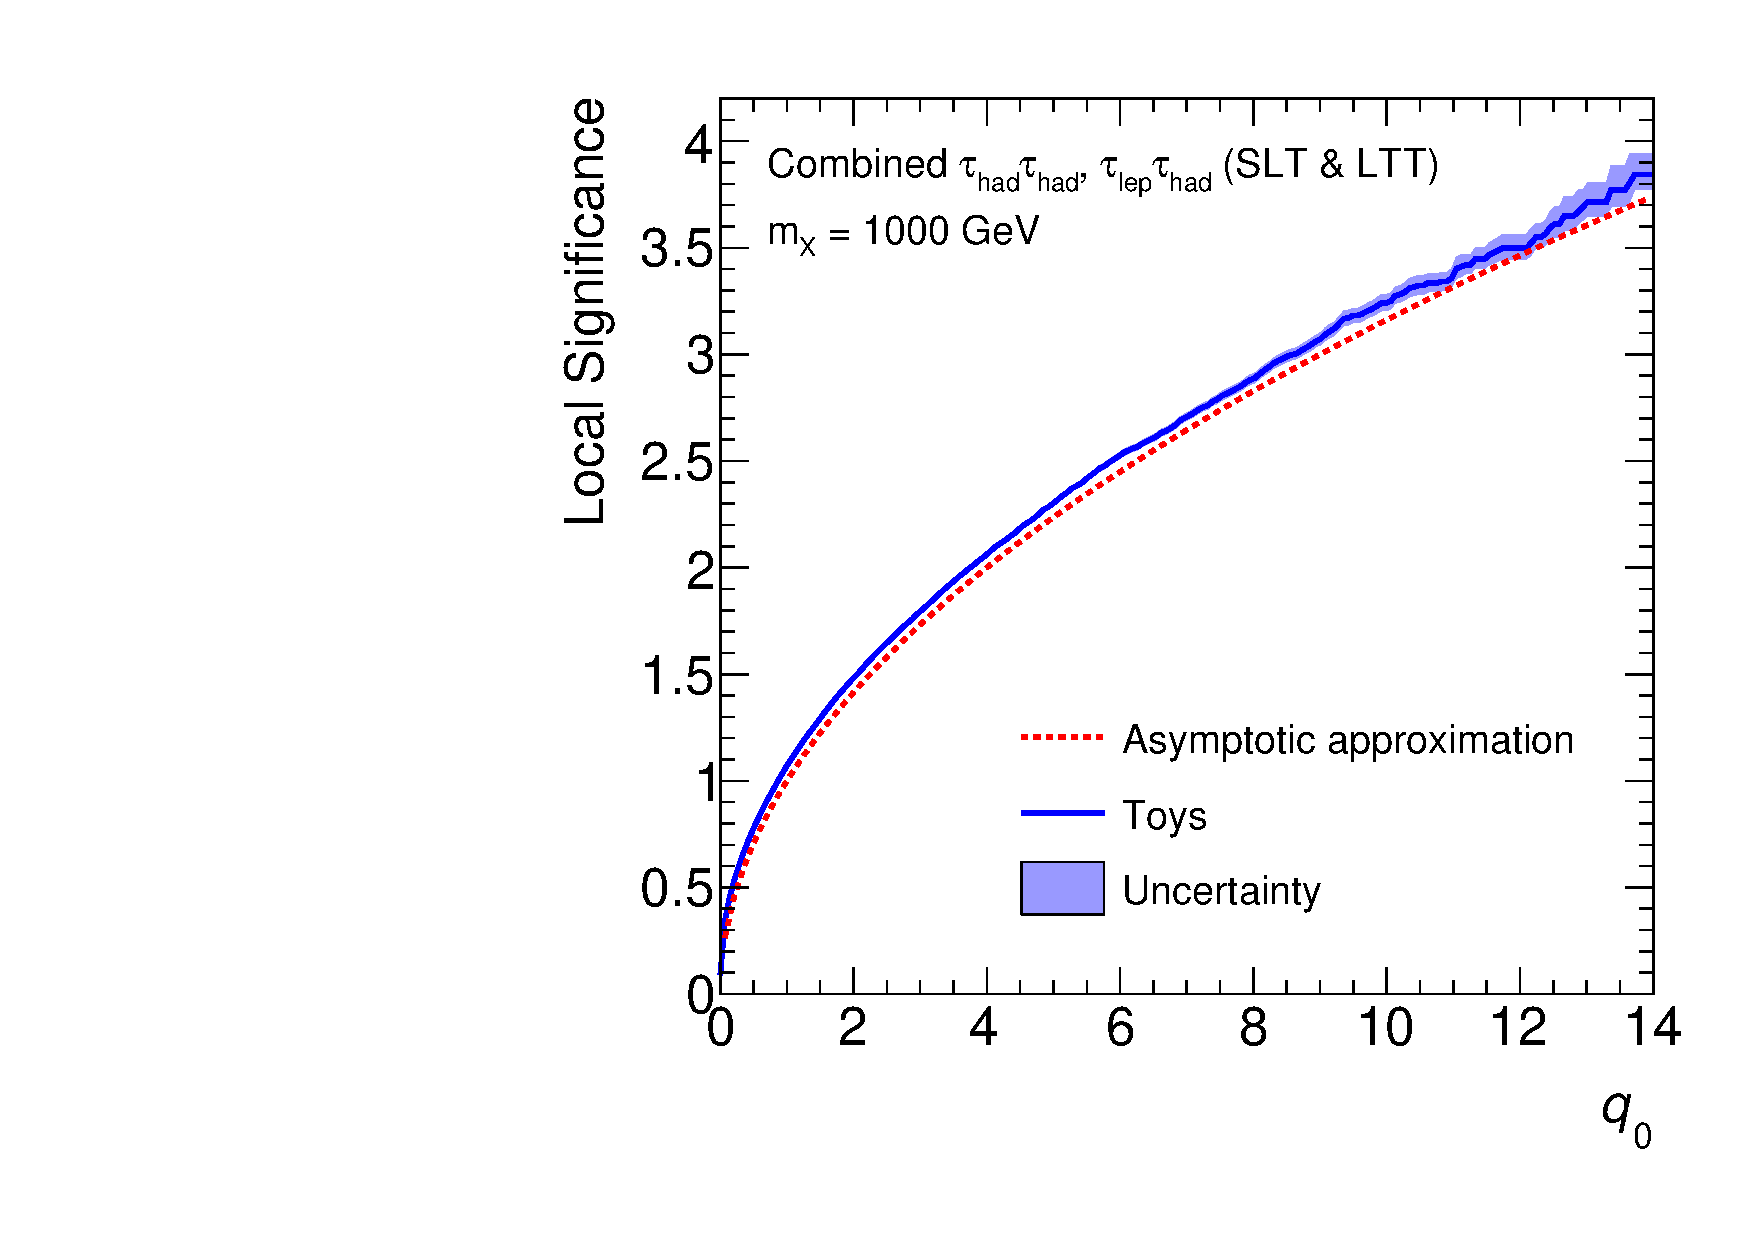
\includegraphics[width=0.98\textwidth]{global_significance/local_sig_toys/q0sig_1000}
    \subcaption{}%
    \label{fig:q0_samplingdist_q0sig}
  \end{subfigure}

  \caption{Comparison of the $q_0$ sampling distribution under the
    background-only hypothesis (a) for the asymptotic approximation and a
    toy-based estimate ($N_{\text{toys}} = \num{100000}$). The resulting
    relationship between the local significance and the observed value of $q_0$
    is depicted in (b). Both are shown for the test of the
    $\mX = \SI{1000}{\GeV}$ hypothesis combining all analysis channels.}%
  \label{fig:q0_samplingdist}
\end{figure}

The asymptotic approximation describes the relationship between the observed
$q_0$ and $z_{\text{local}}$ well for all 20 tests considered in this
analysis. It tends to underestimate the local significance slightly for most
tests, however. For example, the excess observed in data for the test of the
$\mX = \SI{1000}{\GeV}$ hypothesis yields a value of $q_0 = \num{9.08}$
(combination of all analysis channels) resulting in the previously quoted local
significance of \num{3.01} under the asymptotic approximation. The toy-based
estimate yields a local significance of \num{3.09 +- 0.03} which results from
the observed $q_0$ and the result depicted
in~\Cref{fig:q0_samplingdist_q0sig}. The following analysis of the global
significance proceeds using toy-based estimates of local
significances.\footnote{For the purpose of determining the global significance,
  the differences between the asymptotic approximation and the toy-based
  estimate of the $q_0$ sampling distributions have negligible effect on the
  result and lead to the same conclusions.}

A total of \num{10000} toy experiments are performed to ensure that the global
significance can be estimated with a statistical uncertainty below
\num{0.1}. This choice is based on the expectation of the global significance
being close to $2\,\sigma$, which is obtained from analytical calculations under
the assumption that the 20 tests are mutually independent.
% The estimation of the global significance proceeds using the toy
% generation procedure outlined in the previous sections to account for
% dependencies between hypothesis tests.

The following steps performed separately for every toy experiment:
\begin{enumerate}

\item The values of the $q_0$ test statistic are determined for all 20
  hypothesis tests considered in the analysis. This step involves performing a
  conditional ($\sigma = 0$) and an unconditional maximum likelihood fit of the
  model parameters after replacing observables and global observables in the
  likelihood functions with values from the toy experiment.

\item The observed values of $q_0$ are translated to local significances using
  the relationships between $z_{\text{local}}$ and $q_0$.

\item The maximum local significance over all 20 tests is determined.

\end{enumerate}
Performing these steps for all toy experiments yields an estimate of the
distribution of the maximum local significance (over the 20 tests) under the
background-only hypothesis.

The maximum likelihood fits required to obtain the test statistic do not always
succeed. A total of \num{74} fits\footnote{Out of \num{400000} fits, i.e.\
  $20\,\text{(number of tests)} \times 2\,\text{(conditional \& unconditional
    fit)} \times \num{10000}\,\text{(number of toys)}$.}  did not converge even
after retrying the fits with altered optimiser settings. These failures do not
occur randomly but systematically, being restricted to failures of unconditional
fits for cases where a large deficit is observed in the toy data of a bin with
large signal sensitivity. Since a deficit does not constitute a discovery in
this search, the value of $q_0$ is set to 0 in these cases and the toy
experiment is kept.

The result of the toy experiments is shown in~\Cref{fig:zmax_toys} illustrating
the effect of multiple testing leading to an expectation of \Zmaxlocal of about
\num{1.8} even in the absence of a signal. Considering this effect, the global
$p$-value is calculated as the fraction of toy experiments exceeding the
observed~$z_{\text{local}}^{\text{max}}$ in data yielding
\begin{align*}
  \pglobal = \num{0.0222}\numerrt{0.0015}{toy stat.}
\end{align*}
and an equivalent global significance of
\begin{align*}
  z_{\text{global}} = \num{2.01}\numerrt{0.03}{toy stat.} \,\text{,}
\end{align*}
where only statistical uncertainties from the finite number of toy experiments
for the global significance determination are considered.

\begin{figure}[htbp]
  \centering

  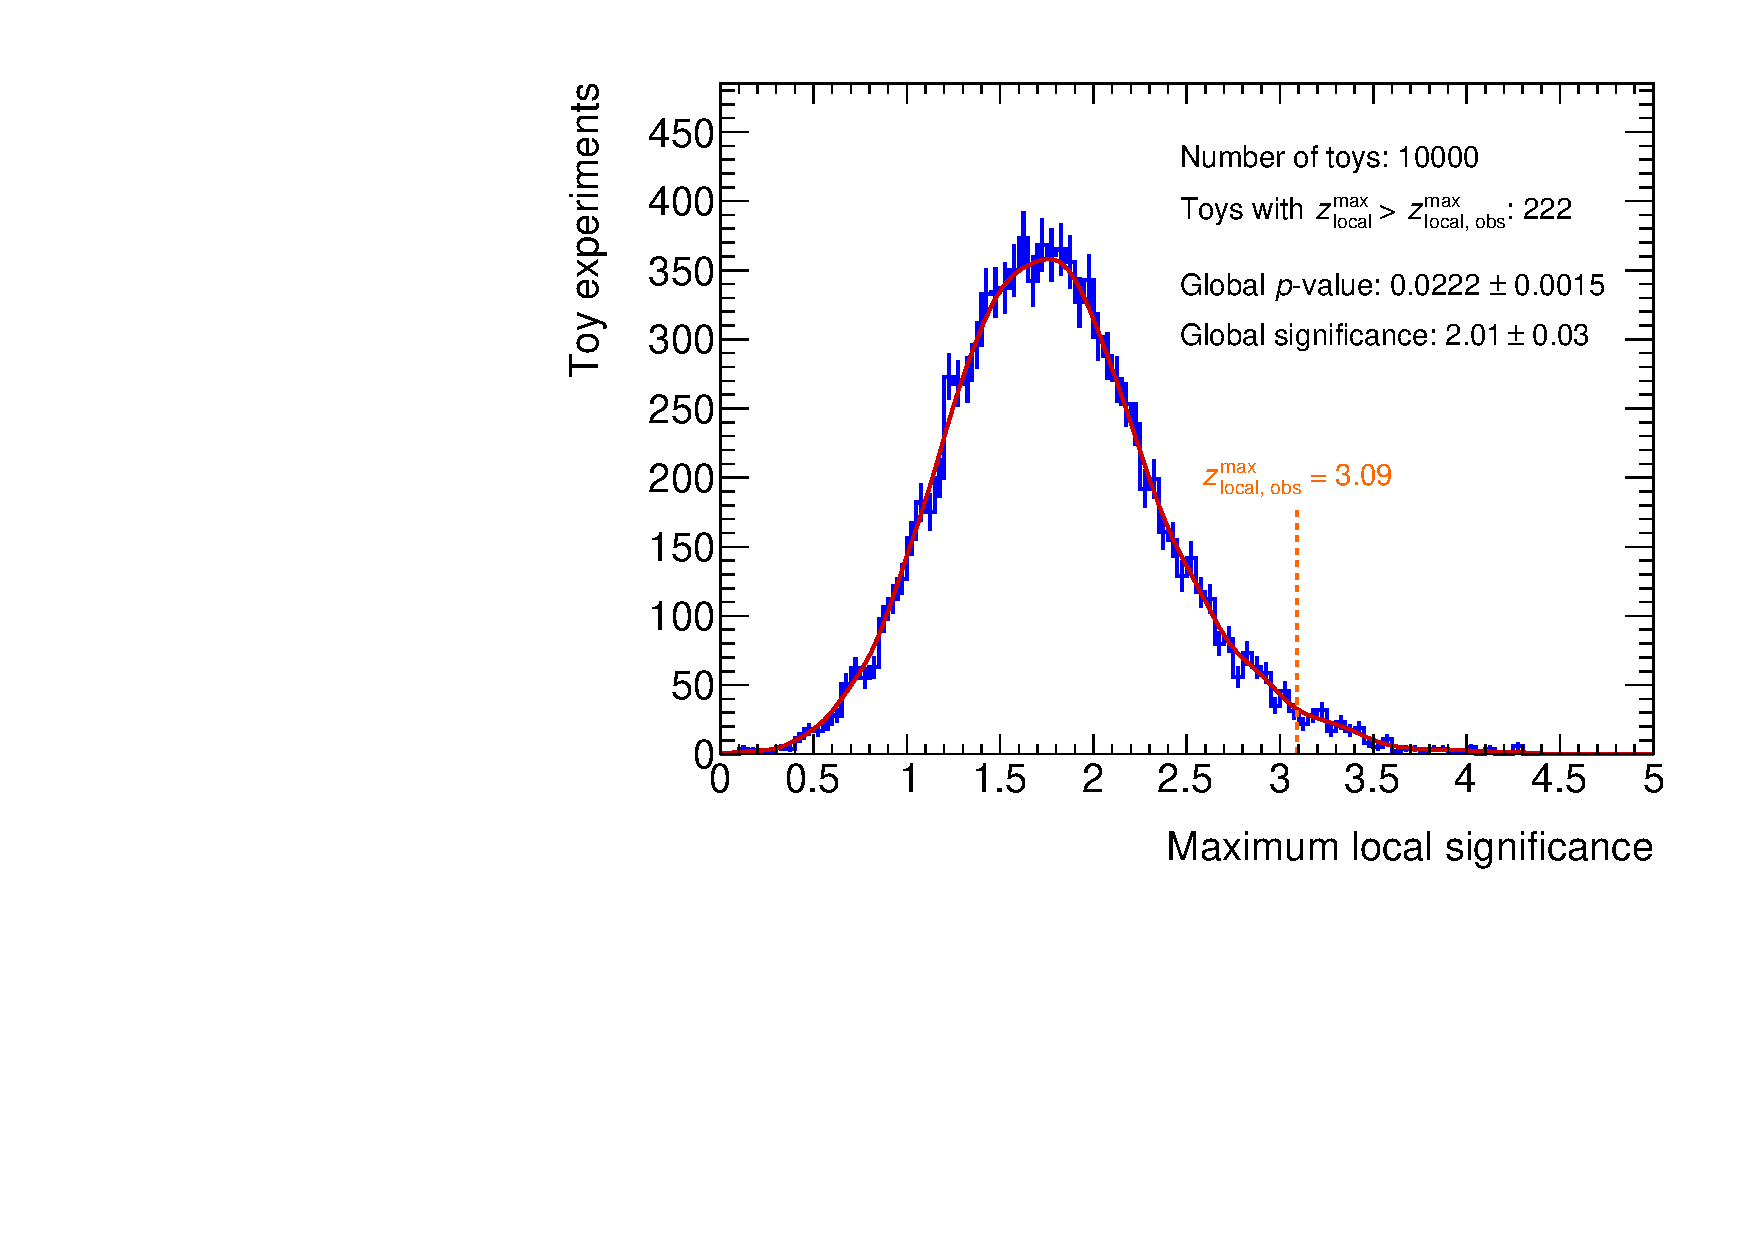
\includegraphics[width=0.62\textwidth]{global_significance/zmax_toys}

  \caption{Estimate of the distribution of the maximum local significance over
    the 20 hypothesis tests considered under the background-only hypothesis
    using toy experiments. The local significance of the excess observed in data
    is indicated in orange. The estimate after kernel smoothing is overlayed in
    red (for illustration only). The quoted uncertainties are from the finite
    number of toy experiments only.}%
  \label{fig:zmax_toys}
\end{figure}

The uncertainty on $z_{\text{global}}$ from the finite number of toy experiments
used to determine the relationships between $q_0$ and $z_{\text{local}}$ is
estimated using the Bootstrap method. The resulting uncertainty on
$z_{\text{global}}$ is \num{0.04} yielding the final result of
\begin{align*}
  z_{\text{global}} = \num{2.01}\numerrt{0.05}{total} \,\text{.}
\end{align*}
% Uncertainties based on modelling assumptions are not included.

\todo[inline]{State that the toy experiments were compared to the
  'standard method' yielding compatible results?}

Furthermore, the toy experiments can be used to estimate the joint distribution
of test statistics for all hypothesis tests under the background-only assumption
to illustrate the dependencies between tests directly. For this purpose, the
signed definition of the discovery significance given
by~$z_{\text{local}}^{\text{signed}} = \sgn(\hat{\sigma}) \sqrt{q_0}$ is used,
with $\sgn(\hat{\sigma})$ being the sign of the best-fit cross-section and
assuming the asymptotic approximation. This choice is made because signed
significances have Standard Normal marginal distributions under the
background-only hypothesis, lending itself for easier interpretation.

\Cref{fig:corr_sig} shows the matrix of linear correlation coefficients between
the signed discovery significances for all 20 tests determined using toy
experiments. It illustrates the linear dependencies between test statistics,
particularly highlighting the increasing dependency between tests for large \mX.

\begin{figure}[htbp]
  \centering

  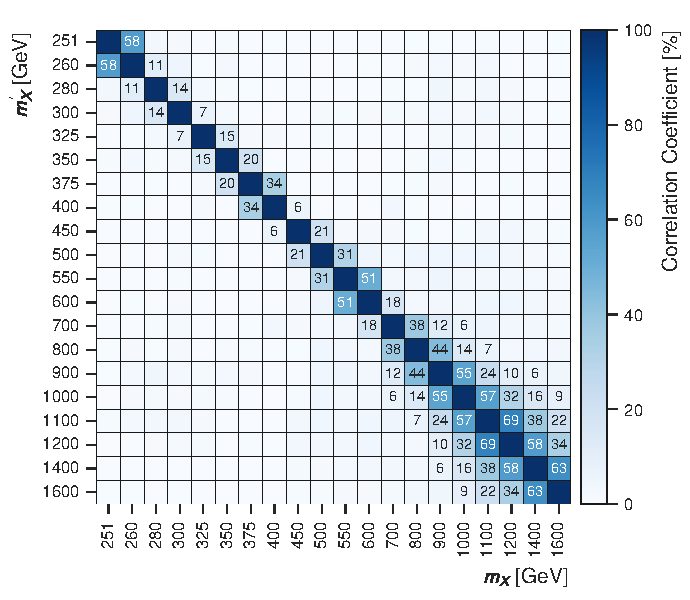
\includegraphics[width=0.7\textwidth]{global_significance/sig_corr}

  \caption{Linear correlation coefficient between signed local significances of
    the 20 hypothesis tests performed for the scalar resonance search under the
    background-only hypothesis. The coefficients are estimated using \num{10000}
    toy experiments drawn from the background-only substitute model. Cells are
    annotated, omitting the diagonal, if the correlation coefficient is greater
    than or equal to \SI{5}{\percent}.}%
  \label{fig:corr_sig}
\end{figure}

Finally, the result of the toy-based estimation of the global significance
yielding $z_{\text{global}} = \num{2.01 +- 0.05}$ is compared to case assuming
that the hypothesis tests can be seen as mutually independent. With this
simplification the global significance is analytically estimated to be \num{2.06
  +- 0.04}, using the observed maximum local significance of \num{3.09 +- 0.03},
which is compatible with the result based on toy experiments. This result might
seem surprising given the large correlation between tests at high \mX shown
in~\Cref{fig:corr_sig}, however, this finding is supported by
simulation. Assuming the joint distribution of signed local significances is
multivariate Normal with zero mean and covariance matrix given
by~\Cref{fig:corr_sig}, the global significance can be estimated from simulation
with negligible statistical precision and compared to the result assuming
independence. The difference in global significance estimates between both
methods amounts to \num{0.02}, concluding that the precision of the toy-based
estimate is not sufficient to differentiate between the cases assuming
independence and linear dependence according to~\Cref{fig:corr_sig}. For
practical purposes, the dependencies between tests performed as part of this
search are weak enough such that the assumption of independence yields
acceptable estimates for the global significance.

In conclusion, the global significance of the excess observed in data for the
test of the $\mX = \SI{1000}{\GeV}$ hypothesis (with a local significance of
$3.1\,\sigma$) is determined to be $2.0\,\sigma$ using a toy-based estimation
method. Uncertainties on the estimated significances are below \num{0.1} and
thus omitted in subsequent discussions for brevity.\todo{Methodological
  uncertainties?}


%%% Local Variables:
%%% mode: latex
%%% TeX-master: "../../phd_thesis"
%%% End:
